\documentclass[a4paper]{report}
\usepackage[utf8]{inputenc}
\usepackage{amsfonts}
\usepackage{amsmath}
\usepackage{amssymb}
\usepackage{euscript}
\usepackage{eufrak}

\newcommand*{\hm}[1]{#1\nobreak\discretionary{}%
            {\hbox{$\mathsurround=0pt #1$}}{}}


\usepackage[english,russian]{babel}
\author{Бахвалов А.Н.}
\title{Лекции по функциональному анализу}

\usepackage{wrapfig}
\usepackage{graphics}

\graphicspath{{images/}}
\ifx\pdfoutput\undefined
\usepackage[dvips]{graphicx}
\else
\usepackage[pdftex]{graphicx}
\usepackage{epstopdf}
\fi
    
    
\begin{document}
\maketitle
\chapter{Метрические пространства}

\noindent\textbf{Определение:} Метрическое пространством называется пара $(M,\rho)$, где $M$ - множество, $\rho:$ 
$M\times M\to[0,+\infty)$ - метрика, удовлетворяющая аксиомам:

1) $\rho(x,y)=0$ $\Leftrightarrow$ $x=y$

2) $\rho(x,y)=\rho(y,x)$

3) $\rho(x,y)\le\rho(x,z)+\rho(z,y)$
\bigskip

\noindent\textbf{Определение:} Последовательность ${x_n}$ называется сходящейся к элементу $x$, если $\rho(x_n,x)\to0$.
Последовательность ${x_n}$ точек $M$ называется фундаментальной в $M$, если $\forall\varepsilon>0$ $\exists N:$ $\forall
m,n>N$ $\rho(x_n,x_m)<\varepsilon$

(Всякая сходящаяся последовательность фундаментальная)
\bigskip

\noindent\textbf{Определение:} Метрическое пространство $(M,\rho)$  называется полным, если в нем каждая фундаментальная
последовательность сходится
\bigskip

\noindent\textbf{Определение:} Нормированным пространством называется пара $(E,\|\cdot\|)$, где $E$ - 
линейное пространство над $\mathbb R$ или $\mathbb C$, а $\|\cdot\|:$ $E\to[0,+\infty)$ удовлетворяет аксиомам:

1) $\|x\|=0$ $\Leftrightarrow$ $x=0$

2) $\|\alpha x\|=\|\alpha\|\cdot\| x\|$, $x\in E$, $\alpha\in\mathbb C$

3) $\|x+y\|\le\|x\|+\|y\|$
\bigskip

Всякое нормированное пространство является метрическим относительно порожденной метрики $\rho(x,y)=\|x-y\|$

Нормированное пространство, полное относительно порожденной метрики, называется банаховым

В метрическом пространстве вводится топология, порожденная открытыми шарами $B_\varepsilon(x)=\{y|\rho(x,y)<\varepsilon\}$
\bigskip

\noindent Примеры метрических и нормированных пространств:

1) Дискретное пространство

$M$ - любое множество, $\rho=\begin{cases} 0,&x=y\\1,&x\ne y\end{cases}$

2) Конечномерное пространство

$\mathbb R^n,\mathbb C^n$, $n\in\mathbb N$

$\|x\|_2=\sqrt{\sum\limits_{k=1}^n|x_k|^2}$, 
$\|x\|_1=\sum\limits_{k=1}^n|x_k|$, $\|x\|_{\infty}=\max\limits_k|x_k|$

3) Пространства последовательностей

$l_p=\left\{{x_n}_{n=1}^\infty|\sum\limits_{n=1}^\infty|x_n|^p<\infty\right\}$, $\|x\|_p=\left(\sum\limits_{n=1}^\infty|x_n|^p\right)^{1/p}$, $1\le p<\infty$

$c=l_\infty=\left\{\{x_n\}_{n=1}^\infty|\sup\limits_n|x_n|<\infty\right\}$, $\|x\|_\infty=\sup\limits_n|x_n|$

$c_0=\left\{\{x_n\}_{n=1}^\infty|\lim\limits_{n\to\infty}x_n=0\right\}$, $\|x\|_{c_0}=\max\limits_n|x_n|$

$c_{0,0}=\left\{\{x_n\}_{n=1}^\infty|\exists N:\forall n>N\quad x_n=0\right\}$, $\|x\|_{c_{0,0}}=\max\limits_n|x_n|$

4) $C([a,b])$ - пространство непрерывных на $[a,b]$ функций с нормой 

$\|f\|=\max\limits_{x\in[a,b]}|f(x)|$

\noindent
\begin{wrapfigure}[5]{r}{0.4\linewidth} 
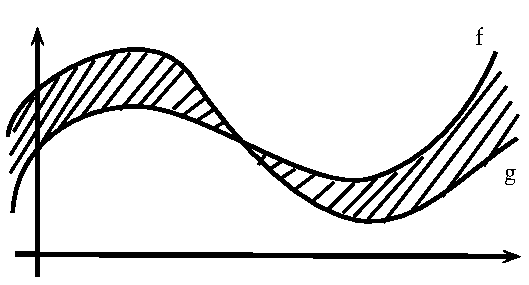
\includegraphics[width=\linewidth]{1}
\end{wrapfigure}

5) $C_1([a,b])$ - множество непрерывных функций с нормой $\|f\|=\displaystyle\int\limits_a^b|f(x)|dx$

В данной метрике $\|f-g\|=\displaystyle\int\limits_a^b|f-g|dx$, что есть площадь фигуры

$C_1([0,1])$ не полно

$\square$ Рассмотрим функцию $f_n=\begin{cases}0,&0\le x\le\frac12\\n(x-\frac12),&\frac12\le x\le\frac12+\frac1n\\1,&\frac12+\frac1n\le x_n\le1\end{cases}$

\begin{wrapfigure}[3]{L}{0.3\linewidth} 
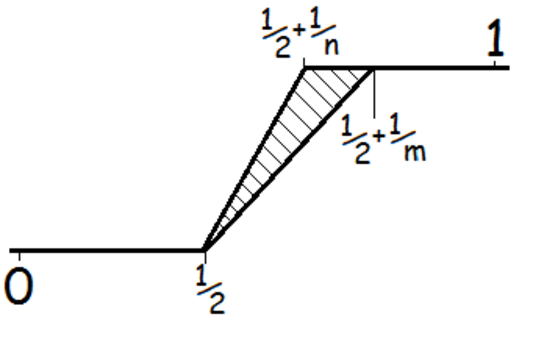
\includegraphics[width=\linewidth]{2}
\end{wrapfigure}

\noindent
$\|f_n-f_m\|=\frac12|\frac1n-\frac1m|\xrightarrow[n,m\to\infty]{}0$ 

\noindent
$\{f_n\}$ фундаментальна, но 

$f_n(x)\to\begin{cases}0,&x\le\frac12\\1,x>\frac12\end{cases}$ - разрывная $\blacksquare$

\bigskip
\bigskip
\bigskip
\noindent\textbf{Определение:} Пусть $(M,\rho)$ - метрическое пространство. Его подпространством называется пара $(M_1,\rho|_{M_1\times M_1})$, 
где $M_1\subset M$ (для простоты пишут просто $(M_1,\rho)$ или $M_1$)
\bigskip

\noindent\textbf{Определение:} Пусть $(E,\|\cdot\|)$ -  нормированное пространство, то его подпространством называется пара 
$(E_1,\|\cdot\|_{E_1})$, где $E_1\subset E$, $E_1$ - линейное подпространство в $E$ 
\bigskip

\noindent\textbf{Определение:} Пусть $(M,\rho)$ и $(N,d)$ - метрические пространства. Отображение $f\colon M\to N$ называется
изометрией, если:

1) $f$ - биективно

2) $\forall x,y\in M\quad d(f(x),f(y))=\rho(x,y)$

Изометрия переводит сходящиеся последовательности в сходящиеся, фундаментальные в фундаментальные $\Rightarrow$ два 
изометричных пространства либо оба полны, либо оба неполны
\bigskip

\noindent\textbf{Определение:} Отображение нормированных пространств называется изометрическим изоморфизмом, если оно 
является изометрией и сохраняет линейную структуру
\bigskip

\noindent\textbf{Определение:} Метрическое пространство $(N,d)$ называется пополнением метрического пространства $(M,\rho)$, если:

1) $(N,d)$ - полно

2) $\exists N_1$ - всюду плотное в $N$ и $\exists$ изометрия $f\colon (M,\rho)\to(N_1,d)$
\bigskip

\noindent\textbf{Примеры:} Любое полное пространство является своим пополнением; $\mathbb R$ - пополнение $\mathbb Q$
\bigskip

\noindent\textbf{Лемма 1.1} Пусть $(M,\rho)$ - полное метрическое пространство $\colon M_1\subset M$. Тогда $(M_1,\rho)$ 
полно тогда и только тогда, когда $M_1$ - замкнуто, и если $M_1$ не замкнуто, то $(\bar M_1,\rho)$ будет его пополнением

\noindent $\square$ $\Rightarrow)$ Пусть $(M_1,\rho)$ - полное, $x_n\in M_1$, $x\in M$, $\rho(x_n,x)\to0$

Тогда $\{x_n\}$ фундаментальна в $M$ $\Rightarrow$ в $M_1$ $\Rightarrow$ в силу полноты

 $\exists y\in M_1\colon\rho(x_n,y)\to0$
$\Rightarrow$ $x=y$ $\Rightarrow$ $x\in M_1$ $\Rightarrow$ $M_1$ замкнуто

$\Leftarrow)$ Пусть $M_1$ - замкнуто. Предположим, что оно не полно, т.е. $\exists\{x_n\}$ - фундаментальная в $M_1$, 
но не сходящаяся, тогда $\{x_n\}$ - фундаментальная в $M$ $\Rightarrow$ $\exists x\in M\colon x_n\to x\in M\setminus M_1$
$\Rightarrow$ $M_1$ не замкнуто

(+) Пусть $M_1$ не замкнуто. $\bar M_1$ - замкнуто, $M_1$ всюду плотно в $M_1$. По доказанному, $(\bar M_1,\rho)$ - 
полно. Все условия определения пополнения выполнены для $d=\rho$, $f(x)=x$, $N=\bar M_1$ $\blacksquare$
\bigskip

\noindent\textbf{Лемма 1.2:} Если $\{x_n\}$ - фундаментальная в метрическом пространстве $M$, $\exists\{n_k\}\colon
x_{n_k}\to x\in M$, то $x_n\to x$

\noindent $\square$ $\rho(x_n,x)\le\rho(x_{n_k},x)+\rho(x_n,x_{n_k})$ $\blacksquare$
\bigskip

\noindent\textbf{Определение:} Замкнутым шаром в метрическом пространстве называется $\bar B_\varepsilon(x)=\{y\in M\colon
\rho(x,y)\le\varepsilon\}$
\bigskip

\noindent\textbf{Теорема 1.1:} (Принцип вложенных шаров) Метрическое пространство $(M,\rho)$ полно т. и т. т., к. $\forall$
последовательности шаров $\bar B_n=\bar B_{r_n}(x_n)$, такой, что $\bar B_n\supset\bar B_{n+1}$, и $r_n\to0$, $\exists$ 
общая точка $x\in\bigcap\limits_{n=1}^\infty\bar B_n$

\noindent $\square$ $\Rightarrow$) Пусть пространство полно. По неравенству треугольника $\forall n,m\colon n<m\quad
\rho(x_n,x_m)\le r_n$ $\Rightarrow$ $\{x_n\}$ - фундаментальная последовательность, т. к. $r_n\to0$ $\Rightarrow$ 
$\exists x=\lim\limits_{n\to\infty} x_n$

$\forall n$ $B_n$ - замкнут, $\forall m>N\quad x_m\in B_n$ $\Rightarrow$ $x\in\bar B_n$ $\Rightarrow$ $x\subset\bigcap\limits_n
\bar B_n$

$\Leftarrow$) Пусть выполнено условие на шары, $\{x_n\}$ - фундаментальная

$\forall k\quad\exists n_k\colon n,m\ge n_k\rho(x_n,x_m)\le\displaystyle\frac{1}{2^k}$, $\{n_k\}$ - возрастающая

Рассмотрим шары $\bar B_k=\bar B_{\displaystyle\frac{2}{2^k}}(x_{n_k})$

$\forall x\in\bar B_{k+1}\quad \rho(x,x_{n_k})\le\rho(x,x_{n_{k+1}})+\rho(x_{n_{k+1}},x_{n_k})\le\displaystyle\frac{2}{2^{k+1}}+\displaystyle\frac{1}{2^k}=
\displaystyle\frac{2}{2^k}$ $\Rightarrow$ $\bar b_{k+1}\subset\bar B_k$ $\Rightarrow$ $\exists x\in\bigcap\limits_{k=1}^\infty\bar B_k$; 
тогда $\forall k\quad\rho(x,x_{n_k})\le\displaystyle\frac{2}{2^k}$ $\Rightarrow$ $x_{n_k}\to x$ 

$\Rightarrow$ по лемме 1.2 $x_n\to x$ $\blacksquare$
\bigskip

\noindent\textbf{Определение:} Множество $A$ в метрическом пространстве $M$ называется нигде не плотным в $M$, если $\forall$
шара $B$ в $M$ $\exists$ шар $\bar B_1\subset B\colon\bar B_1\cap A=\varnothing$
\bigskip

\noindent\textbf{Теорема 1.2:} (Бэр) Пусть $(M,\rho)$ - полное метрическое пространство, $A_n$ - нигде не плотное в $M$. 
Тогда $C=M\setminus\bigcup\limits_{n=1}^\infty A_n$ всюду плотно в $M$

\noindent $\square$ Пусть $B$ - шар в $M$. Т. к. $A_1$ нигде не плотно, то $\exists$ шар $\bar B_1\subset B$ c радиусом 
$r_1<\frac12\colon\bar B_1\cap A=\varnothing$

Если построены $\bar B_1\supset\bar B_2\supset\ldots\supset\bar B_{n-1}$, то в силу нигде не плотности $A_n$ $\exists$ 
шар $\bar B_n\subset\bar B_{n-1}$ с радиусом $r_n<\frac1n\colon\bar B_n\cap A_n=\varnothing$

По теореме 1.1 $\exists x\in\bigcap\limits_{n=1}^\infty\bar B_n$. Тогда $x\in B$, $\forall x\notin A_n$ $\Rightarrow$ 
$x\in C\cap B$ $\Rightarrow$ 

$C$ всюду плотно $\blacksquare$
\bigskip

\noindent\textbf{Следствие:} Полное метрическое пространство не может быть представлено как не более чем счетное объединение 
нигде не плотных множеств
\bigskip

\noindent\textbf{Теорема 1.3:} (Принцип сжимающихся отображений) Пусть $M$ - полное множество, $f\colon M\to M$, 
$\exists q\in(0,1)$ $\forall x,y\in M$ $\rho\left(f(x),f(y)\right)\le q\rho(x,y)$ (сжимающееся отображение), тогда 
$\exists!\quad x\in M\colon f(x)=x$

\noindent $\square$ Возьмем произвольно $x_1\in M$ и по индукции положим $x_{k+1}=f(x_k)$. Покажем, что $\{x_k\}$ - 
фундаментальная

Пусть $n<m$ $\Rightarrow$ по неравенству треугольника $\rho(x_n,x_m)\le\sum\limits_{k=n}^{m-1}\rho(x_k,x_{k+1})$, 
где $\rho(x_k,x_{k+1})\le q\rho(x_{k-1},x_k)\le\ldots\le q^{n-1}\rho(x_1,x_2)$, поэтому $\rho(x_n,x_m)\le\rho(x_1,x_2)
\sum\limits_{k=n}^{m-1}q^{k-1}\le\rho(x_1,x_2)\displaystyle\frac{q^{n-1}}{1-q}\xrightarrow[n\to\infty]{}0$

$\Rightarrow$ $\{x_n\}$ - фундаментальная $\Rightarrow$ $\exists x\colon x_n\to x$

Заметим, что $f$ - непрерывно на $M$. Переходим к пределу в равенстве $x_{k+1}=f(x_k)$, получим $x=f(x)$. 

\noindent Если к тому же 
$y=f(y)$, то $\rho(f(x),f(y))\le q\rho(x,y)$ $\Rightarrow$ $\rho(x,y)=0$, $y=x$ $\blacksquare$
\bigskip

\noindent\textbf{Лемма 1.3:} Пусть $x_n\to x$, $y_n\to y$, тогда $\rho(x_n,y_n)\to\rho(x,y)$

\noindent $\square$ $\rho(x_n,y_n)\le\rho(x_n,x)+\rho(x,y)+\rho(y,y_n)$

$\rho(x,y)\le\rho(x,x_n)+\rho(x_n,y_n)+\rho(y_n,y)$

$|\rho(x,y)-\rho(x_n,y_n)|\le\rho(x_n,x)+\rho(y_n,y)$ $\blacksquare$
\bigskip

\noindent\textbf{Лемма 1.4:} Пусть $(M,\rho)$ и $(N,d)$ - полные метрические пространства, $M_1,N_1$ - всюду плотные 
подмножества в $M,N$ соответственно, $f$ - изометрия $\colon M_1\to N_1$ тогда она единственным образом продолжается до 
изометрии $M\to N$

\noindent $\square$ Пусть $x_n\in M_1\to x\in M$

$\{x_n\}$ - фундаментальная $\Rightarrow$ $\{f(x_n)\}$ также фундаментальная, т. к. $f$ - изометрия $\Rightarrow$ т. к. 
$N$ полно, то $\exists y\in N\colon f(x_n)\to y$. Тогда $f(x)=y$ - единственно возможное отображение

Если $x_n'\to x$, $f(x_n')\to y'\ne y$, то $\{\tilde x_n\}=\{x_1,x_1',x_2,x_2',\ldots\}$ сходится к $x$ $\Rightarrow$ 
$\exists\lim f\{\tilde x_n\}$ $\Rightarrow$ $y'=y$ и $f$ доопределено корректно

Если $x',x''\to M$, $M_1\ni x_n'\to x'$, $M_1\ni x_n''\to x''$, то 

$\rho(x_n',x_n'')\xrightarrow[]{\text{л. 1.3}}\rho(x',x'')$

$\rho(x_n',x_n'')=d(f(x_n'),f(x_n''))\xrightarrow[]{\text{л. 1.3}}d(f(x'),f(x''))$, т. е. продолженное $f$ сохраняет расстояние

Пусть $y\in N$, тогда $\exists y_n\in N_1\colon y_n\to y$, т. к. $f$ - изометрия $M_1$ и $N_1$, то $\exists x_n\in M_1$ 
$f(x_n)=y_n$, $\{y_n\}$ - фундаментальная в $N$ $\Rightarrow$ $\{x_n\}$ фундаментальная в $M$ $\Rightarrow$ в силу 
полноты $M$ $\exists x\in M\colon x_n\to x$. 

По построению $f(x)=y$, т. е. образ продолженного $f$ есть все $N$ $\blacksquare$
\bigskip

\noindent\textbf{Теорема 1.4:} (1) Для всякого метрического пространства существует пополнение

(2) Любые два пополнения одного метрического пространства изометричны

\noindent $\square$ (2) Пусть $(N',d')$ и $(N'',d'')$ - два пополнения, $f'\colon M\to N_1'$ и $f''\colon M\to N_1''$ - изометрии

$\Rightarrow$ $f''\circ(f')^{-1}$ - изометрия $N_1'\to N_1''$

По лемме 1.4 это отображение продолжается до изометрии $N'\to N''$

(1) Пусть $\{x_n\}$ и $\{y_n\}$ - две фундаментальные последовательности в $M$. Тогда $\exists\lim\limits_{n\to\infty}\rho(x_n,y_n)$

$|\rho(x_n,y_n)-\rho(x_m,y_m)|\le\rho(x_n,y_m)+\rho(y_n,y_m)$

$\{\rho(y_n,y_m)\}$  - фундаментальная $\Rightarrow$ $\exists\lim\rho(x_n,y_n)$

На множестве всех фундаментальных последовательностей элементов $M$ введем отношение эквивалентности $\{x_n\}\sim\{y_n\}$, 
если $\lim\limits_{n\to\infty}\rho(x_n,y_n)=0$

Пусть $N=\left\{\{x_n\}\right\}|_\infty$ - множество классов эквивалентности

$d(\{x_n\},\{y_n\})=\lim\limits_{n\to\infty}\rho(x_n,y_n)$

Заметим, что т. к. $\rho(x_n,y_n)\le\rho(x_n,z_n)+\rho(z_n,y_n)$, то в пределе 

$d(\{x_n\},\{y_n\})\le d(\{x_n\},\{y_n\})+\rho(\{z_n\},\{y_n\})$

$\Rightarrow$ (а) отношение $"\sim"$ транзитивно; (б) в $N$ выполнено неравенство треугольника

Заметим, что множество $N_1$ стационарных последовательностей (их классов эквивалентности) изометрично $M\colon
x_0\stackrel{f}{\longmapsto}\{x_n\}$, $x_n\equiv x_0$

Если $x=\{x_n\}$ - фундаментальная в $M$, $x^n\colon x_k^n=x_n$, то $d(x,x^n)\hm=\lim\limits_{k\to\infty}\rho(x_k,x_n)\le
\sup\limits_{k>n}\rho(x_k,x_n)\xrightarrow[n\to\infty]{}0$ $\Rightarrow$ $d(x,x^n)\to0$ 

$\Rightarrow$ $N_1$ всюду плотно в $N$

Проверим полноту $(N,d)$. Пусть $x^n=\{x_k^n\}_{k=1}^\infty$, где $\{x^n\}$ - фундаментальная последовательность в $N$. 
Т. к. $\{x_n^k\}_{k=1}^\infty$ - фундаментальная, то

 $\exists m_n\colon\forall k,l\ge m_n\quad\rho(x_k^n,x_l^n)<\displaystyle\frac{1}{2^n}$
и можно считать, что $m_n>m_{n-1}$

Пусть $x=\{x_{m_k}^k\}$. Покажем, что $x\in N$ и что $d(x^n,x)\to0$

Для достаточно большого n $(n>m_k,n>m_l)$ имеем: 

$\rho(x_{m_k}^k,x_{m_l}^l)\le\rho(x_{m_k}^k,x_n^k)+\rho(x_n^k,x_n^l)+\rho(x_n^l,x_{m_l}^l)\displaystyle\le\frac{1}{2^k}+\left(d(x^k,x^l)+
\displaystyle\frac{1}{2^k}+\frac{1}{2^l}\right)\hm+\displaystyle\frac{1}{2^l}\xrightarrow[k,l\to\infty]{}0$, т. е. $x$ - фундаментальная

Наконец, $d(x^n,x)=\lim\limits_{k\to\infty}(x_k^n,x_{m_k}^k)$, где $\rho(x_k^n,x_{m_k}^k)\le\rho(x_{m_k}^n,x_{m_k}^k)+
\rho(x_k^n,x_{m_k}^n)\le$

\noindent$\le d(x^n,x^k)+o(1)_{m_k\to\infty}+\displaystyle\frac{1}{2^n}<\varepsilon$ при достаточно большом $n$.

Итак, $(N,d)$ полно $\blacksquare$
\bigskip

\noindent\textbf{Замечание:} Любое нормированное пространство можно пополнить как метрическое
\bigskip

\noindent\textbf{Определение:} Пополнением нормированного пространства $(E,\|\cdot\|_E)$ называется банахово пространство 
$(F,\|\cdot\|_F)\colon\exists$ изометрический изоморфизм $E\to F_1\subset F$, где $F_1$ - линейное подпространство, 
плотное в $F$
\bigskip

Можно проверить, что Т. 1.4 переносится на случай нормированных пространств, если ввести на пространстве фунжаментальных 
последовательностей линейные операции как $\alpha\{x_n\}+\beta\{y_n\}=\{\alpha x_n+\beta y_n\}$








\chapter{Компактность в метрических пространствах}

\noindent\textbf{Определение:} Множество в метрическом пространстве называется компактным, если из любого его покрытия 
открытыми множествами можно выбрать конечное покрытие

Множество называется предкомпактным, если его замыкание компактно
\bigskip

\noindent\textbf{Лемма 2.1:} Компактное множество в метрическом пространстве ограничено (лежит в нектором шаре) и замкнуто

\noindent $\square$ Пусть $K$ - компактное множество. Фиксируем $x\in M$, тогда шары $\{B_n(x)\}_{n\in\mathbb N}$ 
покрывают $K$. Выберем конечное подпокрытие из шаров $B_{n_j}(x)$, $n_1<n_2\hm<\ldots<n_m$ $\Rightarrow$ $K\subset
B_{n_m}(x)$ $\Rightarrow$ ограничено

Пусть $x\notin K$ $\Rightarrow$ $\forall y\in K\quad\exists$ шары $U_y\ni x$ и $V_y\ni y\colon U_y\cap V_y=\varnothing$

$\{V_y\}_{y\in K}$ покрывают $K$; выберем конечное подпокрытие $H\subset\bigcup\limits_{j=1}^n V_{y_j}$ 

$\Rightarrow$
$\bigcap\limits_{j=1}^n U_{y_j}$ - окрестность $x$, не пересекающаяся с $\bigcup\limits_{j=1}^n V_{y_j}$ и тем более с $K$ 

$\Rightarrow$ $x$ - внешняя точка $K$ $\Rightarrow$ $M\setminus K$ открыто, $K$ - замкнуто $\blacksquare$
\bigskip

\noindent\textbf{Определение:} Множество $A$ называется $\varepsilon$-сетью для множества $B$ в метрическом пространстве 
$M$ $(\varepsilon>0)$, если $\forall x\in B\quad\exists y\in A\colon\rho(x,y)\le\varepsilon$
\bigskip

\noindent\textbf{Определение:} Множество $A$ в метрическом пространстве $M$ называется вполне ограниченным, если $\forall
\varepsilon>0$ $\exists$ конечная $\varepsilon$-сеть для $A$
\bigskip

\noindent\textbf{Определение:} Метрическое пространство называется сепарабельным, если в нем есть не более чем счетное 
всюду плотное множество. Множество в метрическом пространстве называется сепарабельным, если оно сепарабельно как 
подпространство
\bigskip

\noindent\textbf{Лемма 2.2:} Если множество $B$ в метрическом пространстве $M$ имеет $\varepsilon$-сеть, то можно построить
$2\varepsilon$-сеть для $B$, состоящую из элементов $B$ и имеющую ту же мощность

\noindent $\square$ Пусть $\{x_n\}$ - $\varepsilon$-сеть для $B$. Если для данного $n$ множество $B\cap\bar B_\varepsilon(x_n)$ 
пусто, то выкинем $x_n$ из сети, сеть останется $\varepsilon$-сетью

Для оставшихся зафиксируем $y_n\in B\cap\bar B_\varepsilon(x_n)$. Проверим $\{y_n\}$ - искомая

$\forall x\in B\quad\exists n\colon\rho(x,x_n)\le\varepsilon$ $\Rightarrow$ $\rho(x,y_n)\le\rho(x,x_n)+\rho(x_n,y_n)
\le 2\varepsilon$ $\blacksquare$
\bigskip

\noindent\textbf{Лемма 2.3:} Пусть $\varepsilon>0$, $\alpha>1$, $B$ есть $\varepsilon$-сеть для $A$. Тогда $B$ есть 
$\alpha\varepsilon$-сеть для $\bar A$

\noindent $\square$ $\forall x\in\bar A\quad\exists y\in A\colon\rho(x,y)<(\alpha-1)\varepsilon$;
$\exists z\in B\colon\rho(y,z)\le\varepsilon$

 По неравенству треугольника, $\rho(x,z)<\alpha\varepsilon$ $\blacksquare$
\bigskip


\noindent\textbf{Следствие:} Если $A$ вполне ограничено, то $\bar A$ вполне ограничено
\bigskip

\noindent\textbf{Определение:} Пусть $(x,\tau)$ - топологическое пространство. Система множеств $\tau_0<\tau$ называется базой
топологии $\tau$, если 

$\forall U\subset\tau\quad\forall x\in U\quad\exists V\in\tau_0\colon x\in V\subset U$
\bigskip

\noindent\textbf{Пример:} Если $(M,\rho)$ - метрическое пространство, то $\{B_r(x)\}_{x\in M,r>0}$ - база топологии
\bigskip

\noindent\textbf{Лемма 2.4:} Топология сепарабельного метрического пространства имеет счетную базу

\noindent $\square$ Пусть $\{x_n\}$ - счетное всюду плотное в метическом пространстве $(M,\rho)$. Докажем, что система 
$\{B_{\frac1k}(x_n)\}_k$, $n\in\mathbb N$ - база топологии.

Пусть $x\in M$, $U\in\tau$. Тогда $\exists r>0\colon B_r(x)\subset U$

$\exists k\colon\frac2k<r$; $\exists n\colon\rho(x,x_n)<\frac1k$ 

Тогда $x\in B_{\frac1k}(x_n)\subset B_{\frac2k}(x)$

Если $\rho(x_n,y)<\frac1k$, то $\rho(x,y)\le\rho(x,x_n)+\rho(x_n,y)<
\frac1k+\frac1k=\frac2k$

Но $B_{\frac2k}(x)\subset B_r(x)\subset U$, т. е. $x\in B_{\frac1k}(x_n)\subset U$ $\blacksquare$
\bigskip

\noindent\textbf{Лемма 2.5:} Если множество $A$ в метрическом пространстве вполне ограничено, то $A$ сепарабельно

\noindent $\square$ Пусть $\{x_{k,j}\}_{j=1}^{j_k}$ - конечная $\frac1k$-сеть

Тогда $\{x_{kj}\}_{j=1,k=1}^{j_k,\infty}$ - всюду плотно в $A$ $\blacksquare$
\bigskip

\noindent\textbf{Теорема 2.1:} (Линделеф) Пусть $(x,\tau)$ - топологическое пространство cо счетной базой топологии 
$\{V_n\}_{n=1}^\infty$ (в частности, сепарабельная метрика) 

$E\subset X$, $U_\alpha\in\tau$, $E\subset\bigcup\limits_\alpha
U_\alpha$. 

Тогда $\exists$ не более чем счетное подпокрытие $E\subset\bigcup\limits_{n=1}^\infty U_{\alpha_n}$

\noindent $\square$ Если для данного $n$ $\exists\alpha\colon V_n\subset U_\alpha$, то зафиксируем одно такое $\alpha_n$, 
что $V_n\hm\subset U_{\alpha_n}$. Если такого $\alpha$ нет, то не фиксируем его. Покажем, что $\exists x\subset
\bigcup\limits_n U_{\alpha_n}$

 Если $x\in E$, то $\exists\alpha\colon x\in U_\alpha$ $\Rightarrow$ $\exists n\colon x\in
V_n\subset U_\alpha$

$\Rightarrow$ $\alpha_n$ было выбрано, $x\in V_n\subset U_{\alpha_n}$ $\blacksquare$
\bigskip

\noindent\textbf{Лемма 2.6:} Множество $K$ в метрическом пространстве $M$ вполне ограничено т. и т. т., к. из любой 
последовательности его точек можно выбрать фундаментальную подпоследовательность

\noindent $\square$ $\Rightarrow$) Если в последовательности $\{x_n\}$ есть бесконечное число одинаковых членов, то 
утверждение верно. 

Пусть это не так $\Rightarrow$ $\exists$ бесконечное число различных $\{x_n\}$. Рассмотрим $\{y_{n,1}\}$ - конечная 
1-сеть для $K$. Для некоторого $n_1^0\colon$ на расстоянии не более 1 от $y_{n_1^0,1}$ есть бесконечное число точек $x_n$.

Пусть $A_1$ - множество точек $x_n\colon\rho(x_n,y_{n_1^0,1})\le1$. $A_1$ - бесконечно и вполне ограничено (т.к. $A_1
\subset K$, $K$ - вполне ограничено). Пусть $\{y_{n,2}\}$ - конечная $\frac12$-сеть для $A_1$. $\exists\quad n_2^0\colon$ 
множество $A_2=\{x_n\in A_1\colon\rho(y_{n_2^0,2,x_n})\le\frac12\}$ бесконечно

По индукции $\exists$ бесконечное множество $A_j\subset A_{j-1}\colon$ 

$\exists y_{n_j^0,i}\colon\forall x\in A_j\quad
\rho(y_{n_j^0,j},x_i)\le\displaystyle\frac{1}{2^j}$

Тогда $\forall x',x''\in A\quad\rho(x',x'')\le\displaystyle\frac{1}{2^{i-1}}$, взяв по индукции попарно различные $x_{n_j}\in A$, 
получим фундаментальную подпоследовательность

$\Leftarrow$) Пусть $K$ - не вполне ограничено. $\exists\varepsilon>0\colon K$ не имеет конечной $\varepsilon$-сети. 
Возьмем $x_1\in K$ - любое. $\exists x_2\in K\colon\rho(x_2,x_1)>\varepsilon$ (иначе $\{x_1\}$ - $\varepsilon$-сеть). 
Пусть построены $\{x_k\}_{k=1}^n\colon\forall k\ne j\quad\rho(x_k,x_j)>\varepsilon$

Тогда $\exists x_{n+1}\in k\colon\forall j=1,\ldots,n\quad\rho(x_{n+1},x_j)>\varepsilon$, иначе $\{x_j\}_{j=1}^n$ образуют
$\varepsilon$-сеть для $K$. 

По индукции получается $\{x_k\}_{k=1}^\infty$ $x_k\in K$, $\forall k\ne j\quad\rho(x_k,x_j)>\varepsilon$. Из $\{x_k\}$ 
нельзя выбрать фундаментальную подпоследовательность $\blacksquare$
\bigskip

\noindent\textbf{Теорема 2.2:} Пусть $M$ - метрическое пространство, $K\subset M$. Следующие свойства эквивалентны:

(1) $K$ - компактно

(2) Любая бесконечная часть $K$ имеет предельную точку

(3) Из любой последовательности элементов $K$ можно выбрать подпоследовательность, сходящуюся к элементу $K$

(4) $K$ вполне ограничено и полно как подпространство

\noindent $\square$ (1)$\to$(2) Пусть $K_0$ - бесконечная часть $K$, не имеющая предельной точки. $\forall x\in K\quad
\exists U_x\ni x$ - ее окрестность: 

$U_x$ содержит конечное число элементов $K_0$. $\exists\{x_n\}\colon K_0\subset K\subset\bigcup\limits_{n=1}^N U_{x_n}$

Тогда $K_0$ конечно. Противоречие

(2)$\to$(3) Если $\{x_n\}$ содержит бесконечное число одинаковых членов, то утверждение верно. Если же $\{x_n\}$ содержит 
бесконечное число различных элементов, то в силу (2) множество $\{x_n\}$ имеет предельную точку $x_0\in K$ и $\exists
x_{n_k}\to x_0$

(3)$\to$(4) Из любой последовательности можно выбрать сходящуюся $\Rightarrow$ фундаментальная подпоследовательность 
$\Rightarrow$ по лемме 2.6 множество $K$ вполне ограничено. Пусть $\{x_n\}$ - фундаментальная последовательность элементов 
$K$. В силу (3) $\exists x_0\in K\quad\exists\{n_k\}\colon x_{n_k}\to x_0$

По лемме 1.2 $x_n\to x_0$

(4)$\to$(1) $K$ -вполне ограничено $\Rightarrow$ $K$ сепарабельно по лемме 2.5. Пусть $K\in\bigcup\limits_\alpha U_\alpha$, 
где $U_\alpha$ - открытое. По теореме 2.1 можно считать, что $K\subset\bigcup\limits_{n=1}^\infty U_n$ - открытое.

Пусть нельзя выбрать конечное подпространство, тогда 

$\forall n\quad\exists x_n\in K\setminus\bigcup\limits_{j=1}^n U_j$. 
Т. к. $K$ вполне ограниченное, то по лемме 2.6 $\exists$ фундаментальная последовательность $\{x_{n_k}\}_{k=1}^\infty$
 
В силу полноты $\exists x_0\in K\colon x_{n_k}\xrightarrow[k\to\infty]{}x_0$

$\exists N\colon x_0\in U_N$, $U_N$ - открытое; $\exists k_0\colon\forall k>k_0\quad x_{n_k}\in U_N$

При $n_k>N$ получаем противоречие с выбором $x_{n_k}$ $\Rightarrow$ можно выбрать конечное подпокрытие $\blacksquare$
\bigskip

\noindent\textbf{Следствие:} (Критерий Хаусдорфа) Пусть $M$ - полное метрическое пространство, $K\subset M$. Тогда 

(1) $K$ предкомпактно $\Leftrightarrow$ $K$ вполне ограничено

(2) $K$ компактно $\Leftrightarrow$ $K$ замкнуто и вполне ограничено

\noindent $\square$ (1) $\Rightarrow$) $K$ - предкомпактно $\Leftrightarrow$ $\bar K$ - компактно $\Rightarrow$ $\bar K$ 
вполне ограничено $\Rightarrow$ $K$ вполне ограничено

$\Leftarrow$) $K$ - вполне ограничено $\Rightarrow$ $\bar K$ вполне ограничено
 
$\bar K$ - замкнуто $\Rightarrow$ $\bar K$ полно (лемма 1.1) $\Rightarrow$ $\bar K$ - компактно по т. 2.2 

(2) $\Rightarrow$) $K$ - компактно $\Rightarrow$ $K$ замкнуто по лемме 2.1 и $K$ вполне ограничено по теореме 2.2 (1$\to$4)

$\Leftarrow$) $K$ - замкнуто 

$\Rightarrow$ $K$ полно по лемме 1.1 $\Rightarrow$ $K$ - компактно по т. 2.2 
(4$\to$1) $\blacksquare$
\bigskip

\noindent\textbf{Определение:} Семейство функций $F\subset C([a,b])$ называется равностепенно непрерывным, если 
$\forall\varepsilon>0\quad\exists\delta>0\colon\forall f\in F,\quad\forall x,y\in[a,b]$  

$|x-y|<\delta$ $\Rightarrow$ $|f(x)-f(y)|<\varepsilon$
\bigskip

\noindent\textbf{Лемма 2.7:} Пусть $F$ - конечный набор функций из $C([a,b])$. Тогда $F$ равностепенно непрерывно

\noindent $\square$ Пусть $F=\{f_k\}_{k=1}^\infty$. Каждая функция $f_k(x)$ равномерно непрерывна на $[a,b]$

$\forall\varepsilon>0,\forall k\quad\exists\delta_k>0\colon\forall x,y\in[a,b]\quad|x-y|<\delta_k$ $\Rightarrow$ 
$|f_k(x)-f_k(y)|<\varepsilon$

Положим $\delta=\min\limits_{k=1,\ldots,n}\delta_k$; тогда $\delta>0$ и если $|x-y|<\delta$, то 

$|f_k(x)-f_k(y)|<\varepsilon\quad\forall k$ $\Rightarrow$ $F$ равностепенно непрерывно $\blacksquare$
\bigskip

\noindent\textbf{Теорема 2.3:} (Арцела) Множество $K\subset C([a,b])$ предкомпактно т. и т. т., к. $K$ ограничено и 
равностепенно непрерывно

\noindent $\square$ $\Rightarrow$) Такое предкомпактное множество ограничено по лемме 2.1. Пусть $\varepsilon>0$. По 
критерию Хаусдорфа $K$ - вполне ограничено, т. е. имеет конечную $\frac\varepsilon3$-сеть $f_1,\ldots,f_n$

\begin{wrapfigure}[14]{l}{0.45\linewidth} 
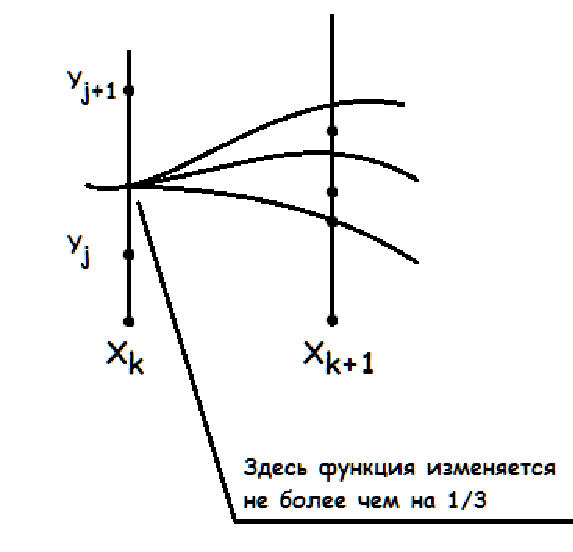
\includegraphics[width=\linewidth]{124}
\end{wrapfigure}

По лемме 2.7 $\exists\delta>0\colon\forall k\hm=1,\ldots,n\quad\forall x,y\in[a,b]\quad|x-y|<\delta$ 

$\Rightarrow$ 
$|f_k(x)-f_k(y)|<\frac\varepsilon3$

Пусть $f\in K$, тогда $\exists k\colon|f_k-f|<\frac\varepsilon3$. 

Тогда, если $|x-y|<\delta$, то $|f(x)\hm-f(y)|\le|f(x)-f_k(x)|+|f_k(x)-f_k(y)|\hm+|f_k(y)-f(y)|<\frac\varepsilon3+
\frac\varepsilon3+\frac\varepsilon3=\varepsilon$ 

$\Leftarrow$) Рассмотрим случай функций с вещественными значениями

 \noindent Пусть $c\colon\forall x\in[a,b]$, $\forall f\in K\quad |f(x)|\le c$

 Пусть задано $\varepsilon>0$. В силу равностепенной непрерывности 
 
 $\exists\delta>0\quad\forall f\in K\quad
\forall x,y\in[a,b]\colon|x-y|<\delta$ $\Rightarrow$ $|f(x)-f(y)|<\frac\varepsilon3$


Разобьем отрезок $[a,b]$ точками $\{x_k\}_{k=0}^n\colon a=x_0<x_1<\ldots<x_n=b$ так, чтобы $|x_{k+1}-x_k|<\delta$. Отрезок 
$[-c,c]$ разобьем точками $\{y_j\}_{j=0}^m$ так, чтобы $|y_{j+1}-y_j|<\frac\varepsilon3$

Рассмотрим семейство функций $\Phi$, удовлетворяющее условиям $\forall\varphi\in\Phi$:

а) $\varphi(x_0)=y_j$ для некоторых $J=0,\ldots,m$

б) если $\varphi(x_k)=y_j$, то $\varphi(x_{k+1})\in\{y_{j-1},y_j,y_{j+1}\}$

в) на $[x_k,x_{k+1}]$ $\varphi$ линейно

Семейство $\Phi$ конечно (менее $(j+1)^{k+1}$ функций). Покажем, что оно образует $\varepsilon$-сеть для $K$.

Пусть $f\in K$. Выберем $\varphi\in\Phi\colon\forall k\quad|f(x_k)-\varphi(x_k)|<\frac\varepsilon3$. 

Действительно, если $f(x_k)\in[y_j,y_{j+1}]$, то т. к. $|x_{k+1}-x_k|<\delta$, то 

$|f(x_{k+1})-f(x_k)|<\frac\varepsilon3$ $\Rightarrow$ $f(x_{k+1})\in[y_{j-1},y_{j+2}]$

$\Rightarrow$ выберем $\varphi(x_{k+1})$ ближайшим снизу к $f(x_{k+1})$, получим искомую $\varphi$

Но если $x\in[x_k,x_{k+1}]$, то $|f(x)-\varphi(x)|\le|f(x_k)-\varphi(x_k)|+|f(x)-f(x_k)|\hm+|\varphi(x)-\varphi(x_k)|\le
\frac\varepsilon3+\frac\varepsilon3+\frac\varepsilon3=\varepsilon$

$\Phi$ образует $\varepsilon$-сеть и по критерию Хаусдорфа $K$ предкомпактно $\blacksquare$
\bigskip

\noindent\textbf{Определение:} Расстоянием от точки $x_0$ до множества $A$ в метрическом пространстве $M$ называется 
$dist(x_0,A)=\inf\limits_{y\in A}\rho(x_0,y)$
\bigskip

\noindent\textbf{Определение:} Пусть $E_0$ - линейное подпространство в нормированном пространстве $E$, $\varepsilon\in[0,1)$. 
Элемент $x_\varepsilon$ называется $\varepsilon$-перпендикуляром к $E_0$, если $\|x_\varepsilon\|=1$, $dist(x_\varepsilon,
E_0)\ge1-\varepsilon$
\bigskip

\noindent\textbf{Лемма 2.8:} (Рисс) Если $E_0$ - линейное подпространство в нормированном пространстве $E$, $\bar E_0\ne E$, 
то $\forall\varepsilon\in(0,1)$ существует $\varepsilon$-перпендикуляр к $E_0$

\noindent $\square$ Выберем $x_0\in E\setminus\bar E_0$, тогда $x_0$ - внешняя точка для $E_0$, т. е. $dist(x_0,E_0)\hm=d>0$.

Возьмем $\varepsilon>0$ и выберем $y_0\in E_0\colon\|x_0-y_0\|<\frac{d}{1-\varepsilon}$

Положим $x_\varepsilon=\frac{x_0-y_0}{\|x_0-y_0\|}$

$\|x_\varepsilon\|=\frac{1}{\|x_0-y_0\|}\|x_0-y_0\|=1$

$\forall y\in E_0\quad\|x_\varepsilon-y\|=\left\|\frac{x_0-y_0}{\|x_0-y_0\|}-y\right\|=\frac{1}{\|x_0-y_0\|}\|x_0-\underbrace{
(y_0+y\|x_0-y_0\|)}_{\in E_0}\|$

$\|x_\varepsilon-y\|\ge\frac{d}{\|x_0-y_0\|}>1-\varepsilon$ $\blacksquare$
\bigskip

\noindent\textbf{Определение:} Нормы $\|\cdot\|'$ и $\|\cdot\|''$ на линейном пространстве $E$ называются эквивалентными, 
если $\exists c_1,c_2>0\colon\forall x\in E\quad c_1\|x\|'\le\|x\|''\le c_2\|x\|'$
\bigskip

Сходимость по эквивалентным нормам совпадает, фундаментальность тоже
\bigskip

\noindent\textbf{Теорема 2.4:} Любые две нормы на конечномерном пространстве эквивалентны

\noindent $\square$ Пусть $E$ - n-мерное пространство. Фиксируем базис $\{e^k\}_{k=1}^n$ и рассмотрим норму $\|x\|_2=
\left\|\sum\limits_{k=1}^n x_k r^k\right\|_2=\sqrt{\sum\limits_{k=1}^n|x_k|^2}$. Покажем, что произвольная норма $\|\cdot\|$ ей 
эквивалентна

Тогда $\|x\|=\left\|\sum\limits_{k=1}^n x_k e^k\right\|\le$(по неравенству треугольника)$\sum\limits_{k=1}^n|x_k|\cdot
\|e^k\|\le$(по неравенству Коши-Буняковского)$\|x\|_2\sqrt{\sum\limits_{k=1}^n\|e^k\|^2}=c_2\|x\|_2$

В частности $f(x)=\|x\|$ - непрерывная функция относительно евклидовой нормы, т. к. $\left|\|x\|-\|y\|\right|\le\|x-y\|$

Сфера $S=\{\|x\|_2=1\}$ компактна в $(E,\|\cdot\|_2)$ $\Rightarrow$ непрерывная функция $f$ достигает на $S$ своего минимума
$c>0$ (по 1-й аксиоме нормы), т. е. $\forall x\colon\|x\|_2=1$ выполнено $\|x\|\ge c$, т. е. $\forall x\quad\left\|
\frac{x}{\|x\|_2}\right\|\ge c$, $\|x\|\ge c\|x\|_2$ $\blacksquare$
\bigskip

\noindent\textbf{Следствие:} Если $(E,\|\cdot\|)$ - нормированное пространство, $E_0$ - конечномерное пространство, то 
$E_0$ замкнуто

\noindent $\square$ Возьмем в $E_0$ базис и зададим через него евклидову норму. По теореме 2.4 она эквивалентна исходной 
(суженной) норме

Пусть $x_n\in E_0$, $x_n\to x\in E$. Тогда $\{x_n\}$ - фундаментальная по исходной норме $\Rightarrow$ $\{x_n\}$ фундаментальная 
по евклидовой норме, в силу полноты $E_0$ по евклидовой норме $\exists x_0\in E_0\colon\|x_n-x_0\|\to0$

Тогда $\|x_n-x_0\|\to0$ $\Rightarrow$ в силу единственности предела $x_0=x$

$\Rightarrow$ $x\in E_0$ $\Rightarrow$ $E_0$ замкнуто $\blacksquare$
\bigskip

\noindent\textbf{Теорема 2.5:} Пусть $E$ - бесконечномерное нормированное пространство, $\bar B=\{x\in E\colon\|x\|\le1\}$. 
Тогда $B$ не компактно

\noindent $\square$ Построим по индукции такую последовательность $\{x_n\}$, $x_n\in B$, что $\forall n\ne k\quad\|x_n-x_k\|
\ge\frac12$

Из нее нельзя выбрать фундаментальную подпоследовательность $\Rightarrow$ $\bar B$ - не компактно

Возьмем $x_1$, $\|x_1\|=1$. Пусть $x_1,\ldots,x_n$ - построены. Положим $V_n\hm=span\{x_1,\ldots,x_n\}$(линейная оболочка). 
Тогда $V_n$ - конечномерное подпространство, $V_n$ - замкнуто $V_n=\bar V_n\ne E$

По лемме 2.8 $\exists x_{n+1}\colon\|x_{n+1}\|=1$, $dist(x_{n+1},V_n)>\frac12$. По определению $dist$ $\forall y\in V_n
\quad\|x_{n+1}-y\|>\frac12$, в частности, $\forall k\le n\quad\|x_{n+1}-x_k\|>\frac12$

По индукции получаем искомую последовательность $\blacksquare$
\bigskip
\bigskip

\noindent\textbf{Было:} непрерывные функции с нормой

$$\|f\|_1=\displaystyle\int\limits_{[0,1]}|f(x)|dx$$

$$\|f\|_2=\sqrt{\displaystyle\int\limits_{[0,1]}|f(x)|^2dx}$$

\noindent A) Как построить пополнение:

1) пополнение в виде пространства последовательностей

2) более широкое пространство функций с той же метрикой

Интеграла Римана недостаточно, все непрерывные функции образуют неполное пространство, более общий интеграл Лебега дает 
полное пространство

\noindent Б) Задача о разложении в ряд Фурье

$f\colon a_n(f)=\frac1\pi\displaystyle\int\limits_{-\pi}^\pi f(x)\cos\pi x dx$

Чем общее интеграл, тем больше функций можно разлагать

\noindent Основная идея инетгралов:

Риман: $\Delta k=\{x\colon x_{k-1}<x<x_k\}$

$S_T(f)=\sum f(\xi_k)\cdot|\Delta k|$

Лебег: $S_T(f)=\sum f(\xi_k)|\Delta k|$

$\Delta k=\{x\colon y_{k-1}\le f(x)<y_k\}$, $\xi_k\in\Delta k$








\chapter{Системы множеств}

\noindent\textbf{Определение:} Система множеств $S$ называется полукольцом, если:

1) $\varnothing\in S$

2) $\forall A,B\in S\quad A\cap B\in S$

3) если $A\in S$, $A_1\in S$, $A_1\subset A$, то $\exists A_2,\ldots,A_n\in S\colon A=\bigsqcup\limits_{k=1}^n A_k$ 

($A=\bigcup\limits_{k=1}^n A_k\colon A_k\cap A_j=\varnothing$, $k\ne j$)
\bigskip

\noindent\textbf{Определение:} Система множеств $R$ называется кольцом, если:

1) $\varnothing\in R$

2) $\forall A,B\in R\quad A\cup B\in R$

3) $\forall A,B\in R\quad A\triangle B\in R$

($A\triangle B=(A\setminus B)\cup(B\setminus A)$)
\bigskip

\noindent\textbf{Определение:} Множество $X$ называется единицей системы $S$, если $X\in S$ и $\forall A\in S$ выполняется
$A\subset X$
\bigskip

\noindent\textbf{Определение:} Кольцо с единицей называется алгеброй
\bigskip

\noindent\textbf{Определение:} Кольцо (алгебра) называется $\sigma$-кольцом ($\sigma$- алгеброй), если $\forall\{A_k\}$, 
$A_k\in R$ выполнено $\bigcup\limits_{k=1}^\infty A_k\in R$
\bigskip

\noindent\textbf{Пример:} $S=\{[a,b],[a,b),(a,b],(a,b)|\quad\alpha\le a\le b\le\beta\}$
\bigskip

\noindent Свойства полукольца:

1) $\varnothing=(a,a)$

2) пересечение - промежуток или пусто

3) выполнено при $n\le3$

$[\alpha,\beta]$ - единица $\Rightarrow$ $S$ - не кольцо
\bigskip

\noindent Примеры полуколец:

1) $X$ - любые; $R_1=\{\varnothing,X\}$; $R_2$ - все подмножества $X$;

$R_1$, $R_2$ - $\sigma$-алгебры с единицей $X$

2) $S=\{I_1\times I_2|\quad I_1,I_2$ - промежутки на $\mathbb R\}$
\bigskip

\noindent\textbf{Лемма 3.1:} Всякое кольцо является полукольцом

\noindent $\square$ Пусть $A,B\in R$, тогда $A\cap B=(A\cup B)\triangle(A\triangle B)\in R$

$A\setminus B=(A\triangle B)\cap A\in R$ $\Rightarrow$ если $A,A_1\in R$, $A_1\in A$, то при $A_2=A\setminus A_1$ имеем: 
$A=A_1\sqcup A_2$ $\blacksquare$
\bigskip

\noindent\textbf{Лемма 3.2:} Пусть $S$ - полукольцо, $A,A_1,\ldots,A_n\in S$, $A\supset\bigsqcup\limits_{k=1}^n A_k$. 
Тогда $\exists A_{n+1},\ldots,A_l\in S\colon A=\bigsqcup\limits_{k=1}^l A_k$

\begin{wrapfigure}[10]{L}{0.3\linewidth} 
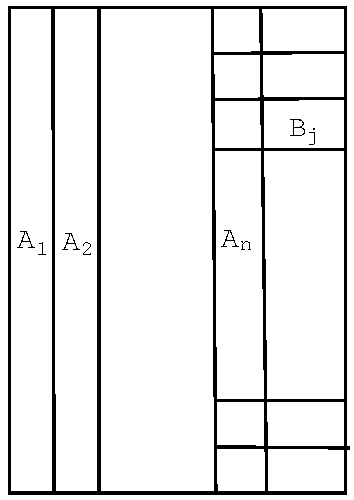
\includegraphics[width=\linewidth]{3}
\end{wrapfigure}

\noindent $\square$ По индукции по n

При $n=1$ - по 3-й аксиоме полукольца

Пусть верно для $(n-1)$ множеств и даны $A_1,\ldots,A_n\in S\colon A\supset\bigsqcup\limits_{k=1}^n A_k$

\noindent Тогда по предположению индукции $\exists B_1,\ldots,B_s\hm\in S\colon A=\bigsqcup\limits_{k=1}^{n-1}A_k\sqcup\bigsqcup\limits
_{j=1}^s B_j$, тогда $A_n\subset\bigsqcup\limits_{j=1}^s B_j$

Пусть $C_j=A_n\cap B_j\in S$, тогда $A_n=\bigsqcup\limits_{j=1}^s C_j$, но $C_j\subset B_j$

По 3-й аксиоме полукольца $\exists D_{i,j}\in S$,

 $i=1,\ldots,i_j\colon B_j=C_j\sqcup\left(\bigsqcup\limits_{j=1}^{i_j}
D_{i,j}\right)$

Тогда $A=\bigsqcup\limits_{k=1}^{n-1}A_k\sqcup\bigsqcup\limits_{j=1}^s\left(C_j\sqcup\bigsqcup\limits_{i=1}^{i_j} D_{i,j}\right)=
\bigsqcup\limits_{k=1}^n A_k\sqcup\left(\bigsqcup\limits_{j=1}^s\bigsqcup\limits_{i=1}^{i_j}D_{i,j}\right)$ $\blacksquare$
\bigskip

\noindent\textbf{Лемма 3.3:} Пусть $S$ - полукольцо, $A_1,\ldots,A_n\in S$. Тогда $\exists\{B_j\}_{j=1}^k$ - попарно 
непересекающиеся элементы $S\colon$ каждые $A_i$ есть объединение некоторых $B_j$

\noindent $\square$ По индукции по n

При $n=1$ утверждение тривиально

Пусть для $(n-1)$ множества утверждение доказано, и даны $A_1,\ldots,A_n$. Пусть $\{B_j\}$ - набор для $A_1,\ldots,A_{n-1}$
из условия леммы

Положим $C_j=B_j\cap A_n\in S$

По 3-й аксиоме $\exists D_{i,j}\in S\colon B_j=C_j\sqcup\bigsqcup\limits_i D_{i,j}$

Поскольку $A_n\supset\bigsqcup\limits_{j=1}^k C_j$, то по лемме 3.2 $\exists E_l\in S$, $l=1,\ldots,L\colon $

$A_n=\bigsqcup
\limits_{j=1}^k C_j\sqcup\bigsqcup\limits_{l=1}^L E_l$

Тогда система $\{C_j,D_{i,j},E_l\}$ - искомая для $A_1,\ldots,A_n$

$\left(\forall s<n\quad A_s=\bigsqcup\limits_{\text{по некот. }j}B_j=\bigsqcup\limits_{\text{по некот. }j}(C_j\sqcup
\bigsqcup\limits_{i=1}^{i_j}D_{i,j})\right)$ $\blacksquare$
\bigskip

\noindent\textbf{Определение:} Кольцо (алгебра, $\sigma$-алгебра) $R$ называется наименьшим кольцом (алгеброй, $\sigma$-алгеброй), 
содержащим систему множеств $S$, если $\forall$ кольца (алгебры, $\sigma$-алгебры) $R_1$ из условия $R_1\supset S$ 
следует, что $R_1\supset R$
\bigskip

\noindent\textbf{Теорема 3.1:} Пусть $S$ - полукольцо. Тогда наименьшее содержащее его кольцо $R=R(S)$ есть $R(S)=\left\{
\bigcup\limits_{j=1}^n A_j|\quad A_j\in S\right\}=\left\{\bigsqcup\limits_{j=1}^l B_j|\quad B_j\in S\right\}$

\noindent $\square$ 1) Второе равенство следует из леммы 3.3 (если каждое $A_j$ есть объединение некоторых $B_k$, то 
$\bigcup\limits_{j=1}^n A_j=\bigsqcup\limits_k B_k$)

2) Если $R_1$ - кольцо, $R_1\supset S$, то $R_1\supset R(s)$ по 2-й аксиоме кольца

3) Проверим, что $R$ - кольцо

$\varnothing\in S\subset R$; Если $A',A''\in R$, то $A'\cup A''=\left(\bigcup\limits_k A_k'\right)\cup\left(\bigcup\limits_l
A_l''\right)\in R(S)$, где $A_k'\in S$, $A_l''\in S$

Пусть теперь $A,B\in R$, $A=\bigsqcup\limits_{k=1}^n A_k$, $B=\bigsqcup\limits_{j=1}^l B_j$, $A_k\in S$, $B_j\in S$

Тогда $A\setminus B=\left(\bigsqcup\limits_{k=1}^n A_k\right)\setminus\left(\bigsqcup\limits_{j=1}^l B_j\right)=
\bigsqcup\limits_{k=1}^n\left(A_k\setminus\bigsqcup\limits_{j=1}^l(B_j\cap A_k)\right)\stackrel{\text{л.3.2}}{=}$

\noindent$=\bigsqcup\limits_{k=1}^n\bigsqcup\limits_{i=1}^{i_k}C_{i,k}$, где $C_{i,k}\in S$

Наконец $\forall A',A''\in R(S)\quad A'\triangle A''=(A'\setminus A'')\cup(A''\setminus A')\in R(S)$ $\blacksquare$







\chapter{Меры на полукольцах и кольцах}

\noindent\textbf{Определение:} Пусть $S$ - полукольцо. Функция $m\colon S\to[0;+\infty)$ или $m\colon S\to[0;+\infty)\cup
\{+\infty\}$ называется мерой, если $\forall A\in S$, $\forall A_1,\ldots,A_n\in S$ таких, что $A=\bigsqcup\limits_{k=1}^n
A_k$ выполнено равенство $mA=\sum\limits_{k=1}^n mA_k$

Мера называется $\sigma$-аддитивной (счетно-аддитивной), если $\forall A\in S$, 

\noindent $A_k\in S$ таких, что $A=\bigsqcup\limits_{k=1}^\infty A_k$ выполнено равенство $mA=\sum\limits_{k=1}^\infty mA_k$
\bigskip

\noindent\textbf{Замечание:} $\sum\limits_{k=1}^\infty mA_k=\infty$ $\Rightarrow$ $\exists k\colon mA_k=\infty$

$\sum\limits_{k=1}^\infty mA_k=+\infty$ $\Leftrightarrow$ $\exists k\colon mA_k=+\infty$ или ряд расходится
\bigskip

\noindent Примеры:

1. $S$ - полукольцо промежутков $m[a,b]=[a,b)=m(a,b]=m(a,b)=b-a$ (стандартная мера на полукольце промежутков)

\begin{wrapfigure}[2]{r}{0.5\linewidth} 
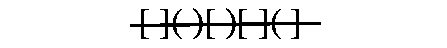
\includegraphics[width=\linewidth]{4}
\end{wrapfigure}
 
Расставим по порядку:

\noindent
$a_1\le b_1\le a_2\le b_2\le\ldots\le a_n\le b_n$

Если $b_k<a_{k+1}$, то $A\ne\bigsqcup\limits_k A_k$ $\Rightarrow$ $b_k=a_{k+1}$ 

$\Rightarrow$ тогда $\sum\limits_k
(b_k-a_k)=(b_k-a_1)$

2. $S$ - полукольцо промежутков, $\varphi$ - неубывающая непрерывная функция

$m_\varphi[a,b]=m_\varphi[a,b)=m_\varphi(a,b]=m_\varphi(a,b)=\varphi(b)-\varphi(a)$ (мера Стилтьеса)
\bigskip

3. Дискретные меры

$X$ - множество, $R$ - $\sigma$-алгебра всех его подмножеств, $X_k$ - точки из $X$ (конечный или счетный набор) 
$a_k\ge0$, $\forall A\subset X\quad mA=\sum\limits_{k\colon X_k\in A}a_k$

Тогда $m$ - $\sigma$-аддитивная мера
\bigskip

\noindent\textbf{Теорема 4.1:} Пусть $m$ - мера на полукольце $S$. Тогда существует единственное ее продолжение до меры на 
$R(S)$ (обычно обозначается той же буквой)

\noindent $\square$ Пусть $m$ - мера на $S$. $A\in R(S)$, по т. 3.1 $\exists A_k\in S$, $A=\bigsqcup_{k=1}^n A_k$. 
Тогда $mA\stackrel{def}{=}\sum\limits_{k=1}^n mA_k$ - единственно возможное продолжение 

Корректность: пусть к тому же $\exists B_j\in S\colon A=\bigsqcup\limits_{j=1}^l B_j$

Положим $C_{k,j}=A_k\cap B_j\in S$. Тогда $A_k=\bigsqcup\limits_{j=1}^l C_{k,j}$, $B_j=\bigsqcup\limits_{k=1}^n C_{k,j}$

Тогда $\sum\limits_{k=1}^n mA_k=\sum\limits_{k=1}^n\left(\sum\limits_{j=1}^l mC_{k,j}\right)=\sum\limits_{j=1}^l
\left(\sum\limits_{k=1}^n mC_{k,j}\right)=\sum\limits_{j=1}^l mB_j$

Пусть $C,C_k\in R(S)$, $C=\bigsqcup\limits_{k=1}^n C_k$

$\exists A_{k,j}\in S\colon C_k=\bigsqcup\limits_{j=1}^k A_{k,j}$ тогда $C=\bigsqcup\limits_{k=1}^n\bigsqcup\limits_{j=1}^{j_k}
A_{k,j}$

$mC=\sum\limits_{k=1}^n\sum\limits_{j=1}^{j_k}mA_{k,j}=\sum\limits_{k=1}^n mC_k$ $\blacksquare$
\bigskip

\noindent\textbf{Теорема 4.2:} Пусть $m$ - $\sigma$-аддитивная мера на полукольце $S$. Тогда ее продолжение на минимальное 
кольцо $R(S)$ - $\sigma$-аддитивная мера

\noindent $\square$ Пусть $A\in R(S)$, $A_n\in R(S)$, $A=\bigsqcup\limits_{n=1}^\infty A_n$

$\exists C_k\in S\colon A=\bigsqcup\limits_{k=1}^l C_k$, $\exists B_{n,j}\in S\colon A_n=\bigsqcup\limits_{j=1}^{j_n} B_{n,j}$
(по теореме 3.1)

Положим $D_{k,n,j}=C_k\cap B_{n,j}\in S$, тогда $C_k=\left(\bigsqcup\limits_n\bigsqcup\limits_{j=1}^{j_n} B_{n,j}\right)\cap C_k\hm=
\bigsqcup\limits_{n=1}^\infty\bigsqcup\limits_{j=1}^{j_m} D_{k,n,j}$

$mC_k=\sum\limits_{n=1}^\infty\sum\limits_{j=1}^{j_n}mD_{k,n,j}$

С другой стороны, $B_{n,j}=\bigsqcup\limits_{k=1}^l D_{k,n,j}$, т. е. $mB_{n,j}=\sum\limits_{k=1}^l mD_{k,n,j}$

Тогда $mA=\sum\limits_{k=1}^l mC_k=\sum\limits_{k=1}^l\sum\limits_{n=1}^\infty\sum\limits_{j=1}^{j_n} mD_{k,n,j}=
\sum\limits_{n=1}^\infty\sum\limits_{j=1}^{j_n}\left(\sum\limits_{k=1}^l mD_{k,n,j}\right)\hm=\sum\limits_{n=1}^\infty
\sum\limits_{j=1}^{j_n}mB_{n,j}=\sum\limits_{n=1}^\infty mA_n$ $\blacksquare$
\bigskip

\noindent\textbf{Теорема 4.3:} Пусть $m$ - мера на полукольце $S$

(a) Если $A_n\in S$, $A\in S$, $\bigsqcup\limits_n A_n\subset A$, то $\sum\limits_n mA_n\le mA$

(б) Если $A_n\in S$, $A\in S$, $A\subset\bigcup\limits_{n=1}^N A_n$, то $mA\le\sum\limits_{n=1}^N mA_n$

\noindent $\square$ (а) Если $\bigsqcup\limits_{n=1}^N A_n\subset A$, то по лемме 3.1 $\exists A_{N+1},\ldots,A_M\in S\colon
A=\bigsqcup\limits_{n=1}^M A_n$

По определению меры $mA=\sum\limits_{n=1}^M mA_n\ge\sum\limits_{n=1}^N mA_n$. Если же $\bigsqcup\limits_{n=1}^\infty A_n\subset
A$, то $\forall N\quad\bigsqcup\limits_{n=1}^N A_n\subset A$, по доказанному $\sum\limits_{n=1}^N mA_n\le mA$.

При $N\to\infty$ в пределе $\sum\limits_{n=1}^\infty mA_n\le mA$

(б) Пусть даны $A$ и $A_n$. По лемме 4.2 $\exists$ попарно непересекающиеся $B_j\in S$ и конечные множества $P_n\subset
\mathbb N$, $n=0,1,\ldots,N\colon A=\bigsqcup\limits_{j\in P_0}B_j$, $A_n=\bigsqcup\limits_{j\in P_n}B_j$

Т. к. $A\subset\bigcup\limits_{n=1}^N A_n$, то $\forall j\in P_0\quad\exists n\le1\colon j\in P_n$

$mA=\sum\limits_{n=1}^N\left(\sum\limits_{j\in P_n}mB_j\right)=\sum\limits_{n=1}^N mA_n$
(каждое слагаемое в левой сумме хотя бы раз входит в правую) $\blacksquare$
\bigskip

\noindent\textbf{Теорема 4.4:} Пусть $m$ - мера на полукольце $S$. $m$ $\sigma$-аддитивна т. и т. т. к. $\forall A,A_n\in S$
таких, что $A\subset\bigcup\limits_{n=1}^\infty A_n$ выполнено неравенство $A\le\sum\limits_{n=1}^\infty mA_n$

\noindent $\square$ $(\Leftarrow)$ Пусть $A,A_n\in S$, $A=\bigsqcup\limits_{n=1}^\infty A_n$

$A\supset\bigcup\limits_{n=1}^\infty A_n$ $\Rightarrow$ $mA\le\sum\limits_{n=1}^\infty mA_n$ по т. 4.3(а)

$A\subset\bigcup\limits_{n=1}^\infty A_n$ $\Rightarrow$ $mA\le\sum\limits_{n=1}^\infty mA_n$ по условию $mA=\sum\limits_{n=1}^\infty
mA_n$, $m$ $\sigma$-аддитивная

$(\Rightarrow)$ Продолжим меру $m$ на кольцо $R(S)$. По т. 4.2 получим $\sigma$-аддитивную меру

Пусть $A\subset\bigcup\limits_{n=1}^\infty A_n$, $A,A_n\in S$. Рассмотрим $B_n=\left(A_n\setminus\bigcup\limits_{k=1}^{n-1}
A_k\right)\cap A\hm\in R(S)$

Тогда $A=\bigsqcup\limits_{n=1}^\infty B_n$ ($\forall x\in A\quad\exists$ минимальное $n\colon x\in A_n$, тогда $x\in B_n$)

В силу $\sigma$-аддитивности $mA=\sum\limits_{n=1}^\infty mB_n\le\sum\limits_{n=1}^\infty mA_n$ $\blacksquare$
\bigskip

\noindent\textbf{Определение:} Мера $m$ на полукольце $S$ называется непрерывной снизу, если $\forall A,A_n\in S$ таких, 
что $A_n\subset A_{n+1}$, $A=\bigcup\limits_{n=1}^\infty A_n$ выполнено 

$mA=\lim\limits_{n\to\infty}mA_n$
\bigskip

\noindent\textbf{Определение:} Мера $m$ на полукольце $S$ называется непрерывной сверху, если $\forall A,A_n\in S$ таких, 
что $A_n\supset A_{n+1}$, $A=\bigcap\limits_{n=1}^\infty A_n$ выполнено 

$mA=\lim\limits_{n\to\infty}mA_n$
\bigskip

\noindent\textbf{Теорема 4.5:} Мера $m$ на кольце $R$ $\sigma$-аддитивна т. и т. т. к. $m$ непрерывна снизу

\noindent $(\Rightarrow)$ Пусть $A,A_n\in R$, $A_n\subset A_{n+1}$, $A=\bigcup\limits_{n=1}^\infty A_n$. Положим $B_1=A_n$,

\noindent$B_n=A_n\setminus A_{n-1}\in R$ $(n\ge2)$

Тогда $\forall n\quad A_n=\bigsqcup\limits_{k=1}^n B_k$, $A=\bigsqcup\limits_{k=1}^\infty B_k$

По определению суммы ряда $mA=\sum\limits_{k=1}^\infty mB_k=\lim\limits_{n\to\infty}\sum\limits_{k=1}^n mB_k=\lim
\limits_{n\to\infty}mA_n$

$(\Leftarrow)$ Пусть $A=\bigsqcup\limits_{n=1}^\infty B_k$, $B_k\in R$, $A\in R$. Положим $A_n=\bigsqcup\limits_{k=1}^n B_k$, 
тогда $A_n\in R$, $mA_n=\sum\limits_{k=1}^n mB_k$, $A_n\subset A_{n+1}$

$A=\bigcup\limits_{k=1}^\infty A_n$. Тогда $mA=\lim\limits_{n\to\infty}mA_n=\lim\limits_{n\to\infty}\sum\limits_{k=1}^n mB_k=
\sum\limits_{k=1}^\infty mB_k$ $\blacksquare$
\bigskip

\noindent\textbf{Следствие:} (a) Пусть $m$ $\sigma$-аддитивная мера на кольце $R$, $A_n,A\in R$, 

\noindent $A_n\supset A_{n+1}$, $A=\bigcap\limits_{n=1}^\infty A_n$ и $mA_1<\infty$ (тогда $\forall n\quad mA_n<+\infty$)

Тогда $mA=\lim\limits_{n\to\infty} mA_n$

(б) Конечная $\sigma$-аддитивная мера на кольце непрерывна сверху

\noindent $\square$ (а) Положим $B_n=A_1\setminus A_n$, $B=A_1\setminus A$. Тогда $B_n\in R$, $B\in R$, $B_n\subset B_{n+1}$

$B=A_1\setminus\left(\bigcap\limits_{n=1}^\infty A_n\right)=\bigcup\limits_{n=1}^\infty\left(A_1\setminus A_n\right)=
\bigcup\limits_{n=1}^\infty B_n$

По т. 4.5 $m B=\lim\limits_{n\to\infty} mB_n$

$A_1=A_n\sqcup B_n=B\sqcup A$

$mA_1=mA_n+mB_n=mB+mA$

$mA_1-mA_n=mB_n$

$mA_1-mA=mB$

$mA_1-mA=\lim\limits_{n\to\infty}(mA_1-mA_n)$ $\Rightarrow$ $mA=\lim\limits_{n\to\infty} mA_n$

(б) Следует из (а), т. к. в случае конечной меры $A_1<+\infty$ для любой последовательности такого вида $\blacksquare$
\bigskip

\noindent\textbf{Теорема 4.6:} Стандартная мера на полукольце промежутков в $\mathbb R$ $\sigma$-аддитивна

\noindent $\square$ По т. 4.3(а) достаточно доказать, что если $I=\bigsqcup\limits_{n=1}^\infty I_n$, $I,I_n\in S$, то 

$mI\le\sum\limits_{n=1}^\infty mI_n$

Пусть в начале $I$ - конечный промежуток с концами a и b

$\forall\varepsilon>0\quad\exists[a',b']\in I\colon mI-m[a',b']<\frac\varepsilon2$ и $\forall n\quad\exists$ интервал 
$J_n\supset I_n\colon$ 

$mJ_n-mI_n<\displaystyle\frac{\varepsilon}{2^{n+1}}$

Тогда $[a',b']\subset\bigcup\limits_{n=1}^\infty J_n$. Тогда $\exists N\colon[a',b']\subset\bigcup\limits_{n=1}^N J_n$

По т. 4.3(б) $m[a',b']\le\sum\limits_{n=1}^N mJ_n$

$mI-\frac\varepsilon2\le\sum\limits_{n=1}^N\left(mI_n+\displaystyle\frac{\varepsilon}{2^{n+1}}\right)\le\sum\limits_{n=1}^\infty mI_n
+\sum\limits_{n=1}^\infty\displaystyle\frac{\varepsilon}{2^{n+1}}=\sum\limits_{n=1}^\infty mI_n+\frac\varepsilon2$

$mI\le\sum\limits_{n=1}^\infty mI_n+\varepsilon$, где $\varepsilon>0$ - любое; $mI\le\sum\limits_{n=1}^\infty mI_n$

Пусть $I$ - бесконечный промежуток. Если $\exists n\colon I_n$ - бесконечен, то утверждение верно. 

Предположим, что все $I_n$ конечны и $\sum\limits_{n=1}^\infty mI_n=C<+\infty$

$\exists N\colon mI\cap[-N;N]>C+1$

$I\cap[-N,N]=\bigsqcup\limits_{n=1}^\infty I_n\cap[-N,N]$, где $\sum\limits_{n=1}^\infty m\left(I_n\cap[-N,N]\right)\le
\sum\limits_{n=1}^\infty mI_n<C$

 $m\left(I\cap[-N,N]\right)>C+1$, что противоречит уже разобранному случаю $\blacksquare$

 
 
 
 
 
 
 
 
\chapter{Продолжение меры по Лебегу}

Далее $S$ - полукольцо с единицей $X$, $m$ $\sigma$-аддитивная мера на $S$, причем $mX<+\infty$
\bigskip

\noindent\textbf{Определение:} Внешней мерой Лебега множества $A\subset X$ называется 

$\mu^*A=\inf\limits_{\{A_k\}\colon A_k\in S}\sum\limits_k mA_k$, $A\in\bigcup\limits_k A_k$ - конечные или счетные покрытия

$\forall A\subset X\colon\mu^*A$ определена и конечна
\bigskip

\noindent\textbf{Теорема 5.1:} Если $A\subset X$, $A_n\subset X$, $A\subset\bigcup\limits_n A_n$, то $\mu^*A\le
\sum\limits_n\mu^*A_n+\displaystyle\frac{\varepsilon}{2^n}$

\noindent $\square$ Пусть $\varepsilon>0$. $\forall n\quad\exists I_{n,k}\in S\colon A_n\subset\bigcup\limits_k I_{n,k}$
и $\sum\limits_k mI_{n,k}<\mu^*A_n+\displaystyle\frac{\varepsilon}{2^n}$

Но тогда $A\subset\bigcup\limits_n\bigcup\limits_k I_{n,k}$; тогда по определению $\mu^*A\le\sum\limits_n\sum\limits_k
mI_{n,k}\hm<\sum\limits_n\left(\mu^*A_n+\displaystyle\frac{\varepsilon}{2^n}\right)<\left(\sum\limits_n\mu^* A_n\right)+\varepsilon$, 
где $\varepsilon>0$ - любое

$\Rightarrow$ $A\le\sum\mu^*A_n$ $\blacksquare$
\bigskip

\noindent\textbf{Следствие:} Если $A\subset X$, $B\subset X$, то $|\mu^*A-\mu^*B|\le\mu^*(A\triangle B)$

\noindent $\square$ $A\subset B\cup(A\triangle B)$

$B\subset A\cup(A\triangle B)$

$\mu^*A\le\mu^*B+\mu^*(A\triangle B)$

$\mu^*B\le\mu^*A+\mu^*(A\triangle B)$ $\blacksquare$
\bigskip

\noindent\textbf{Замечание:} $\mu^*$ вообще говоря не является мерой на $\sigma$-алгебре всех подмножеств в $X$
\bigskip

\noindent\textbf{Определение:} Множество $A\subset X$ назывется измеримым (по Лебегу), если $\forall\varepsilon>0\quad
\exists B_\varepsilon\in R(S)\colon\mu^*(A\triangle B_\varepsilon)<\varepsilon$ $(A\in\mathfrak M)$
\bigskip

\noindent\textbf{Определение:} Мерой Лебега измеримого множества называется его внешняя мера $\mu A=\mu^*A$
\bigskip
\bigskip
\bigskip

\noindent\textbf{Лемма 5.1:} (а) Если $\mu^*A=0$, то $A\in\mathfrak M$

(б) Если $A\in R(S)$, то $A\in\mathfrak M$ и $\mu A=\mu^*A=mA$

\noindent $\square$ (а) $\forall\varepsilon>0$ возьмем $B_\varepsilon=\varnothing\in R(S)$. Тогда $\mu^*(A\triangle B_\varepsilon)=
\mu^*A=0<\varepsilon$

(б) $\forall\varepsilon>0$ возьмем $B_\varepsilon=A$. Тогда  $\mu^*(A\triangle A)=\mu^*\varnothing=0$ $\Rightarrow A\in\mathfrak M$

Если $A\subset\bigcup\limits_n I_n$, $I_n\in S$, то $mA\le\sum\limits_n mI_n$, по т. 4.4 (мера $m$ $\sigma$-аддитивная)

$\Rightarrow$ $mA\le\mu^*A=\mu A$

Обратно, т. к. $A=\bigsqcup\limits_{k=1}^n B_k$, $B_k\in S$, то по т. 4.1 $mA=\sum\limits_{k=1}^n mB_k\ge\mu^*A$ 

(т. к. $\bigsqcup\limits_k B_k$ - одно из возможных покрытий $A$ элементами $S$) $\blacksquare$
\bigskip

\noindent\textbf{Определение:} Мера $m$ на полукольце $S$ называется полной, если 

$\forall A\in S\colon mA=0$ и 
$\forall B\subset A$ выполнено, что $B\in S$ (тогда $mB=0$, т. к. $mB\le mA$)
\bigskip

\noindent\textbf{Следствие:} Мера Лебега полна

\noindent $\square$ Если $A\in\mathfrak M$, $\mu A=0$, $B\subset A$, то по т. 5.1 $\mu^*B\le\mu^*A=\mu^*B=0$ $\Rightarrow$
по л. 5.1 $B\in\mathfrak M$ $\blacksquare$
 \bigskip
 
 \noindent\textbf{Теорема 5.2:} Система измеримых множеств $\mathfrak M$ является алгеброй
 
\noindent $\square$ (1) $X\in\mathfrak M$ по л. 5.1(б)

(2) Пусть $A_1,A_2\in\mathfrak M$, $\varepsilon>0$

$\exists B_1,B_2\in R(S)\colon\mu^*(A_k\triangle B_k)<\frac\varepsilon2$; $k=1,2$

Заметим, что $(A_1\cup A_2)\triangle(B_1\cup B_2)\subset(A_1\triangle B_1)\cup(A_2\triangle B_2)$ $(*)$

По т. 5.1 $\mu^*\left((A_1\cup A_2)\triangle(B_1\cup B_2)\right)\le\mu^*(A_1\triangle B_1)+\mu^*(A_2\triangle B_2)<\frac\varepsilon2
+\frac\varepsilon2=\varepsilon$

Но $B_1\cup B_2\in R(S)$ $\Rightarrow$ $A_1\cup A_2\in\mathfrak M$

(3) Если $A\in\mathfrak M$, $B\in R(S)$, то $X\setminus B\in R(S)$ и $A\triangle B=(X\setminus A)\triangle(X\setminus B)$ 
$\Rightarrow$ $X\setminus A\in\mathfrak M$. Если $A_1,A_2\in\mathfrak M$, то

$A_1\cap A_2=x\setminus\left((X\setminus A_1)\cup(X\setminus A_2)\right)\in\mathfrak M$

$A_1\setminus A_2=A_1\cap(X\setminus A_2)\in\mathfrak M$

$A_1\triangle A_2=(A_1\setminus A_2)\cup(A_2\setminus A_1)\in\mathfrak M$ $\blacksquare$
\bigskip

\noindent\textbf{Теорема 5.3:} Мера Лебега $\mu$ есть $\sigma$-аддитивная мера на $\mathfrak M$

\noindent $\square$ (1) Докажем, что $\mu$ - мера. Пусть $A_1,A_2\in\mathfrak M$, $A_1\cap A_2=\varnothing$

$\exists B_1,B_2\in R(S)\colon\mu^*(A_k\triangle B_k)<\varepsilon$

Тогда в силу (*) $\mu^*\left((A_1\cup A_2)\triangle (B_1\cup B_2)\right)<2\varepsilon$

По следствию из т. 5.1 $|\mu^*A_k-\mu^*B_k|=|\mu A_k-\mu B_k|<\varepsilon$

$|\mu^*(A_1\cup A_2)-\mu^*(B_1\cup B_2)|=|\mu(A_1\cup A_2)-m(B_1\Cup B_2)|<2\varepsilon$

Заметим, что т.к $A_1\cap A_2=\varnothing$, то $B_1\cap B_2\subset(A_1\triangle B_1)\cup(A_2\triangle B_2)$

Поэтому $m(B_1\cap B_2)=\mu^*(B_1\cap B_2)\le\mu^*(A_1\triangle B_1)+\mu^*(A_2\triangle B_2)<2\varepsilon$

Т.к. $m$ - мера на $R(S)$, то $mB_1+mB_2=m(B_1\setminus B_2)+m(B_1\cap B_2)+m(B_2\hm\setminus B_1)+m(B_1\cap B_2)=
m(B_1\cup B_2)+m(B_1\cap B_2)$

Надо доказать, что $\mu(A_1\sqcup A_2)=\mu A_1+\mu A_2$ 

По т. 5.1 $\mu(A_1\sqcup A_2)\le\mu A_1+\mu A_2$

Обратно, $\mu(A_1\sqcup A_2)\ge m(B_1\cup B_2)-2\varepsilon=m(B_1)+m(B_2)-m(B_1\cap B_2)-2\varepsilon\ge$

\noindent$\ge mB_1+mB_2-4\varepsilon\ge\mu A_1+\mu A_2-6\varepsilon$

Т. к. $\varepsilon>0$ - любое, то $\mu(A_1\sqcup A_2)\ge \mu A_1+\mu A_2$. Т. к. $\mathfrak M$ - алгебра, то по индукции
$\forall n\quad\mu(\bigsqcup\limits_{k=1}^n A_k)=\sum\limits_{k=1}^k\mu A_k$

(2) По т. 4.4 $\sigma$-аддитивность меры эквивалентна тому, что если 

$A\subset\bigcup\limits_{n=1}^\infty A_n$, то 
$\mu A\le\sum\limits_{n=1}^\infty \mu A_n$. Но для меры Лебега это неравенство верно по т. 5.1 $\blacksquare$
\bigskip

\noindent\textbf{Теорема 5.4:} Система измеримых множеств $\mathfrak M$ является $\sigma$-алгеброй

\noindent $\square$ Пусть $A=\bigcup\limits_{n=1}^\infty A_n$, $A_n\in\mathfrak M$. Т. к. $\mathfrak M$ - алгебра, то 
$B_n=A_n\setminus\bigcup\limits_{k=1}^{n-1} A_k\in\mathfrak M$ и $A=\bigsqcup\limits_{n=1}^\infty B_n$

Тогда по т. 5.3 и 5.2 $\forall N\quad\mu^*A\ge\mu^*(\bigsqcup\limits_{n=1}^N B_n)=\mu(\bigsqcup\limits_{n=1}^N B_n)=
\sum\limits_{n=1}^N\mu B_n$, т.е. $\sum\limits_{n=1}^\infty \mu B_n<+\infty$

Пусть задано $\varepsilon>0$. Зафиксируем $N$ так, чтобы $\sum\limits_{n=N+1}^\infty\mu B_n<\frac\varepsilon 2$. 

Положим $C=\bigsqcup\limits_{n=1}^N B_n$, $D=\bigsqcup\limits_{n=N+1}^\infty B_n$, $A=C\sqcup D$

Тогда по т. 5.2 $C\in\mathfrak M$, по т. 5.1 $\mu^*D\le\sum\limits_{n=N+1}^\infty\mu B_n<\frac\varepsilon2$

Тогда $\exists C_\varepsilon\in R(S)\colon\mu^*(C\triangle C_\varepsilon)<\frac\varepsilon 2$. Тогда $A\triangle C_\varepsilon\subset
(C\triangle C_\varepsilon)\cup D$ и по т. 5.1 $\mu^*(A\triangle C_\varepsilon)\le\mu^*(C\triangle C_\varepsilon)+\mu^*D<
\frac\varepsilon2+\frac\varepsilon2=\varepsilon$

$\Rightarrow$ $A\in\mathfrak M$ по определению $\blacksquare$
\bigskip

\noindent\textbf{Пример:} Стандартная мера на полукольце промежутков $[A,B]$

Если $G$ - открытое, то $G=\bigcup\limits_{n=1}^\infty(a_n,b_n)\in\mathfrak M$

Если $F$ - замкнутое, то $F=X\setminus(X\setminus F)\in\mathfrak M$
\bigskip

\noindent\textbf{Определение:} Мера $m$ на полукольце $S$ с единицей $X$ называется $\sigma$-конечной, если $\exists 
X_n\in S\colon mX_n<+\infty$, $X=\bigsqcup\limits_{n=1}^\infty X_n$, $mX=+\infty$
\bigskip

\noindent\textbf{Пример:} $m$ - стандартная мера на всех промежутках прямой 

$\mathbb R=\bigsqcup\limits_{n\in\mathbb Z}[n,n+1)$
\bigskip

\noindent\textbf{Определение:} Пусть $m$ - $\sigma$-конечная мера на полукольце  $S$ с единицей $X$, $X=\bigsqcup
\limits_{n=1}^\infty X_n$, $X_n\in S$, $mX_n<+\infty$

Множество $A\subset X$ называется измеримым по Лебегу, если $\forall n\quad A\cap X_n$ измеримо по Лебегу (относительно 
сужения меры). Его мерой Лебега называется $\mu A=\sum\limits_{n=1}^\infty\mu(A\cap X_n)$
\bigskip

\noindent\textbf{Теорема 5.5:} (без доказательства) Определение измеримости меры Лебега в случае $\sigma$-конечных мер 
корректно

Мера Лебега есть $\sigma$-аддитивная мера на $\sigma$-алгебре всех измеримых множеств








\chapter{Измеримые функции}

\noindent\textbf{Определение:} Измеримым пространством называется пара $(X,M)$, где $X$ - множество, $M$ - $\sigma$-алгебра
с единицей $X$
\bigskip

\noindent\textbf{Определение:} Пусть $(X,M_x)$ и $(Y,M_Y)$ - два измеримых пространства. Функция $f\colon X\to Y$ называется
$(M_X,M_Y)$-измеримой, если $\forall B\in M_y$ 

$f^{-1}(B)=\{x\in X\colon f(x)\in B\}\in M_X$
\bigskip

\noindent\textbf{Определение:} Борелевской $\sigma$-алгеброй $\EuScript B$ на $\mathbb R$ (более общо, на любом 
топологическом пространстве) называется наименьшая $\sigma$-алгебра с единицей $\mathbb R$, содержащая все открытые множества
\bigskip

\noindent\textbf{Замечание:} Если в определении измеримой функции $Y=\mathbb R$, то по умолчанию считаем, что $M_Y=\EuScript B$
\bigskip

\noindent\textbf{Лемма 6.1:} Пусть $f\colon X\to Y$, $M$ - $\sigma$-алгебра с единицей $X$

 Тогда $Q=\{B\subset Y\colon f^{-1}(B)\in M\}$ есть $\sigma$-алгебра

\noindent $\square$ $f^{-1}(Y)=\{x\colon f(x)\in Y\}=Y\in M$ $\Rightarrow$ $Y$ - единица $Q$

Если $f^{-1}(\bigsqcup\limits_k B_k)=\{x\colon f(x)\in\bigsqcup\limits_k B_k\}=\bigsqcup\limits_k\{x\colon f(x)\in B_k\}=\{
\bigcup\limits_k f^{-1}(B_k)\}$ 

$\Rightarrow$ если $B_k\in Q$, то $\bigcup\limits_k B_k\in Q$

(если $B_k\in Q$, то $f^{-1}(B_k)\in M$ $\Rightarrow$ $\bigsqcup\limits_k f^{-1}(B_k)\in M$ $\Leftrightarrow$ 
$f^{-1}(\bigcup\limits_k B_k)\in M$)

Если $B_1,B_2\in Q$, то $f^{-1}(B_1\triangle B_2)=\{x\colon f(x)\in B_1\triangle B_2\}=$ 

$=\{x\colon f(x)\in B_1\}\triangle\{x\colon
f(x)\in B_2\}=f^{-1}(B_1)\triangle f^{-1}(B_2)$ $\Rightarrow$ $B_1\triangle B_2\in Q$ $\blacksquare$
\bigskip

\noindent\textbf{Теорема 6.1:} Пусть $(X,M)$ - измеримое пространство, $f\colon X\to\mathbb R$. Функция $f$ измерима
(т. е. $(M,\EuScript B)$ - измерима) т. и т. т. к. $\forall c\in\mathbb R$ 

$f^{-1}\left((c;+\infty)\right)=\{x\colon
f(x)>c\}\in M$

$\square$ $(\Rightarrow)$ Верно, т. к. $(c;+\infty)$ - открытое $\Rightarrow$ $(c;+\infty)\in\EuScript B$

$(\Leftarrow)$ Рассмотрим $Q=\{B\colon f^{-1}(B)\in M\}$

По л. 6.1 $Q$ - $\sigma$-алгебра с единицей $\mathbb R$ и по условию $(c;+\infty)\in Q$

Тогда $\forall c\quad [c;+\infty)=\bigcap\limits_{n=1}^\infty(c-\frac1n;+\infty)\in Q$

$(a;b)=(a;+\infty)\setminus[b;+\infty)\in Q$; $(-\infty;b)=\mathbb R\setminus[b;+\infty)\in Q$

Но открытое множество есть не более чем счетное объединение открытых промежутков $\Rightarrow$ $\forall$ открытого 
$G$ имеем, что $G\in Q$

По определению $\EuScript B\subset Q$ (т. к. $\EuScript B$ - минимальная), т. е. $\forall B\in\EuScript B$
 
$f^{-1}(B)\in M$ $\blacksquare$
\bigskip

\noindent Свойства измеримых функций:

Фиксируем измеримое пространство $(X,M)$ и рассмотрим $f\colon X\to\mathbb R$

1) Пусть $E\subset X$, $\chi_E(x)=\begin{cases} 1,&x\in E\\0,&x\notin E\end{cases}$

$\chi_E$ измерима $\Leftrightarrow$ $E\in M$

\noindent $\square$ $\chi_E^{-1}\left((c;+\infty)\right)=\begin{cases}\varnothing,&c\ge1\\E,&0\le c<1\\x,&c<0\end{cases}$

Но $\varnothing\in M$, $x\in M$ $\blacksquare$
\bigskip

\noindent\textbf{Пример:} $X=\mathbb R$, $M\in\mathfrak M$, $E=\mathbb Q=\{q_n\}_{n=1}^\infty=\bigcup\limits_{n=1}^\infty
\{q_n\}$ - одноточечное, замкнутое $\Rightarrow$ измеримо $\Rightarrow$ $\mathbb Q\in\mathfrak M$

Поэтому функция Дирихле измерима
\bigskip

2) Если $f$ - измерима, $a\in\mathbb R$, то $f(x)+a$ и $af(x)$ - измеримы

\noindent $\square$ $\{x\colon f(x)+a>c\}=\{x\colon f(x)>c-a\}$

$a>0\colon\{x\colon af(x)>c\}=\{x\colon f(x)>\frac{c}{a}\}$

$a<0\colon\{x\colon af(x)>c\}=\{x\colon f(x)<\frac{c}{a}\}$

$a=0\colon af(x)\equiv0\quad\chi=\varnothing$ $\stackrel{(1)}{\Rightarrow}$ измеримое $\blacksquare$
\bigskip

3) Если $f$ и $g$ измеримы, то $E_1=\{x\colon f(x)>g(x)\}\in M$, 

$E_2=\{x\colon f(x)<g(x)\}\in M$, $E_3=\{x\colon f(x)=g(x)\}\in M$

\noindent $\square$ $\mathbb Q=\{q_n\}_{n=1}^\infty$

Тогда $E_1=\bigcup\limits_{n=1}^\infty\left(\{x\colon f(x)>q_n\}\cap\{x\colon g(x)<q_n\}\right)$

Поэтому $E_1\in M$. Аналогично $E_2\in M$

$E_3=X\setminus(E_1\cup E_2)\in M$ $\blacksquare$
\bigskip

4) Если $f$ и $g$ - измеримы, $\alpha,\beta\in\mathbb R$, то $\alpha f+\beta g$ измерима

\noindent $\square$ В силу (2) достаточно рассмотреть случай $\alpha=\beta=1$

$\{x\colon f(x)+g(x)>c\}=\{x\colon f(x)>c-g(x)\}$

Функция $c-g(x)$ измерима по свойству 2, тогда $\{x\colon f(x)+g(x)>c\}\in M$ по свойству 3 $\blacksquare$
\bigskip

5) Если $M=\mathfrak M$ - $\sigma$-алгебра множеств, соизмеримых на отрезке или прямой в стандартном смысле, то любая непрерывная функция измерима

\noindent $\square$ $\{x\colon f(x)>c\}$ - открытое $\Rightarrow$ борелевское $\Rightarrow$ $\{x\colon f(x)>c\}\in\mathfrak M$ $\square$
\bigskip

6) Если $f\colon X\to(a,b)$, $g\colon(a,b)\Supset\mathbb R$, $-\infty\le a<b\le+\infty$, $g$ - непрерывна на $(a,b)$, то из измеримости $f$ следует измеримость $g(f(x))$

\noindent $\square$ $\{x\colon g(f(x))>c\}=\{x\colon f(x)\in g^{-1}((c,+\infty))\}$

$g^{-1}((c,+\infty))$ - открытое (т. к. $g$ - непрерывная) $\Rightarrow$ $g^{-1}((c,+\infty))\in\EuScript B$ 

$\Rightarrow$
$\{x\colon g(f(x))>c\}=f^{-1}\left(g^{-1}((c,+\infty))\right)\in M$ $\blacksquare$
\bigskip

7) Если $f,g$ - измеримы, то $fg$ измерима

\noindent $\square$ $f,g$ - измеримы $\Rightarrow$ $f+g$ - измерима по свойству 4 

$\Rightarrow$ $f^2,g^2$ и $(f+g)^2$ измеримы по свойству 6

$\Rightarrow$ $fg=\frac12\left((f+g)^2-f^2-g^2\right)$ измерима по свойству 4 $\blacksquare$
\bigskip
\bigskip

8) Если $f,g$ - измеримы, $g(x)\ne0$, то $\frac{f(x)}{g(x)}$ - измерима

\noindent $\square$ $\{x\colon\frac1{g(x)}>c\}=\begin{cases}\{x\colon0<g(x)<\frac1c\},&c>0\\ \{x\colon g(x)>0\},&c=0\\ \{x\colon g(x)>0\}\cup
\{x\colon g(x)<\frac1c\},&c<0\end{cases}$

Тогда $\frac1g$ измерима $\Rightarrow$ $\frac{f}{g}=f\cdot\frac1g$ измерима по свойству 7 $\blacksquare$
\bigskip

\noindent\textbf{Определение:} Пусть $(X,M)$ - измеримое пространство, $E\in M$. Функция $f\colon E\to\mathbb R$ называется измеримой, если $\forall B\in\EuScript B\quad\{x\in E\colon f(x)\in B\}\in M$, или, эквивалентно $\forall c\in\mathbb R\quad\{x\in E\colon f(x)>c\}\in M$
\bigskip

9) Если $E,E_1\in M$, $E_1\subset E$, $f$ измерима на $E$, то $f$ измерима на $E_1$

\noindent $\square$ $\{x\in E_1\colon f(x)>c\}=\{x\in E\colon f(x)>c\}\cap E_1\in M$ $\blacksquare$
\bigskip

10) Если $E_n\in M$, $\forall n$ $f$ измерима на $E_n$ $(n=1,\ldots,N$ или $n\in\mathbb N)$, то $f$ измерима на $\bigcup\limits_n E_n=E$

\noindent $\square$ $\{x\in E\colon f(x)>c\}=\bigcup\limits_n\{x\in E_n\colon f(x)>c\}\in M$ $\blacksquare$
\bigskip

\noindent\textbf{Предложение 6.1:} Пусть $(X,M)$ - измеримое пространство, $f_n$ - измеримое, $\forall x\in X\quad f_n(x)\to f(x)$. Тогда $f$ измерима

\noindent $\square$ $\{x\colon f(x)>c\}=\bigcup\limits_{m=1}^\infty\bigcup\limits_{n=1}^\infty\bigcap\limits_{k=n}^\infty\{x\colon f_k(x)> c+\frac1m\}\in M$

Если $x\in\bigcup\limits_{m=1}^\infty\bigcup\limits_{n=1}^\infty\bigcap\limits_{k=n}^\infty\{x\colon f_k(x)> c+\frac1m\}$ $\Leftrightarrow$ $\exists m$ $\exists n\colon\forall k\ge n\quad f_k(x)>c+\frac1m$, тогда $f(x)\ge c+\frac1m>c$

Обратно, если $f(x)>c$, то $\exists m\in\mathbb N\colon f(x)>c+\frac2m$, тогда 

$\exists n\colon\forall k\ge n\quad|f_k(x)-f(x)|<\frac1m$ и $\forall k\ge n\quad f_k(x)>c+\frac1m$ $\blacksquare$
\bigskip

\noindent\textbf{Определение:} Пространством с мерой называется $(X,M,\mu)$, где $M$ - 

$\sigma$-алгебра с единицей $X$, $\mu$ - конечная или $\sigma$-конечная $\sigma$-аддитивная мера на $M$
\bigskip

\noindent\textbf{Пример:} $([a,b],\mathfrak M,\mu)$, $\mu$ - мера Лебега
\bigskip

\noindent\textbf{Определение:} Последовательность функций $\{f_n\}$ на пространстве с мерой сходится к функции $f$ почти всюду ($\mu$-почти всюду), если 

$\mu\{x\in X\colon f_n(x)\nrightarrow f(x)\}=0$
\bigskip

\noindent\textbf{Предолжение 6.2:} Пусть $(X,M,\mu)$ - пространство с мерой, мера $\mu$ полна, $f_n$ - измеримые, $f_n\to f$ почти всюду. Тогда $f$ измерима

\noindent $\square$ Пусть $E_1=\{x\colon f_n(x)\to f(x)\}$, $E_2=\{x\colon f_n(x)\nrightarrow f(x)\}$. По условию, $E_2\in M$ $\Rightarrow$ $E_1=X\setminus E_2\in M$

$f_n$ измеримы на $E_1$ по свойству 9. Тогда $f$ измерима на $E_1$ по предположению 6.1

Но $\forall c\quad\{x\in E_2\colon f(x)>c\}\subset E_2$ $\Rightarrow$ $\{x\in E_2\colon f(x)>c\}\in M$ в силу полноты меры $\Rightarrow$ $f$ - измерима на $E_2$

По свойству 10 $f$ измерима на $X=E_1\cup E_2$ $\blacksquare$
\bigskip

\noindent\textbf{Определение:} Пусть $(X,M,\mu)$ - пространство с мерой, $f_n,f$ - измеримы. Скажем, что $f_n$ сходятся к $f$ по мере на $E$, если 

$\forall\sigma>0$ $\mu\{x\in E\colon|f_n(x)-f(x)|>\sigma\}\xrightarrow[n\to\infty]{}0$

Обозначим $E_n(\sigma)=\{x\colon|f_n(x)-f(x)|>\sigma\}$, $R_n(\sigma)=\bigcup\limits_{k=n}^\infty E_n(\sigma)$
\bigskip

\noindent\textbf{Теорема 6.2:} (Критерий сходимости почти всюду на множествах с конечной мерой) Пусть $(X,M,\mu)$ - пространство с мерой, $f_n,f$ измеримые на $X$

(1) Если $\forall\sigma>0\quad\mu R_n(\sigma)\to0$, то $f_n\to f$ почти всюду на $X$

(2) Если $\mu X<\infty$, $f_n\to f$ почти всюду на $X$, то $\forall\sigma>0\quad\mu R_n(\sigma)\xrightarrow[n\to\infty]{}0$

\noindent $\square$ Пусть $F=\{x\in X\colon f_n(x)\nrightarrow f(x)\}$ 

$F=\{x\colon\exists\sigma>0\colon\forall n\in\mathbb N\quad\exists k\ge n\colon|f_k(x)-f(x)|>\sigma\}=\bigcup\limits_{\sigma>0}\bigcap\limits_{n=1}^\infty
\bigcup\limits_{k=n}^\infty E_k(\sigma)=$
$=\bigcup\limits_{\sigma>0}\bigcap\limits_{n=1}^\infty R_n(\sigma)=\bigcup\limits_{m=1}^\infty\bigcap\limits_{n=1}^\infty R_n(\frac1m)$

Заметим, что $\forall\sigma>0\quad\forall n\quad R_n(\sigma)\supset R_{n+1}(\sigma)$

\noindent (1) Если $\mu R_n(\sigma)\to0$, то $\exists n_0\colon\mu R_{n_0}(\sigma)<+\infty$

Тогда по следствию из теоремы 4.5

 $\mu\bigcap\limits_{n=1}^\infty R_n(\sigma)=\mu\bigcap\limits_{n=n_0}^\infty R_n(\sigma)=\lim\limits_{n\to\infty}\mu R_n(\sigma)=0$

В частности, $\forall m\quad\mu\bigcap\limits_{n=1}^\infty R_n(\frac1m)=0$ $\Rightarrow$ $\mu F=0$ как мера счетного объединения множеств меры нуль

\noindent (2) Если $\mu F=0$, т. е. $\mu\left(\bigcup\limits_{\sigma>0}\bigcap\limits_{n=1}^\infty R_n(\sigma)\right)=0$, то $\forall\sigma>0\quad\mu\left(\bigcap\limits_{n=1}^\infty R_n(\sigma)\right)=0$

Тогда $\lim\limits_{n\to\infty}\mu R_n(\sigma)=\mu\left(\bigcap\limits_{n=1}^\infty R_n(\sigma)\right)=0$ $\blacksquare$
\bigskip

\noindent\textbf{Следствие:} Если $(X,M,\mu)$ - измеримое пространство, $\mu X<\infty$, $f_n,f$ - измеримые, $f_n\to f$ почти всюду, то $f_n\to f$ по мере

\noindent $\square$ $E_n(\sigma)<R_n(\sigma)$

$f_n\to f$ почти всюду $\Rightarrow$ $\mu R_n(\sigma)\to0$ по т. 6.2 $\Rightarrow$ $\mu E_n(\sigma)\to0$ 

$\Rightarrow$ по определению $f_n\to f$ по мере $\blacksquare$
\bigskip

\noindent\textbf{Теорема 6.3:} (Рисс) Если $(X,M,\mu)$ - пространство с мерой, $f_n,f$ - измеримые, $f_n\to f$ по мере, то $\exists\{n_k\}\colon f_{n_k}\to f$ почти всюду

\noindent $\square$ Пусть $f_n\to f$ по мере. Тогда $\forall k\in\mathbb N\quad\mu E_n(\frac1k)\to0$ $\Rightarrow$ $\exists n_k\colon\mu E_{n_k}(\frac1k)<\displaystyle\frac{1}{2^k}$

Докажем, что $\forall\sigma>0\quad\mu\bigcup\limits_{j=k}^\infty\{x\colon|f_{n_j}(x)-f(x)|>\sigma\}\xrightarrow[k\to\infty]{}0$

Отсюда, по т. 6.2(1) будет следовать, что $f_{n_k}\to f$ почти всюду

Для $\sigma>0\quad\exists k_0\colon\displaystyle\frac{1}{k_0}<\sigma$

Тогда $\mu\bigcup\limits_{j=k}^\infty\{x\colon|f_{n_j}(x)-f(x)|>\sigma\}\le\sum\limits_{j=k}^\infty\mu E_{n_j}(\sigma)\le\sum\limits_{j=k}^\infty\mu E_{n_j}
(\frac1j)\le$

$\le\sum\limits_{j=k}^\infty\displaystyle\frac{1}{2^j}=\displaystyle\frac{1}{2^{k-1}}\xrightarrow[k\to\infty]{}0$ (т. к. $\displaystyle\frac1j\le \displaystyle\frac{1}{k_0}<\sigma$) $\blacksquare$
\bigskip

\noindent\textbf{Теорема 6.4:} (Егоров) Пусть $(X,M,\mu)$ - пространство с мерой, $\mu X<\infty$, $f_n,f$ - измеримы, $f_n\to f$ почти всюду на $X$. 

Тогда $\forall\varepsilon>0\quad\exists E_\varepsilon\in M\colon\mu E_\varepsilon<\varepsilon$, $\quad f_n(x)\stackrel{X\setminus E_\varepsilon}{\rightrightarrows}f(x)$

\noindent $\square$ Пусть $\varepsilon>0$. По т. 6.2(2) $\forall k\in\mathbb N\quad\mu R_n(\frac1k)\xrightarrow[n\to\infty]{}0$ $\Rightarrow$ $\exists n_k\colon
\mu R_{n_k}(\frac1k)<\displaystyle\frac{\varepsilon}{2^k}$

Положим $E_\varepsilon=\bigcup\limits_{k=1}^\infty R_{n_k}(\frac1k)$

Тогда $\sum\limits_{k=1}^\infty\mu R_{n_k}(\frac1k)<\sum\limits_{k=1}^\infty\displaystyle\frac{\varepsilon}{2^k}=\varepsilon$

Но $F=X\setminus E_\varepsilon=X\setminus\left(\bigcup\limits_{k=1}^\infty\bigcup\limits_{n=n_k}^\infty\{x\colon|f_n(x)-f(x)|>\frac1k\}\right)=$

$=\bigcap\limits_{n=n_k}^\infty\{x\colon|f_n(x)-f(x)|\le\frac1k\}$

Если $\varepsilon>0$, то $\exists k_0\colon\displaystyle\frac{1}{k_0}<\varepsilon$

Тогда $\forall x\in F\quad\forall n\ge n_{k_0}\quad|f_n(x)-f(x)|\le\displaystyle\frac{1}{k_0}<\varepsilon$

Т. е. $f_n\rightrightarrows f$ на $F$ по определению $\blacksquare$
\bigskip

\noindent\textbf{Теорема 6.5:} (С-свойство Лузина) Пусть $\mu$ - классическая мера Лебега на $\mathfrak M$ с единицей $[a,b]$, $f$ - измерима. 

Тогда $\forall\varepsilon>0\quad\exists g_\varepsilon\in C([a,b])\colon\mu\{x\colon f(x)\ne g_\varepsilon(x)\}<\varepsilon$




\chapter{Интеграл Лебега}

Пусть $(X,M,\mu)$ - пространство с мерой

\noindent\textbf{Определение:} Функция $f\colon X\to\mathbb R$ называется простой (простейшей), если она имеет вид $f(x)=\sum\limits_{k=1}^n a_k\chi_{E_k}(x)$

$E_k\in M$, $E_k\cap E_j=\varnothing$, $k\ne j$, и, если $\mu E_k=\infty$, то $a_k=0$
\bigskip

\noindent\textbf{Замечание:} $f$ - простая т. и т. т. к.

(1) $f$ - измерима

(2) $f$ принимает конечное число значений

(3) $\mu\{x\colon f(x)\ne0\}<\infty$

\noindent ($\forall k\quad E_k\in M$ $\Rightarrow$ $f$ - измерима по свойствам 1 и 4 измеримости функций; обратно, если $a_1,\ldots,a_n$ - все ненулевые значения, то
$E_k=\{x\colon f(x)=a_k\}\in M$, т. к. $\{a_n\in\EuScript B$ $\Rightarrow$ $f=\sum\limits_{k=1}^n a_k\chi_{E_k}$ - простая)
\bigskip

\noindent\textbf{Лемма 7.1:} Пусть $f(x)\ge0$ - измеримая. Тогда $\exists g_n(x)$ - простые неотрицательные: $\forall x\in X\quad g_n(x)\uparrow f(x)$ 

(т. е. $\forall x\forall n\quad g_n(x)\le g_{n+1}(x)$, $g_n(x)\xrightarrow[n\to\infty]{}f(x)$)

\noindent $\square$ Если мера $\sigma$-конечна, то выберем $X_n\in M\colon X=\bigsqcup\limits_{n=1}^\infty X_n$, $\mu X_n<\infty$ и положим $Y_n=\bigsqcup\limits_{k=1}^n X_k$

Тогда $Y_n\subset Y_{n+1}$, $\mu Y_n<\infty$ и $X=\bigcup\limits_{n=1}^\infty Y_n$ (*)

Если же мера конечна, то положим $Y_n=X\quad\forall n$, тогда свойства (*) тоже выполнены

Положим $g_n(x)=\begin{cases}\displaystyle\frac{k}{2^n},&\text{ если } x\in Y_n\text{ и } f(x)\in\left[\displaystyle\frac{k}{2^n},\displaystyle\frac{k+1}{2^n}\right),k=0,\ldots,2^{2n}-1\\2^n,&\text{ если } x\in Y_n \text{ и } f(x)\ge2^n\\0,&\text{ если } x\notin Y_n\end{cases}$

\noindent
$g_n$ - неотрицательные, $g_n$ - простые, т. к. $E_k=Y_n\cap\biggl\{x\colon f(x)\in\left[\displaystyle\frac{k}{2^n},\displaystyle\frac{k+1}{2^n}\right)\biggr\}\hm\in M$ в силу измеримости $f$ и $E_k\cap E_j=\varnothing$, $k\ne j$

Проверим неравенство $g_n(x)\le g_{n+1}(x)$

Если $g_n(x)=0$, то неравенство заведомо верно

Если $g_n(x)=2^n$, то $f(x)\ge2^n$ и $x\in Y_n$ $\Rightarrow$ $x\in Y_{n+1}$, и либо 

(а) $f(x)\ge2^{n+1}$, либо (б) $2^n\le f(x)<2^{n+1}$

В случае (а) $g_{n+1}(x)=2^{n+1}>g_n(x)$

В случае (б) $g_{n+1}(x)=\displaystyle\frac{k}{2^{n+1}}$, где $k\ge2^n\cdot2^{n+1}$, 

т. к. $f(x)\ge2^n$, и $g_{n+1}(x)\ge g_n(x)$

Если $g_n(x)\in(0,2^n)$, то $\exists k\colon f(x)\in\left[\displaystyle\frac{k}{2^n},\displaystyle\frac{k+1}{2^n}\right)$, $g_n(x)=\displaystyle\frac{k}{2^n}$, тогда либо $f(x)\in\left[\displaystyle\frac{2k}{2^{n+1}},\displaystyle\frac{2k+1}{2^{n+1}}\right)$, либо $f(x)\in\left[\displaystyle\frac{2k+1}{2^{n+1}},\displaystyle\frac{2k+2}{2^{n+1}}\right)$

При этом в первом случае $g_{n+1}(x)=\displaystyle\frac{2k}{2^{n+1}}=g_n(x)$, а во втором 

$g_{n+1}(x)=\displaystyle\frac{2k+1}{2^{n+1}}>g_n(x)$

Фиксируем $x\colon\exists n_0\colon\forall n\ge n_0\quad x\in Y_n$ и $\exists n_1\colon\forall n\ge n_1$ $f(x)<2^n$

Тогда $\forall n\ge\max(n_0,n_1)$ имеем $g_n(x)=\displaystyle\frac{k}{2^n}$, где $f(x)\in\left[\displaystyle\frac{k}{2^n},\displaystyle\frac{k+1}{2^n}\right)$, т. е. $|g_n(x)-f(x)|<\displaystyle\frac{1}{2^n}$ $\Rightarrow$ $g_n
(x)\xrightarrow[n\to\infty]{}f(x)$ $\blacksquare$
\bigskip

\noindent\textbf{Определение:} Интегралом Лебега от простой функции $f(x)=\sum\limits_{k=1}^n a_k\chi_{E_k}(x)$ называется число $\displaystyle\int\limits_X f(x)d\mu(x)=\displaystyle\int\limits_X fd\mu=\sum\limits_{k=1}^n a_k\mu E_k$ 

(если $a_k=0$, $\mu E_k=\infty$, то $a_k\cdot\mu E_k\stackrel{def}{=}0$)

Корректность: Пусть $f(x)=\sum\limits_{k=1}^n a_k\chi_{E_k}(x)=\sum\limits_{j=1}^l b_j\chi_{F_j}(x)$

Положим $E_0=X\setminus\bigsqcup\limits_{k=1}^n E_k$, $a_0=0$, $F_0=X\setminus\bigsqcup\limits_{j=1}^l F_j$, $b_0=0$, $C_{k,j}=E_k\cap F_j$

Заметим, что если $C_{k,j}\ne\varnothing$, то $a_k=b_j$. Поэтому $\sum\limits_{k=0}^n a_k\mu E_k=\sum\limits_{k=0}^n a_k\left(\sum\limits_{j=0}^l\mu C_{k,j}\right)=
\quad=\sum\limits_{k=0}^n\sum\limits_{j=0}^l a_k\mu C_{k,j}=\sum\limits_{j=0}^l\sum\limits_{k=0}^n b_j\mu C_{k,j}=\sum\limits_{j=0}^l b_j\mu F_j$
\bigskip

\noindent\textbf{Лемма 7.2:} Пусть $f,g$ - простые, тогда $\forall\alpha,\beta\in\mathbb R\quad h=\alpha f+\beta g$ - простая и $\displaystyle\int\limits_X hd\mu=\alpha
\displaystyle\int\limits_X fd\mu+\beta\displaystyle\int\limits_X gd\mu$

\noindent $\square$ Пусть $f=\sum\limits_{k=0}^n a_k\chi_{E_k}$, $g=\sum\limits_{j=0}^l b_j\chi_{F_j}$, $C_{k,j}=E_k\cap F_j$

Тогда $f=\sum\limits_{k=0}^n\sum\limits_{j=0}^l a_k\chi_{C_{k,j}}$, $g=\sum\limits_{j=0}^l\sum\limits_{k=0}^n b_j\chi_{C_{k,j}}$

$\alpha f+\beta g=\sum\limits_{k=0}^n\sum\limits_{j=0}^l(\alpha a_k+\beta b_j)\chi_{C_{k,j}}$

Теперь из определения интеграла следует утверждение леммы $\blacksquare$
\bigskip
\bigskip

\noindent\textbf{Определение:} Пусть $f$ - простая, $E\in M$, $f(x)=\sum\limits_{k=1}^n a_k\chi_{E_k}(x)$

$\displaystyle\int\limits_E f(x)d\mu\stackrel{def}{=}\sum\limits_{k=1}^n a_k\mu(E_k\cap E)\stackrel{def}{=}\displaystyle\int\limits_X f(x)\chi_E(x)d\mu$
\bigskip

\noindent\textbf{Лемма 7.3:} (а) Если $f,g$ - простые, $E\in M$, $f(x)\le g(x)$ на $E$, то

 $\displaystyle\int\limits_E fd\mu\le\displaystyle\int\limits_E gd\mu$

(б) Если $f$ - простая, $\mu E<\infty$, то $|\displaystyle\int\limits_E fd\mu|\le\displaystyle\int\limits_E|f|d\mu\le\mu E\cdot\max\limits_E|f|$

(в) Если $E=E_1\sqcup E_2$, $f$ - простая, $E_1,E_2\in M$, то $\displaystyle\int\limits_E fd\mu=\displaystyle\int\limits_{E_1}fd\mu+\displaystyle\int\limits_{E_2}fd\mu$

\noindent $\square$ (а) $\displaystyle\int\limits_E g(x)d\mu-\displaystyle\int\limits_E f(x)d\mu\stackrel{\text{л }7.2}{=}\displaystyle\int\limits_E(g(x)-f(x))d\mu$, где $g(x)-f(x)=\sum\limits_{k=1}^n
c_k\chi_{E_k}(x)$, $c_k\ge0$ для всех непустых $E_k$ $\Rightarrow$ $\forall k\quad c_k\cdot\mu E_k\ge0$ $\Rightarrow$ $\displaystyle\int\limits_E(g(x)-f(x))d\mu\ge0$

(б) Пусть $f(x)=\sum\limits_{k=1}^n c_k\chi_{E_k}(x)$, $E_k\subset E$

Тогда $|f(x)|=\sum\limits_{k=1}^n|c_k|\chi_{E_k}(x)$

$|\displaystyle\int\limits_E fd\mu|=|\sum c_k\mu E_k|\le\sum|c_k|\mu E_k\le(\max\limits_k|c_k|)\cdot\sum\limits_{k=1}^n\mu E_k\le\max\limits_E|f|\cdot\mu E$

(в) Если $E=E_1\sqcup E_2$, то $f\chi_e=f\chi_{E_1}+f\chi_{E_2}$ в силу 2-го орпеделения интеграла по подмножеству и леммы 7.2 получаем нужное утверждение 
$\blacksquare$
\bigskip

\noindent\textbf{Теорема 7.1:} Пусть $g_n,g$ - простые неотрицательные, $\forall x\forall n\quad g_n(x)\le g_{n+1}(x)$, $\forall x\quad\lim\limits_{n\to\infty} g_n(x)\ge g(x)$. Тогда $\lim\limits_{n\to\infty}\displaystyle\int\limits_X g_n(x)d\mu\ge\displaystyle\int\limits_X g(x)d\mu$

\noindent $\square$ Пусть $F=\{x\colon g(x)\ne0\}$, $\mu F<\infty$, т. к. $g$ - простая

Содержателен случай, когда $\lim\limits_{n\to\infty}\displaystyle\int\limits_X g_nd\mu<\infty$, $\displaystyle\int\limits_X gd\mu>0$

Выберем $\varepsilon>0$ и положим $\delta=\displaystyle\frac{\varepsilon}{2\mu F}$

Положим $F_n=\{x\in F\colon g_n(x)<g(x)-\delta\}$

Тогда $F_n\supset F_{n+1}$, и $\bigcap\limits_{n=1}^\infty F_n=\varnothing$ (в $x\in\bigcap F_n$ было бы $\lim\limits_{n\to\infty}g_n(x)\le g(x)-\delta$)

Т. к. $\mu F<\infty$, $F_n\subset F$, то в силу непрерывности меры $\mu F_n\to0$

Тогда $\displaystyle\int\limits_X gd\mu=\displaystyle\int\limits_F gd\mu=\displaystyle\int\limits_F gd\mu\stackrel{7.3\text{(в)}}{=}\displaystyle\int\limits_{F_n} gd\mu+\displaystyle\int\limits_{F\setminus F_n} gd\mu
\stackrel{7.3\text{(б)}}{\le}\mu F_n\cdot \sup|g|\stackrel{7.3\text{(а)}}{+}+\displaystyle\int\limits_{F\setminus F_n}(g_n(x)+\delta)d\mu\le\mu F_n\cdot\max\limits_F|g|+\displaystyle\int\limits_F g_n(x)d\mu+\delta\cdot\mu F$

При достаточно больших $n\quad\mu F_n\cdot\max\limits_F|g|<\frac\varepsilon2$

В пределе $\displaystyle\int\limits_X gd\mu\le\lim\limits_{n\to\infty}\displaystyle\int\limits_F g_n d\mu+\varepsilon\le\lim\limits_{n\to\infty}\displaystyle\int\limits_X g_n(x)d\mu+\varepsilon$

В силу произвольности $\varepsilon>0$ получаем утверждение теоремы $\blacksquare$
\bigskip

\noindent\textbf{Определение:} Пусть $(X,M,\mu)$ - пространство с мерой, $f$ - измеримая, $f(x)\ge0$. Интегралом Лебега от $f$ называется $\displaystyle\int\limits_X f(x)d\mu=\sup\limits_{\substack{h - \text{простые}\\ \forall x\; 0\le h(x)\le f(x)}}\displaystyle\int\limits_X h(x)d\mu$

Если $\displaystyle\int\limits_X fd\mu<+\infty$, то $f$ называется интегрируемой по Лебегу на $X$ (обозначается $f\in L(X)=L(X,M,\mu)$)
\bigskip

\noindent\textbf{Определение:} Пусть $f$ - измеримая. Ее положительной частью называется $f_+(x)=\begin{cases}f(x),&f(x)\ge0\\0,&f(x)<0\end{cases}$, 

а ее отрицательной частью называется $f_-(x)=\begin{cases}0,&f(x)\ge0\\-f(x),&f(x)<0\end{cases}$

Тогда $f(x)=f_+(x)-f_-(x)$, $f_+(x)$ и $f_-(x)$ - измеримы
\bigskip

\noindent\textbf{Определение:} Измеримая функция $f$ называется интегрируемой по Лебегу, если $f_+\in L(X)$, $f_-\in L(X)$

Интегралом Лебега от $f$ называется $\displaystyle\int\limits_X fd\mu=\displaystyle\int\limits_X f_+d\mu-\displaystyle\int\limits_X f_-d\mu$
\bigskip

\noindent\textbf{Замечание:} Если $f$ - измерима, $f_+\in L(X)$, $f_-\notin L(X)$, то можно положить $\displaystyle\int\limits_X fd\mu=\displaystyle\int\limits_X f_+d\mu-\infty=-\infty$ и наоборот

Но такая функция не называется интегрируемой по Лебегу

Если $f_+\notin L(X)$, $f_-\notin L(X)$, то $\displaystyle\int\limits_X fd\mu$ не определен
\bigskip

\noindent\textbf{Лемма 7.4:} Если $f$ - простая, то определения согласованы

\noindent $\square$ (а) Если $f$ - неотрицательная простая, то $\forall h$ - простой, $h\le f$, то $\displaystyle\int\limits_X hd\mu\le$

\noindent $\le\displaystyle\int\limits_X fd\mu$ по л. 7.3(а)

$\Rightarrow$ $\sup\limits_{h\le f}\displaystyle\int hd\mu\le\displaystyle\int fd\mu$, но $h\equiv f$ - тоже подходит - равенство

(б) Если $f$ - простая, $f(x)=\sum c_k\chi_{E_k}(x)$, то $f_+(x)=\sum\limits_{k\colon c_k>0} c_k\chi_{E_k}(x)$, $f_-(x)=\sum\limits_{k\colon c_k<0}|c_k|\chi_{E_k}(x)$ - обе простые

Интегралы $f_+$ и $f_-$ - согласованы (пункт (а)) $\displaystyle\int\limits_X fd\mu=\displaystyle\int\limits_X f_+d\mu-\displaystyle\int\limits_X f_-d\mu$ (с одной стороны по линейности, с другой стороны по определению) $\blacksquare$
\bigskip

\noindent\textbf{Лемма 7.5:} Пусть $f$ - неотрицательная измеримая, $h_n$ - неотрицательные простые, $h_n(x)\uparrow f(x)$ на $X$. Тогда $\displaystyle\int\limits_X f(x)d\mu=\lim\limits_{n\to\infty}\displaystyle\int\limits_X h_n(x)d\mu$

\noindent $\square$ По условию $h_n(x)\le f(x)$ $\Rightarrow$ $\displaystyle\int\limits_Xh_nd\mu\le\displaystyle\int\limits_X fd\mu$ $\Rightarrow$ $\lim\limits_{n\to\infty}\displaystyle\int\limits_X h_n
d\mu\le\displaystyle\int\limits_Xfd\mu$

Обратно, если $0\le h(x)\le f(x)$, то $\lim\limits_{n\to\infty} h_n(x)\ge h(x)$ 

$\Rightarrow$ по т. 7.1 $\lim\limits_{n\to\infty}\displaystyle\int\limits_X h_n(x)d\mu\ge\displaystyle\int\limits_X h(x) d\mu$ $\Rightarrow$ $\lim\limits_{n\to\infty}\displaystyle\int\limits_X h_n(x) d\mu
\ge\displaystyle\int\limits_X f(x) d\mu$ $\blacksquare$
\bigskip

\noindent\textbf{Определение:} Если $f$ - измеримая на $E\in M$, то $\displaystyle\int\limits_E fd\mu=\displaystyle\int\limits_X f'\cdot\chi_Ed\mu$, где $f'\chi_F=0$ на $X\setminus E$ даже там, где $f$ не определена
\bigskip

\noindent\textbf{Лемма 7.6:} (1) Пусть $f,g$ - измеримые, неотрицательные, $\alpha,\beta\ge0$. Тогда $\forall E\in M\quad\displaystyle\int\limits_E(\alpha f+\beta g)d\mu=\alpha
\displaystyle\int\limits_E fd\mu+\beta\displaystyle\int\limits_E gd\mu$

(2) Если $f$ - измеримая на $E\in M$, $E=E_1\sqcup E_2$, $E_1,E_2\in M$, то 

$\displaystyle\int\limits_E fd\mu=\displaystyle\int\limits_{E_1}fd\mu+\displaystyle\int\limits_{E_2}fd\mu$

 Причем, если $f$ знакопеременна, то из существования одной из сторон равенства следует существование другой

\noindent $\square$ 1) По лемме 7.1 $\exists$ простые $f_n$ и $g_n$, что $f_n\uparrow f$ и $g_n\uparrow g$ на $X$. Тогда $f_n\chi_E\uparrow f\chi_E$, $g_n\chi_E
\uparrow g\chi_E$, $\alpha(f_n\chi_E)\uparrow\alpha f\chi_E$, $\beta(g_n\chi_E)\uparrow\beta g\chi_E$ $(\alpha f_n+\beta g_n)\chi_E\uparrow(\alpha f+\beta g)\chi_E$

Но $\displaystyle\int\limits_E(\alpha f_n+\beta g_n)d\mu=\displaystyle\int\limits_X(\alpha f_n+\beta g_n)\chi_Ed\mu\stackrel{\text{л. }7.2}{=}\alpha\displaystyle\int\limits_X f_n\chi_Ed\mu+\beta
\displaystyle\int\limits_X g_n\chi_E d\mu$

По лемме 7.5 переходим к пределу, получаем (1)

2) Пусть $f$ - неотрицательная, тогда $f\chi_E(x)=f(x)\chi_{E_1}(x)+f(x)\chi_{E_2}(x)$ $\Rightarrow$ из (1) получаем (2)

Если $f$ - любого знака, то $(f\chi_E)_+=(f\chi_{E_1})_++(f\chi_{E_2})_+$ и $(f\chi_E)_-=$

\noindent $=(f\chi_{E_1})_-+(f\chi_{E_2})_-$

Тогда $\displaystyle\int\limits_E fd\mu=\displaystyle\int\limits_X(f\chi_E)d\mu=\displaystyle\int\limits_X(f\chi_E)_+d\mu-\displaystyle\int\limits_X(f\chi_E)_-d\mu=\displaystyle\int\limits_X(f\chi_{E_1})_+d\mu++\displaystyle\int\limits_X
(f\chi_{E_2})_+d\mu-\displaystyle\int\limits_X(f\chi_{E_1})_-d\mu-\displaystyle\int\limits_X(f\chi_{E_2})_-d\mu=\displaystyle\int\limits_{E_1}fd\mu+\displaystyle\int\limits_{E_2}fd\mu$ $\blacksquare$
\bigskip

\noindent\textbf{Теорема 7.2:} Пусть $f,g\in L(X)$, $\alpha,\beta\in\mathbb R$. Тогда $\alpha f+\beta g\in L(X)$ и 

\noindent $\displaystyle\int\limits_X(\alpha f+\beta g)d\mu=\alpha\displaystyle\int\limits_Xfd\mu+\beta\displaystyle\int\limits_X gd\mu$

\noindent $\square$ (а) Докажем, что $\alpha f\in L(X)$ и $\displaystyle\int\limits_X(\alpha f)d\mu=\alpha\displaystyle\int\limits_X fd\mu$

Если $\alpha>0$, то $(\alpha f)_+=\alpha\cdot f_+$

$(\alpha f)_-=\alpha\cdot f_-$

По лемме 7.6(1) $\displaystyle\int\limits_X(\alpha f)_\pm d\mu=\alpha\displaystyle\int\limits_Xf_\pm d\mu$

$\displaystyle\int\limits_X (\alpha f)d\mu=\displaystyle\int\limits_X(\alpha f)_+d\mu-\displaystyle\int\limits_X(\alpha f)_-d\mu=\alpha(\displaystyle\int\limits_Xf_+d\mu-\displaystyle\int\limits_Xf_-d\mu)$

Если $\alpha<0$, то $(\alpha f)_+=|\alpha|\cdot f_-$

$(\alpha f_-)=|\alpha|f_+$

По лемме 7.6(1) $\displaystyle\int\limits_X(\alpha f)_\pm d\mu=|\alpha|\cdot\displaystyle\int\limits_X f_\mp d\mu$

$\displaystyle\int\limits_X(\alpha f)d\mu=|\alpha|(\displaystyle\int\limits_X f_-d\mu-\displaystyle\int\limits_X f_+d\mu)=\alpha\displaystyle\int\limits_X fd\mu$

(б) Докажем, что $f+g\in L(X)$ и $\displaystyle\int\limits_X(f+g)d\mu=\displaystyle\int\limits_X fd\mu+\displaystyle\int\limits_X gd\mu$  (*)

Тогда $X=X_{++}\sqcup X_{+-}\sqcup X_{-+}\sqcup X_{--}$, где $X_{++}=\{x\colon f(x)\ge0,\quad g(x)\ge0\}$, $X_{+-}=\{x\colon f(x)\ge0,\quad g(x)<0\}$ и т. д.

По лемме 7.6(2) достаточно доказать (*) для этих 4 множеств по отдельности

На $X_{++}$ (*) следует из л. 7.6(1)

На $X_{--}\quad-(f+g)=(-f)+(-g)$. По л. 7.6(1) $\displaystyle\int\limits_{X_{--}}-(f+g)d\mu=$

\noindent $=\displaystyle\int\limits_{X_{--}}(-f)d\mu+\displaystyle\int\limits_{X_{--}}(-g)d\mu$ $\Rightarrow$ в силу п. (а) теоремы получаем (*)

Положим $X_{+-}^1=\{x\in X_{+-}\colon f(x)+g(x)\ge0\}$, 

$X_{+-}^2=\{x\in X_{+-}\colon f(x)+g(x)<0\}$

На $X_{+-}^1$ имеем $(f+g)(x)-(-g(x))=f(x)$

По л. 7.6(1) и пункту (а) теоремы $\displaystyle\int\limits_{X_{+-}^1}(f+g)d\mu-\displaystyle\int\limits_{X_{+-}^1}gd\mu=\displaystyle\int\limits_{X_{+-}^1}fd\mu$

На $X_{+-}^2\quad(-(f+g))(x)+f(x)=-g(x)$ по л. 7.6(1) и пункту (а) теоремы $-\displaystyle\int(f+g)d\mu+\displaystyle\int fd\mu=-\displaystyle\int gd\mu$

Случай $X_{-+}$ аналогичен $\blacksquare$
\bigskip

\noindent\textbf{Лемма 7.7:} (1) Если $\mu X<\infty$, $f$ - измеримая ограниченная $(|f(x)|\le c)$, то $f\in L(X)$ и $\left|\displaystyle\int\limits_E fd\mu\right|\le c\cdot\mu E$

(2) Если $f$ - измерима, $g\in L(X)$, $|f(x)|\le g(x)$, то $f\in L(X)$

(3) Если $f$ - измерима, то $f\in L(X)$ $\Leftrightarrow$ $|f|\in L(X)$

(4) Если $f$ - измерима, $\mu E=0$, то $\exists\displaystyle\int\limits_E fd\mu=0$

\noindent $\square$ (1) Если $0\le h\le f_+$ - простая, то $h(x)\le c$, тогда $\displaystyle\int\limits_E hd\mu=\displaystyle\int\limits_{\{x\in E\colon f(x)>0\}} h(x) d\mu\le$
\noindent $\le c\cdot\mu\{x\in E\colon f(x)\ge0\}$ $\Rightarrow$ $\displaystyle\int\limits_E f_+d\mu\le c\cdot\mu\{x\in E\colon f(x)\ge0\}$

Аналогично $\displaystyle\int\limits_E f_-d\mu\le c\cdot\mu\{x\in E\colon f(x)<0\}$

$\left|\displaystyle\int\limits_E fd\mu\right|\le\displaystyle\int\limits_E f_+d\mu+\displaystyle\int\limits_E f_-d\mu\le c\cdot\mu_E$

(2) Если $|f(x)|\le g(x)$, то $f_+(x)\le g(x)$ $\Rightarrow$ $\forall$ простой $h\ge0$ из $h(x)\le f_+(x)$ следует, что $h(x)\le g(x)$ 

$\Rightarrow$ $\displaystyle\int\limits_X f_+d\mu=\sup\limits_{\substack{0\le h\le f_+\\ h\text{ - простая}}}\displaystyle\int\limits_X hd\mu\le\sup\limits_{\substack{0\le h\le g\\ h
\text{ - простая}}}\displaystyle\int\limits_X hd\mu=\displaystyle\int\limits_X g(x)d\mu<\infty$

$\Rightarrow$ $f_+\in L(X)$ и аналогично $f_-\in L(E)$

(3) Если $|f|\in L(X)$, то $f\in L(X)$ в силу п. (2)

Обратно, если $f\in L(X)$, то $f_+\in L(X)$, и $f_-\in L(X)$ 

$\Rightarrow$ $|f|=f_++f_-\in L(X)$ по т. 7.2

(4) Если $h$ - простая, $h=\sum a_k\chi_{E_k}$, то $E_k\subset E$ 

$\Rightarrow$ $\mu E_k=0$ (или : $\mu(E_k\cap E)=0$) $\Rightarrow$ $\displaystyle\int\limits_E hd\mu=0$

Тогда $\displaystyle\int\limits_E f_\pm d\mu=0$ как $\sup{0}$ $\blacksquare$
\bigskip

\noindent\textbf{Следствие из т. 7.2:} Если $f,g\in L(X)$, $f(x)\le g(x)$, то $\displaystyle\int\limits_X f(x)d\mu\le\displaystyle\int\limits_X g(x) d\mu$

\noindent $\square$ $\displaystyle\int\limits_X gd\mu-\displaystyle\int\limits_X fd\mu=\displaystyle\int\limits_X(g-f)d\mu$, но $g(x)-f(x)\ge0$ $\Rightarrow$ $\displaystyle\int\limits_X(g-f)d\mu\ge0$ $\blacksquare$
\bigskip
\bigskip
\bigskip

\begin{center}
\Large{Интеграл Лебега как функция множества}
\end{center}

\normalsize
\bigskip

Если $f(x)\ge0$, то в силу леммы 7.6(2) функция $\Phi(E)=\displaystyle\int\limits_E f(x)d\mu$ есть мера на $M$

Докажем $\sigma$-аддитивность этой меры
\bigskip

\noindent\textbf{Теорема 7.3:} Пусть $E_k\in M$, $E=\bigsqcup\limits_{k=1}^\infty E_k$, $f(x)\ge0$

Тогда $\displaystyle\int\limits_E fd\mu=\sum\limits_{k=1}^\infty\displaystyle\int\limits_{E_k} fd\mu$

\noindent $\square$ По т. 4.4 достаточно доказать, что $\displaystyle\int\limits_E fd\mu\le\sum\limits_{k=1}^\infty\displaystyle\int\limits_{E_k}fd\mu$ (**)

Пусть $h(x)=\sum a_j\chi_{B_j}(x)$ - простая, $0\le h(x)\le f(x)$, $B_j\in E$


Тогда $\displaystyle\int\limits_E h(x) d\mu=\sum\limits_{j=1}^l a_j\mu B_j=\sum\limits_{j=1}^l a_j\sum\limits_{k=1}^\infty\mu(B_j\cap E_k)=\sum\limits_{k=1}^\infty\left(
\sum\limits_{j=1}^l a_j\mu(B_j\cap E_k)\right)\hm=\sum\limits_{k=1}^\infty\displaystyle\int\limits_{E_k}h(x) d\mu\le\sum\limits_{k=1}^\infty\displaystyle\int\limits_{E_k} fd\mu$

Переходя к $\sup\limits_{h\le f}$, получим (**) $\blacksquare$
\bigskip

\noindent\textbf{Следствие 1:} Если $f\in L(E)$, $E=\bigsqcup\limits_{k=1}^\infty E_k$, $E_k\in M$, то $\forall k\quad f\in L(E_k)$ и $\displaystyle\int\limits_Efd\mu=\sum\limits_{k=1}^\infty\displaystyle\int\limits_{E_k}fd\mu$

\noindent $\square$ $f\in L(E)$ $\Rightarrow$ $\displaystyle\int\limits_E f_\pm d\mu=\displaystyle\int\limits_{k=1}^\infty\displaystyle\int\limits_{E_k}f_\pm d\mu$ $\Rightarrow$ все интегралы в правой части конечны $\Rightarrow$ $\forall k\quad f\in L(E_k)$

Т. к. абсолютно сходящиеся ряды можно переставлять, то 

$\displaystyle\int\limits_E fd\mu=\left(\sum\limits_{k=1}^\infty\displaystyle\int\limits_{E_k} f_+d\mu\right)-\left(\sum\limits_{k=1}^\infty\displaystyle\int\limits_{E_k} f_-d\mu\right)=\sum\limits_{k=1}^\infty\left(\displaystyle\int\limits_{E_k}f_+d\mu-\displaystyle\int\limits_{E_k}f_-d\mu\right)=$

\noindent $=\sum\limits_k\displaystyle\int\limits_{E_k} fd\mu$ $\blacksquare$
\bigskip

\noindent\textbf{Следствие 2:} Если $E=\bigsqcup\limits_{k=1}^\infty E_k$, $\forall k\quad f\in L(E_k)$ и $\sum\limits_{k=1}^\infty\displaystyle\int\limits_{E_k}|f|d\mu<\infty$,
 то $f\in L(E)$

\noindent $\square$ $\forall k\quad f\in L(E_k)$ $\Rightarrow$ $f$ - измерима на $E_k$ $\Rightarrow$ $f$ измерима на $E$

По т. 7.3 $\displaystyle\int\limits_E|f|d\mu=\sum\limits_k\displaystyle\int\limits_{E_k}|f|d\mu<\infty$, т. е. $|f|\in L(E)$ 

$\Rightarrow$ по л. 7.7(3) $f\in L(E)$ $\blacksquare$
\bigskip

\noindent\textbf{Теорема 7.4:} (Неравенство Чебышева) Пусть $f\in L(E)$, тогда 

$\mu\{x\in E\colon|f(x)|>c\}\le\frac1c\cdot\displaystyle\int\limits_E|f(x)|d\mu$

\noindent $\square$ Без ограничения общности $f(x)\ge0$, $h(x)=\begin{cases}0,&f(x)<c\\c,&f(x)\ge c\end{cases}$ - простая, $0\le h(x)\le f(x)$

$\Rightarrow$ $\displaystyle\int\limits_E hd\mu=c\cdot\mu\{x\colon f(x)\ge c\}\le\displaystyle\int\limits_E fd\mu$ $\blacksquare$
\bigskip

\noindent\textbf{Теорема 7.5:} (Абсолютная непрерывность интеграла Лебега). Пусть $f\hm\in L(E)$. Тогда $\forall\varepsilon>0\quad\exists\delta>0\colon\forall B\in M$,
$\mu B<\delta$ выполнена оценка $\displaystyle\int\limits_B|f|d\mu<\varepsilon$

\noindent $\square$ Если $\exists c\colon|f(x)|\le c$, то по л. 7.7(1) $\displaystyle\int\limits_B|f|d\mu\le c\cdot\mu B$ при $\delta=\frac{\varepsilon}{c}$ получим нужное

В общем случае, пусть $E_n=\{x\colon n-1\le|f(x)|<n\}$

Тогда $E=\bigsqcup\limits_{n=1}^\infty E_n$

По т. 7.3 $\displaystyle\int\limits_E|f|d\mu=\sum\limits_{n=1}^\infty\displaystyle\int\limits_{E_n}|f|d\mu$

По лемме 7.7(3) сходится $\Rightarrow$ $\forall\varepsilon>0\quad\exists N\colon\sum\limits_{n=N+1}^\infty\sum\limits_{E_n}|f|d\mu<\frac\varepsilon2$

Пусть $E=B_\varepsilon\sqcup C_\varepsilon$, где $B_\varepsilon=\bigsqcup\limits_{n=1}^N E_n$, $C_\varepsilon=\bigsqcup\limits_{n=N+1}^\infty E_n$

Тогда $|f(x)|\le N$ на $B_\varepsilon$, а $\forall D\in M\colon D\subset C_\varepsilon$, $\displaystyle\int\limits_D|f|d\mu\le\displaystyle\int\limits_{C_\varepsilon}|f|d\mu=$

\noindent $=\sum\limits_{n=N+1}^\infty\displaystyle\int\limits_{E_n}|f|d\mu<\frac\varepsilon2$

Положим $\delta=\displaystyle\frac{\varepsilon}{2N}$. Тогда $\forall B$, $\mu B<\delta$ имеем: $\displaystyle\int\limits_B|f|d\mu=\displaystyle\int\limits_{B\cap B_\varepsilon}|f|d\mu++\displaystyle\int\limits_{B\cap
C_\varepsilon}|f|d\mu\le N\cdot\mu(B\cap B_\varepsilon)+\displaystyle\int\limits_{C_\varepsilon}|f|d\mu\le N\cdot\mu B+\frac\varepsilon2<\frac\varepsilon2+\frac\varepsilon2=\varepsilon$ $\blacksquare$
\bigskip

\noindent\textbf{Определение:} Пусть $(X,M)$ - измеримое пространство, $\mu$ и $\nu$ - две $\sigma$-аддитивные меры на $M$. Мера $\nu$ называется абсолютно непрерывной относительно $\mu$, если $\forall E\in M\colon\mu E=0$ $\Rightarrow$ $\nu E=0$
\bigskip

\noindent\textbf{Теорема 7.6:} (Радон-Никодим) Пусть $(X,M,\mu)$ - пространство с мерой, $\nu$ - $\sigma$-аддитивная конечная мера на $M$, $\nu$ абсолютно непрерывна относительно $\mu$. Тогда $\exists f\in L(X,M,\mu)$ такая, что $\forall E\in M\colon\nu(E)=\displaystyle\int\limits_E f(x)d\mu$






\chapter{Предельный переход под знаком интеграла Лебега}

Интеграл Римана: $f_n\rightrightarrows f$ $\Rightarrow$ $\displaystyle\int\limits_a^b f_n(x)dx\to\displaystyle\int\limits_a^b f(x)dx$

\noindent\textbf{Пример:} $f_n(x)=\begin{cases}n^2,&0<x<\frac1n\\0,&x=0\text{ или }\frac1n\le x\le 1\end{cases}$

$\displaystyle\int\limits_{[0,1]}f_n(x)d\mu=n^2\cdot\frac1n=n\to\infty$
\bigskip

$(X,M,\mu)$ - пространство с мерой

\noindent\textbf{Теорема 8.1:} (Теорема Лебега о мажорируемой сходимости) Пусть $f_n,f$ - измеримы, $f_n\to f$ почти всюду, $\exists g\in L(X)\colon\forall n\quad
|f_n(x)|\le g(x)$ для почти всех $x\in X$, $g(x)$ - мажоранта. 

Тогда $f_n,f\in L(X)$ и $\displaystyle\int\limits_X f_n(x)d\mu\xrightarrow[n\to\infty]{}\displaystyle\int\limits_X f(x)d\mu$
\bigskip

\noindent\textbf{Замечание:} Измеримости $f$ можно не требовать, если:

(1) $f_n\to f$ всюду

или

(2) если мера $\mu$ полна

\noindent $\square$ (доказательство теоремы) Без ограничения общности $g\ge0$. 

Пусть задано $\varepsilon>0$

(1) Найдем $Y\in M\colon\mu Y<\infty$, $\displaystyle\int\limits_{X\setminus Y} g(x)d\mu<\frac\varepsilon6$

Если $\mu X<\infty$, то положим $Y\subset X$

Пусть $X=\bigsqcup\limits_{k=1}^\infty X_k$, $\mu X_k<\infty$, $X_k\in M$, тогда по т. 7.3 

$\displaystyle\int\limits_X g(x)d\mu=\sum\limits_{k=1}^\infty\displaystyle\int\limits_{X_k}g(x)d\mu<\infty$

$\exists n\colon\sum\limits_{k=n+1}^\infty\displaystyle\int\limits_{X_k} g(x)d\mu<\frac\varepsilon6$

Положим $Y=\bigsqcup\limits_{k=1}^n X_k$. Тогда $\displaystyle\int\limits_{X\setminus Y}g(x)d\mu=\sum\limits_{k=n+1}^\infty\displaystyle\int\limits_{X_k} g(x)d\mu<\frac\varepsilon6$

(2) $f_n,f$ интегрируемы по л. 7.7(1)

(3) Т. к. $g\in L(X)$, то по теореме об абсолютной непрерывности интеграла (т. 7.5) $\exists\delta>0\colon\forall B$, $\mu B<\delta$ выполняется $\displaystyle\int\limits_B g(x)
d\mu<\frac\varepsilon6$

(4) По теореме Егорова (т. 6.4) $\exists B_\delta\subset Y$, $B_\delta\in M\colon \mu B_\delta<\delta$, $f_n\rightrightarrows f$ на $Y\setminus B_\delta$, где 
$\delta$ - из п. 3

$X=(Y\setminus B_\delta)\sqcup B_\delta\sqcup(X\setminus Y)$

Тогда $\left|\displaystyle\int\limits_X f_n d\mu-\displaystyle\int\limits_X fd\mu\right|=$

\noindent $=\left|\displaystyle\int\limits_{Y\setminus B_\delta}f_n d\mu-\displaystyle\int\limits_{Y\setminus B_\delta}fd\mu+\displaystyle\int\limits_{B_\delta}f_nd\mu-\displaystyle\int\limits_{B_\delta}fd\mu+\displaystyle\int\limits_{X\setminus Y}f_nd\mu \displaystyle\int\limits_{X\setminus Y}fd\mu\right|\le$

\noindent $\le\displaystyle\int\limits_{Y\setminus B_\delta}|f_n(x)-f(x)|d\mu+\displaystyle\int\limits_{B_\delta}|f_n|d\mu+\displaystyle\int\limits_{B_\delta}|f|d\mu+\displaystyle\int\limits_{X\setminus Y}|f_n|d\mu+\displaystyle\int\limits_{X\setminus Y}|f|d\mu\le$

\noindent $\le\mu(Y\setminus B_\delta)\cdot\sup\limits_{Y\setminus B_\delta}|f_n-f|+2\displaystyle\int\limits_{B_\delta}gd\mu+2\displaystyle\int\limits_{X\setminus Y}gd\mu$

 При достаточно больших n $\sup\limits_{Y\setminus B_\delta}|f_n-f|\le\displaystyle\frac{\varepsilon}{3\mu Y}$, 

и тогда $\left|\displaystyle\int\limits_X f_nd\mu-\displaystyle\int\limits_Xfd\mu\right|<\varepsilon$ $\blacksquare$
\bigskip

\noindent\textbf{Теорема 8.2:} (Теорема Б. Леви о монотонной сходимости) Пусть $f_n\hm\in L(X)$, $\forall x$ $0\le f_n(x)\le f_{n+1}(x)$, $\forall n\quad\sup\limits_n
\displaystyle\int\limits_X f_n(x)d\mu<\infty$

Тогда $f(x)=\lim\limits_{n\to\infty}f_n(x)<\infty$ почти всюду и если доопределить $f$ произвольно (с сохранением измеримости) на $\{x\colon f(x)=\infty\}$, то $f\in L(X)$ и $\displaystyle\int\limits_X f(x)d\mu=\lim\limits_{n\to\infty}\displaystyle\int\limits_X f_n(x)d\mu$

\noindent $\square$ Пусть $\Omega_n(r)=\{x\colon f_n(x)\ge r\}$. Тогда $\Omega_n(r)\subset\Omega_{n+1}(r)$, $\Omega_n(r)\supset\Omega_n(r+1)$

По неравенству Чебышева $\forall n,r\in\mathbb N\quad \mu\Omega_n(r)\le\displaystyle\frac1r\displaystyle\int\limits_X f_n(x)d\mu\le\frac{c}{r}<\infty$

Тогда по свойству непрерывности меры снизу 

$\mu\left(\bigcup\limits_{n=1}^\infty\Omega_n(r)\right)=\lim\limits_{n\to\infty}\mu\Omega_n(r)\le\frac{c}{r}$, но $\bigcup\limits_{n=1}^\infty\Omega_n(r)\supset\bigcup\limits_{n=1}^\infty\Omega_n(r+1)$

По свойству непрерывности меры сверху $\mu\left(\bigcap\limits_{r=1}^\infty \bigcup\limits_{n=1}^\infty \Omega_n(r)\right)=\lim\limits_{r\to\infty}\mu\left(\bigcup\limits_{n=1}^\infty\Omega_n(r)\right)\le$

\noindent $\le\lim\limits_{r\to\infty}\frac{c}{r}=0$, где $\bigcap\limits_{r=1}^\infty\bigcup\limits_{n=1}^\infty \Omega_n(r)=\{x\colon\forall r\quad\exists n\colon f_n(x)\ge r\}=\{x\colon f(x)=\infty\}$

Без ограничения общности считаем, что $f(x)<\infty$ всюду

 Рассмотрим функции $g_n(x)=f_n(x)-f_{n-1}(x)$, $g_1(x)=f_1(x)$, 

тогда $g_n(x)\ge0$

По лемме 7.1 $\forall n\quad \exists$ простые неограниченные $h_{n,k}(x)\colon h_{n,k}(x)\uparrow_{k\to\infty}g_n(x)$

Положим $h_n(x)=\sum\limits_{j=1}^n h_{j,n}(x)$. Тогда $h_n$ - простая как конечная сумма простых

$h_{n+1}(x)-h_n(x)=\sum\limits_{j=1}^n\left(h_{j,n+1}(x)-h_{j,n}(x)\right)+h_{n+1,n+1}(x)\ge0$, т. е. $\{h_n\}$ -  неубывающая последовательность простых $\forall x\forall n\quad h_n(x)\le\sum\limits_{j=1}^n g_j(x)=f_n(x)$

Поэтому $\displaystyle\int\limits_X h_n(x)d\mu\le\displaystyle\int\limits_X f_n(x) d\mu\le c$ и $\lim\limits_{n\to\infty} h_n(x)\le\lim\limits_{n\to\infty}f_n(x)\le f(x)$

Но $\forall k\quad\lim\limits_{n\to\infty}h_n(x)=\lim\limits_{n\to\infty}\sum\limits_{j=1}^n h_{j,n}(x)\ge\lim\limits_{n\to\infty}\sum\limits_{j=1}^k h_{j,n}(x)=
\sum\limits_{j=1}^k\lim\limits_{n\to\infty} h_{j,n}(x)=$

\noindent $=\sum\limits_{j=1}^k g_j(x)=f_k(x)$

$\Rightarrow$ $\lim\limits_{n\to\infty} h_n(x)\le\lim\limits_{n\to\infty}f_n(x)=f(x)$, т. е. $h_n(x)0\uparrow f(x)$ 

И по л. 7.5 $\displaystyle\int\limits_X f(x)d\mu=\lim\limits_{n\to\infty}\displaystyle\int\limits_X h_n(x)d\mu\le c<\infty$, т. е. $f$ - мажоранта

$\Rightarrow$ по т. 8.1 $\displaystyle\int\limits_X f_n(x) d\mu\to\displaystyle\int\limits_X f(x)d\mu$ $\blacksquare$
\bigskip

\noindent\textbf{Следствие:} Пусть $f_n\in L(X)$, $\forall x\quad f_n(x)\le f_{n+1}(x)$, 

$c=\sup\limits_n\left|\displaystyle\int\limits_X f_n(x)d\mu\right|<\infty$

Тогда $f(x):=\lim\limits_{n\to\infty} f_n(x)<+\infty$ почти всюду после переопределения на $\{x\colon f(x)=\infty\}$ выполнено, что $f\in L(X)$ и $\displaystyle\int\limits_X f_n(x)d\mu\xrightarrow[n\to\infty]{}\displaystyle\int\limits_X f(x)d\mu$

\noindent $\square$ К функциям $g_n(x)=f_n(x)-f_1(x)$ применима теорема 8.2 $\blacksquare$
\bigskip

\noindent\textbf{Теорема 8.3:} (Теорема Фату) Пусть $f_n$ - неотрицательные, $f_n(x)\in L(X)$, $f_n(x)\to f(x)$ почти всюду, $f$ измерима (либо $\mu$ полна) и $\sup\limits_n\displaystyle\int\limits_X f_n(x)d\mu=$

\noindent$=c<\infty$

Тогда $f\in L(X)$ и $\displaystyle\int\limits_X fd\mu\le\varliminf\limits_{n\to\infty}\displaystyle\int\limits_X f_n(x)d\mu$

\noindent $\square$ Переходя к подпоследовательности, можно считать, что $\exists\lim\limits_{n\to\infty}\displaystyle\int\limits_X f_n(x)d\mu$

Положим $\varphi_n(x)=\inf\limits_{k\ge n}f_k(x)$

 Тогда $0\le\varphi_n(x)\le f_n(x)$ $\forall n$ и $\varphi_n(x)\le\varphi_{n+1}(x)$

$\Rightarrow$ $\displaystyle\int\limits_X\varphi_n(x)d\mu\le\displaystyle\int\limits_X f_n(x)d\mu\le c$

По т. 8.2 $\displaystyle\int\limits_X\lim\limits_{n\to\infty}\varphi_n(x)d\mu=\lim\limits_{n\to\infty}\displaystyle\int\limits_X\varphi_n(x)d\mu\le\lim\limits_{n\to\infty}\displaystyle\int\limits_X
f_n(x)d\mu<c$

Но если $f_n(x)\to f(x)$, то $\forall\varepsilon>0\quad\exists n\colon\forall n>n_0\quad|f_n(x)-f(x)|<\varepsilon$

\noindent$\Rightarrow$ $\forall n>n_0\quad\varphi_n(x)=\inf\limits_{k\ge n}f_k(x)\in[f(x)-\varepsilon,f(x)+\varepsilon)$, т. е. $\varphi_n(x)\xrightarrow[n\to\infty]{}f(x)\blacksquare$
\bigskip

\noindent\textbf{Теорема 8.4:} Пусть $\mu$ - классическая мера на $[a,b]$, $f$ ограничена, $f$ непрерывна всюду, кроме множества меры нуль

Тогда $f$ интегрируема и по Риману, и по Лебегу, и $(R)\displaystyle\int\limits_a^b f(x)dx\hm=(L)\displaystyle\int\limits_{[a,b]}f(x)d\mu$

\noindent $\square$ Пусть $T_n=\left(\{x_{n,k}\}_{k=0}^{k_n},\{\xi_{n,k}\}_{k=1}^{k_n}\right)$ - размеченные разбиения отрезка $[a,b]$, $dT_n$ (диаметры) которых стремятся к 0

Рассмотрим функции $f_n(x)=\sum\limits_{k=1}^{k_n} f(\xi_{n,k})\chi_{[x_{n,k-1},x_{n,k})}(x)$

Тогда $f_n$ - простые

$(L)\displaystyle\int\limits_{[a,b]}f_n(x)d\mu=\sum\limits_{k=1}^nf(\xi_{n,k})(x_{n,k}-x_{n,k-1})=S_{T_n}(f)$ - интегральная сумма Римана

Если $x\in[a,b)$, $x$ - точка непрерывности, то $f_n(x)=f(\xi_{n,k(x)})$, где $|\xi_{n,k(x)}-x|<dT_n\xrightarrow[n\to\infty]{}0$, т. е. $f_n(x)\xrightarrow[n\to\infty]{}f(x)$

В силу ограниченности $f$ и неравенства $\sup\limits_X|f_n(x)|\le\sup\limits_X|f(x)|=:M$

Функция $g(x)\equiv M$ является мажорантой, $f_n\to f$ почти всюду, классическая мера Лебега полна

По т. 8.1 $f\in L([a,b])$ $(L)\displaystyle\int\limits_{[a,b]}f_n(x)d\mu\to(L)\displaystyle\int\limits_{[a,b]}f(x)d\mu$

Т. е. $S_{T_n}(f)\to(L)\displaystyle\int\limits_{[a,b]}f(x)d\mu$ $\forall$ последовательности $\{T_n\}$ с $dT_n\to0$

$\Rightarrow$ $\exists(R)\displaystyle\int\limits_{[a,b]}f(x)dx=(L)\displaystyle\int\limits_{[a,b]}f(x)d\mu$ $\blacksquare$
\bigskip

\noindent\textbf{Замечание:} Пусть $\omega_f(x)=\inf\limits_{x\in I}(\sup\limits_I f-\inf\limits_I f)$ - колебание $f$ в точке $x$

$f$ непрерывна $\Leftrightarrow$ $\omega_f(x)=0$

Если $\mu\{x\colon\omega_f(x)>0\}>0$, то $\exists k\colon\mu\{x\colon\omega_f(x)>\frac1l\}=\delta>0$

Тогда $\forall$ разбиения $T=\{x_k\}_{k=1}^n\quad \delta k=(x_{k-1},x_k)$

\noindent$\sum\limits_{k\colon\sup\limits_{\Delta k}f-\inf\limits_{\Delta k}f>\frac1l}|\Delta k|>\delta$ и тогда разность верхних и нижних сумм Дарбу $\ge\frac{\delta}{l}$







\chapter{Прямые произведения мер}

\noindent\textbf{Определение:} Пусть $S_1,S_2$ - полукольца. Их прямым произведением называется $S=S_1\times S_2=\{A_1\times A_2\mid A_1\in S_1,A_2\in S_2\}$
\bigskip

\noindent\textbf{Лемма 9.1:} Если $S_1,S_2$ - полукольца, то $S=S_1\times S_2$ - полукольцо

\noindent $\square$ (1) $\varnothing\times\varnothing\in S$

(2) $(A_1\times A_2)\cap(B_1\times B_2)=(A_1\cap B_1)\times(A_2\cap B_2)\in S$

(3) Если $A_1\times B_1\subset A\times B$, то $\exists A_k\in S_1,B_j\in S_2\colon A=\bigsqcup\limits_{k=1}^n A_k$, $B=\bigsqcup\limits_{j=1}^l B_j$

Тогда $A\times B=\bigsqcup\limits_{k=1}^n\bigsqcup\limits_{j=1}^l(A_k\times B_j)$, где $A_k\times B_j\in S$ $\blacksquare$
\bigskip

\noindent\textbf{Определение:} Пусть $m_1,m_2$ - меры на полукольцах $S_1$ и $S_2$ соответственно. Тогда их произведением называется функция $m$ на $S=S_1\times S_2$, заданная формулой $m(A\times B)=m_1(A)\cdot m_2(B)$  $(m=m_1\cdot m_2)$
\bigskip

\noindent\textbf{Лемма 9.2:} Произведение двух мер является мерой

\noindent $\square$ Пусть $A\times B=\bigsqcup\limits_{k=1}^n A_k\times B_k$. Без ограничения общности $A_k\ne\varnothing$, $B_k\ne\varnothing$

Тогда $A_k\subset A$ и $B_k\subset B$

По лемме 3.2 $\exists C_i\in S_1$, $\exists D_j\in S_2\colon A=\bigsqcup\limits_{i=1}^p C_i$, $B=\bigsqcup\limits_{j=1}^q D_j$; $A_k=\bigsqcup\limits_{i\in U_k}$, 
$B_k=\bigsqcup\limits_{j\in V_k}D_j$

$U_k\subset\{1,\ldots,p\}$, $V_k\subset\{1,\ldots,q\}$

Тогда $m(A\times B)=m_1(A)\cdot m_2(B)=\left(\sum\limits_{i=1}^p m_1C_i\right)\left(\sum\limits_{j=1}^q m_2 D_j\right)=$

\noindent$=\sum\limits_{i=1}^p\sum\limits_{j=1}^q m_1 C_i\cdot m_2 D_j$

$m(A_k\times B_k)=\sum\limits_{\substack{(i,j)\colon\\ i\in U_k, j\in V_k}}m_1 C_i\times m_2 D_j$

Но $\forall(i,j)\quad\exists!k\colon i\in U_k, j\in V_k$. Поэтому $\sum\limits_k\sum\limits_{\substack{(i,j)\colon\\ i\in U_k, j\in V_k}} m_1 C_i\cdot m_2 D_j=$

\noindent$=\sum\limits_{i=1}^p\sum\limits_{j=1}^q m_1 C_j\cdot m_2 D_j$ $\blacksquare$
\bigskip

\noindent\textbf{Теорема 9.1:} Пусть $(X_1,M_1,m_1)$, $(X_2,M_2,m_2)$ - пространства с мерой. Тогда мера $m=m_1\cdot m_2$ счетно-аддитивна и конечна либо $\sigma$-конечна на полукольце $S=M_1\cdot M_2$

\noindent $\square$ Пусть $\mu_1$ - продолжение меры $m_1$ по Лебегу. Пусть $A\times B=\bigsqcup\limits_{n=1}^\infty A_n\times B_n$

Положим $f_n(x)=\begin{cases}m_2 B_n,&x\in A_n\\0,&x\notin A_n\end{cases}$

Тогда $\displaystyle\int\limits_{X_1}f_n(x)d\mu_1(x)=m_2B_n\cdot\mu_1 A_n=m_1 A_n\cdot m_2 B_n$

Рассмотрим $x\in A$. Тогда $\forall y\in B\quad\exists! n\colon\begin{cases}x\in A_n\\y\in B_n\end{cases}$

$B=\bigsqcup\limits_{n\colon x\in A_n}B_n$

В силу $\sigma$-аддитивности меры $m_2$ имеем: $m_2 B=\sum\limits_{n\colon x\in A_n}m_2 B_n=\sum\limits_{n=1}^\infty f_n(x)$

По теореме Б. Леви $\sum\limits_n m(A_n\times B_n)=\sum\limits_n m_1 A_n\cdot m_2 B_n=\sum\limits_n\displaystyle\int\limits_{X_1}f_n(x)d\mu\hm=\displaystyle\int\limits_{X_1}\left(\sum\limits_n f_n(x)\right)d\mu_1=\displaystyle\int\limits_A m_2 Bd\mu_1=m_1\cdot m_2$ $\blacksquare$

\bigskip

\noindent\textbf{Определение:} Пусть $(X_1,M_1,m_1)$, $(X_2,M_2,m_2)$ - пространства с мерой. Прямым произведением мер $\mu=m_1\times m_2$ называется продолжение по Лебегу меры $m=m_1\cdot m_2$

Тройка $(X_1+X_2,\mathfrak M,\mu)$ называется прямым произведением пространств с мерой
\bigskip

\noindent\textbf{Теорема 9.2:} (Фубини) Пусть $(X,\mathfrak M,\mu)$ - прямое произведение пространств с мерой $(X_1,M_1,m_1)$ и $(X_2,M_2,m_2)$, причем меры $m_1$ и $m_2$ полны, и пусть $f\in L(X,\mathfrak M,\mu)$

 Тогда: (1) функция $f(\cdot,y)$ $M_1$-измерима для почти всех $x$

(2) $I(y)=\displaystyle\int\limits_{X_1}f(x,y)dm_1(x)$ существует и конечна для $m_2$-почти всех $y$ и $I(y)\in L(X_2,M_2,m_2)$

(3) $\displaystyle\int\limits_X f(x,y)d\mu(x,y)=\displaystyle\int\limits_{X_2}I(y)dm_2(y)$
\bigskip

\noindent\textbf{Теорема 9.3:} (Тонелли) Пусть $(X,\mathfrak M,\mu)$ - как в т. 9.2, $f(x,y)$ - $\mathfrak M$-измеримая, и $\displaystyle\int\limits_{X_2}\left(\displaystyle\int\limits_{X_1}
|f(x,y)|dm_1(x)\right)dm_2(y)<\infty$. Тогда $f\in L(X,\mathfrak M,\mu)$

\noindent $\square$ По лемме 7.1 $\exists$ простые неотрицательные функции $h_n(x,y)\uparrow|f(x,y)|$

Тогда $h_n\in L(X,\mathfrak M,\mu)$. Применим к ним теорему Фубини:

$\displaystyle\int\limits_X h_n(x,y)d\mu(x,y)=\displaystyle\int\limits_{X_2}\left(\displaystyle\int\limits_{X_1}h_n(x,y)dm_1(x)\right)dm_2(y)\le\displaystyle\int\limits_{X_2}\left(\displaystyle\int\limits_{X_1}|f(x,y)|dm_1(x)\right)dm_2(y)$, т. е. последовательность $\left\{\displaystyle\int\limits_X h_n(x,y)d\mu(x,y)\right\}$ ограничена

По лемме 7.5 $\displaystyle\int\limits_X f(x,y)d\mu(x,y)=\lim\limits_{n\to\infty}\displaystyle\int\limits_X h_n(x,y)d\mu(x,y)$, т. е. интеграл конечен $\blacksquare$





\chapter{Заряды}

\noindent\textbf{Определение:} Пусть $M$ - $\sigma$-алгебра. Зарядом на $M$ называется отображение $\Phi\colon M\to\mathbb R\colon\forall A,A_n\in M\quad A=\bigsqcup\limits_{n=1}^\infty A_n$ $\Rightarrow$ $\Phi(A)=\sum\limits_{n=1}^\infty\Phi(A_n)$, где ряд абсолютно сходится
\bigskip

\noindent\textbf{Определение:} Пусть $\Phi$ - заряд на $\sigma$-алгебре $M$

Множество $B\in M$ называется положительным (относительно $\Phi$), если $\forall E\in M$, $E\subset B$ выполнено $\Phi(E)\ge0$ 

Множество $A\in M$ называется отрицательным (относительно $\Phi$), если $\forall E\in M$, $E\subset A$ выполнено $\Phi(E)\le0$
\bigskip

\noindent\textbf{Лемма 10.1:} (а) Если $A$ - отрицательное, $A_1\subset A$, $A_1\in M$, то $A_1$ - отрицательное

(б) Если $\forall n\quad A_n$ - отрицательное, то $A=\bigcup\limits_n A_n$ - отрицательное

\noindent $\square$ (а) Если $E\in M$, $E\subset A_1$, то $E\subset A$ $\Rightarrow$ $\Phi(E)\le0$

(б) Положим $C_1=A_1$, $C_n=A_n\setminus\bigcup\limits_{k=1}^{n-1}A_k$

Тогда $C_k\subset A_k$, $C_k\in M$ $\Rightarrow$ $C_k$ - отрицательны в силу (а), при этом $A=\bigsqcup\limits_{n=1}^\infty C_n$

Тогда $\forall E\subset A$, $E\in M$; $E=\bigsqcup\limits_{n=1}^\infty(E\cap C_n)$

$\Phi(E)=\sum\limits_{n=1}^\infty\Phi(E\cap C_n)\le0$, т. к. $\forall n\quad\Phi(E\cap C_n)\le0$ $\blacksquare$
\bigskip

\noindent\textbf{Лемма 10.2:} Пусть $\Phi$ - заряд на $M$, $E\in M$ - неположительное. Тогда $\exists A\in M$, $A\subset E\colon A$ - отрицательное, $\Phi(A)<0$

\noindent $\square$ Пусть $E$ - не положительно. $\exists C\subset E$, $E\in M\colon\Phi(C)<0$

Положим $D_0=C$

Пусть построено $D_{n-1}$, $\Phi(D_{n-1})<0$

Если $D_{n-1}$ - отрицательно, то $A=D_{n-1}$ - искомое. Иначе $\exists k_n\in\mathbb N\colon$

\noindent$\exists C_n\subset D_{n-1}\colon C_n\in M$, $\Phi(C_n)>0$, $\displaystyle\frac{1}{k_n}\le\Phi(C_n)<\displaystyle\frac{1}{k_n-1}$, причем $k_n$ нельзя уменьшить

Положим $D_n=D_{n-1}\setminus C_n=C\setminus\bigsqcup\limits_{j=1}^n C_j$

Возможны два варианта:

(1) $\exists n\colon D_n$ - отрицательно. Положим $A=D_n$

(2) $\forall n\quad D_n$ - неотирцательно. Положим $A=C\setminus\bigsqcup\limits_{j=1}^\infty C_j=\bigcap\limits_{n=1}^\infty D_n$

Докажем, что $A$ - отрицательно

Т. к. $\Phi(C)=\Phi(A)+\sum\limits_{j=1}^\infty\Phi(C_j)$, то $\sum\limits_{j=1}^\infty\Phi(C_j)<\infty$ 

$\Rightarrow$ $\sum\limits_{n=1}^\infty\displaystyle\frac{1}{k_n}<\infty$ $\Rightarrow$ $k_n\to\infty$

Если $A$ - неотрицательно, тогда $\exists E\subset A\colon\Phi(E)>0$, $\exists n\colon\Phi(E)\ge\displaystyle\frac{1}{k_n-1}$

Это противроечит выбору $C_n$ $\left(\Phi(C_n)<\displaystyle\frac{1}{k+1}\le\Phi(E)\right)$ $\blacksquare$
\bigskip


\noindent\textbf{Теорема 10.1:}(Теорема Хана) Пусть $\Phi$ - заряд на $\sigma$-алгебре $M$ с единицей $X$. Тогда $\exists A$ - отрицательное, $\exists B$ - положительное $\colon X=A\sqcup B$

\noindent$\square$ Пусть $a=\inf\limits_{\substack{C\subset X\\C\text{ - отриц.}}}\Phi(C)$ $\left(a\le\Phi(\varnothing)=0\right)$

$\exists A_n$ - отрицательное: $\Phi(A_n)\to a$. Положим $A=\bigcap\limits_{n=1}^\infty A_n$

Тогда $A$ - отрицательное по лемме 10.1(б)

$\forall n\quad\Phi(A)=\Phi(A_n)+\Phi(A\setminus A_n)\le\Phi(A_n)$ $\Rightarrow$ $\Phi(A)\le a$

$\Rightarrow$ $\Phi(A)=a$ (т. к. $a$ - точная нижняя грань) $\Rightarrow$ $a>-\infty$

Положим $B=X\setminus A$. Если $B$ - неположительно, то по лемме 10.2 

\noindent$\exists D\subset B\colon D$ - отрицательное, $\Phi(D)<0$

Тогда $A\sqcup D$ - отрицательно по лемме 10.1(б)

$\Phi(A\sqcup D)=\Phi(A)+\Phi(D)<\Phi(A)=a$ - противоречит выбору $a$ 

$\Rightarrow$ $B$ - положительное $\blacksquare$


\bigskip

\noindent\textbf{Замечание:} Если $X=A\sqcup B$ - разложение Хана, то $\forall E\in M\quad\Phi(E)\hm=\Phi(E\cap B)-(-\Phi(E\cap A))$, где $\Phi_+(E)=\Phi(E\cap B)$ и 
$\Phi_-(E)=-\Phi(E\cap A)$ суть $\sigma$-аддитивные меры
\bigskip

\noindent\textbf{Определение:} Пусть $\Phi$ - заряд на $M$, $\mu_1,\mu_2$ - $\sigma$-аддитивные меры на $M$. Равенство $\Phi=\mu_1-\mu_2$ называется разложением Жордана для $\Phi$, если $\exists$ непересекающиеся $A$ и $B\colon\mu_1(X\setminus B)=0$, $\mu_2(X\setminus A)=0$ (*)
\bigskip

\noindent\textbf{Теорема 10.2:} (Теорема Жордана) Для любого заряда $\Phi$ разложение Жордана существует и единственное

\noindent $\square$ Если $X=A\sqcup B$ - разложение Хана, то $\mu_1 E=\Phi(B\cap E)$ и $\mu_2E=-\Phi(A\cap E)$ - разложение Жордана (т. к. $E\cap B\subset B$, то $\Phi(E\cap B)\ge0$)

$\left(\bigsqcup\limits_n E_n\right)\cap B=\bigsqcup\limits_n(E_n\cap B)$ $\Rightarrow$ $\mu_1\left(\bigsqcup\limits_n E_n\right)=\sum\limits_n\mu_1(E_1)$, т. е. 
$\mu_1$ - 

\noindent$\sigma$-аддитивная мера

Для $\mu_2$ - аналогично

Пусть $\Phi=\mu_1-\mu_2$ и выплнено (*). Положим $C=X\setminus(A\sqcup B)$

Тогда $C\subset(X\setminus A)\cap(X\setminus B)$, т. е. $\forall E\in M$, $E\subset C$, $\mu_1 E=0$ и $\mu_2 E=0$ 

\noindent$\Rightarrow$ $\Phi(E)=0$

Тогда, например $X=A\sqcup(B\sqcup C)$ - разложение Хана для $\Phi$

$\forall E\subset A\quad\Phi(E)=\mu_1E-\mu_2E=-\mu_2E\le0$

$\forall E\subset(B\sqcup C)\quad\Phi(E)=\Phi(E\cap C)+\mu_1(E\cap B)-\mu_2(E\cap B)=\mu_1(E\cap B)\ge0$

При этом $\mu_1 E=\Phi\left(E\cap(B\sqcup C)\right)$, $\mu_2E=-\Phi(E\cap A)$

Пусть $X=A_1\sqcup B_1=A_2\sqcup B_2$ - два разложения Хана, $E\in M$

Покажем, что $\Phi(E\cap B_1)=\Phi(E\cap B_2)$ (это будет означать единственность разложения Жордана)

$\Phi(E\cap B_1)-\Phi(E\cap B_2)=\Phi(E\cap(B_1\setminus B_2))-\Phi(E\cap(B_2\setminus B_1))$

$E\cap(B_1\setminus B_2)\subset B_1$ $\Rightarrow$ $\Phi(E\cap(B_1\setminus B_2))\ge0$

$E\cap(B_1\setminus B_2)\subset A_2$ $\Rightarrow$ $\Phi(E\cap(B_1\setminus B_2))\le0$

И аналогично $\Phi(E\cap(B_2\setminus B_1))=0$ $\blacksquare$
\bigskip

\noindent\textbf{Примеры:} 1. Линейная комбинация конечных $\sigma$-аддитивных мер на одном и том же измеримом пространстве есть заряд

2. Если $f\in L(X,M,\mu)$, то $\Phi(E)=\displaystyle\int\limits_E f(x)d\mu$ - заряд на $M$ (т. 7.3 и следствие)
\bigskip

\noindent\textbf{Определение:} Заряд $\Phi$ на $\sigma$-алгебре $M$ абсолютно непрерывен относительно меры $\mu$ на $M$, если $\forall E\in M$, $\mu E=0$ $\Rightarrow$ $\Phi(E)=0$
\bigskip

\noindent\textbf{Теорема 7.7} (Радон-Никодим) - обобщается на заряды: Если заряд $\Phi$ абсолютно непрерывен относительно меры $\mu$, то $\exists f\in L(X,M,\mu)\colon\forall E\in M$

$\Phi(E)=\displaystyle\int\limits_Ef(x)d\mu$
\bigskip

\noindent\textbf{Замечания:} 1. Если $(X,M,\mu)$ - пространство с мерой, $f\colon X\to\mathbb C$, то она называется интегрируемой по Лебегу, если $u=\mathrm{Re}f$ и $v=\mathrm{Im}f$ интегрируемы по Лебегу

$\displaystyle\int\limits_Xf(x)d\mu\stackrel{def}{=}\displaystyle\int\limits_X u(x)d\mu+i\displaystyle\int\limits_X v(x)d\mu$

2. Если $f\colon X\to\mathbb R$ или $\mathbb C$, $\Phi$ - заряд на $M$, $\Phi=\Phi_+-\Phi_-$ - его разложение Жордана, то $\displaystyle\int\limits_X fd\Phi
\stackrel{def}{=}\displaystyle\int\limits_X fd\Phi_+-\displaystyle\int\limits_Xfd\Phi_-$, если оба этих интеграла существуют и конечны

3. Можно также рассматривать интегралы с комплексными значениями

$\Phi=\Phi_1-\Phi_2+i\Phi_3-i\Phi_4$, где $\Phi_1,\Phi_2,\Phi_3,\Phi_4$ - $\sigma$-аддитивные меры






\chapter{Пространства $L_p$}

Пусть $(X,M,\mu)$ - пространство с мерой

\noindent\textbf{Теорема 11.1:} (Неравенство Гельдера) Пусть $p>1$, $q>1$, $\frac1p+\frac1q=1$

$f,g$ - измеримы, $|f|^p\in L(X)$, $|g|^q\in L(X)$

Тогда $fg\in L(X)$ и $\displaystyle\int\limits_X|f(x)g(x)|d\mu\le\|f\|_p\cdot\|g\|_q$, где $\|f\|_p=\left(\displaystyle\int\limits_X|f(x)|^pd\mu\right)^{\frac1p}$

\noindent $\square$ 1) Неравенство Юнга: если $\frac1p+\frac1q=1$, $p>1$, $q>1$, $a,b\ge0$, то $ab\le\frac{a^p}{p}+\frac{b^q}{q}$

\begin{wrapfigure}[5]{r}{0.5\linewidth} 
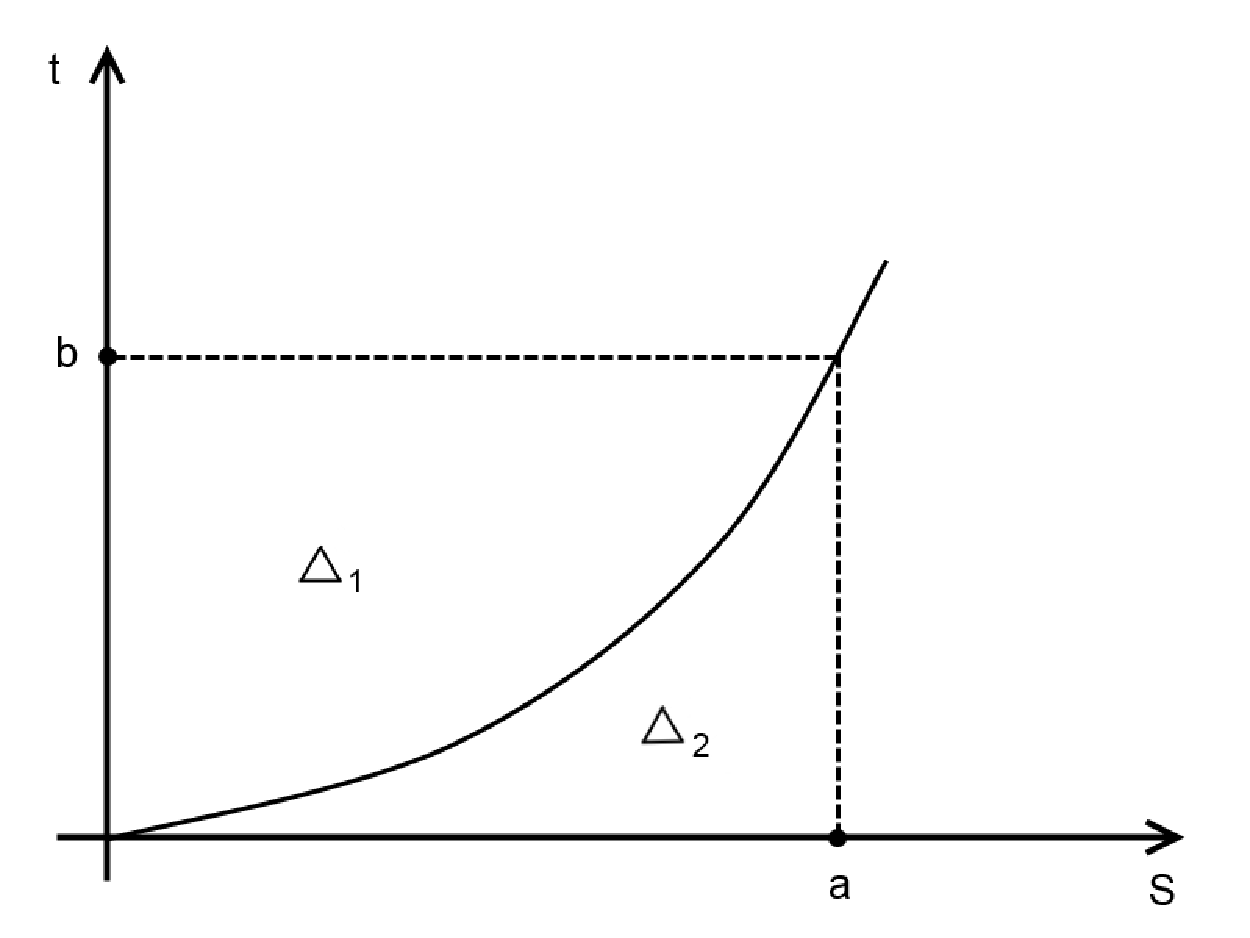
\includegraphics[width=\linewidth]{5}
\end{wrapfigure}

$\frac1p+\frac1q=1$ $\Leftrightarrow$ $p+q=pq$ $\Leftrightarrow$ $(p\hm-1)(q-1)=1$

Рассмотрим график $t=s^{p-1}$, он же $s=t^{q-1}$

рассотрим два криволинейных треугольника

$\triangle_1$ ограничен 0s, графиком и $s=a$

$S(\triangle_1)=\displaystyle\int\limits_0^a s^{p-1}ds=\frac{a^p}{p}$

$S(\triangle_2)=\displaystyle\int\limits_0^b t^{q-1}dt=\frac{b^q}{q}$

Но либо $a^{p-1}>b$, либо $a^{p-1}<b$, либо $a^{p-1}=b$

\begin{figure}[h]
\begin{minipage}[h]{0.3\linewidth}
\center{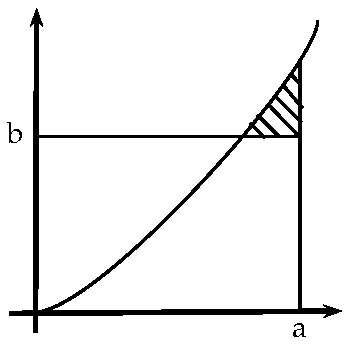
\includegraphics[width=1.0\linewidth]{6} \\ 1.}
\end{minipage}
\hfill
\begin{minipage}[h]{0.3\linewidth}
\center{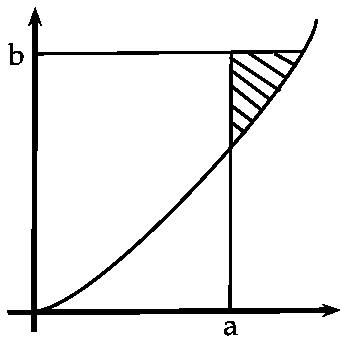
\includegraphics[width=1.0\linewidth]{7} \\ 2.}
\end{minipage}
\hfill
\begin{minipage}[h]{0.3\linewidth}
\center{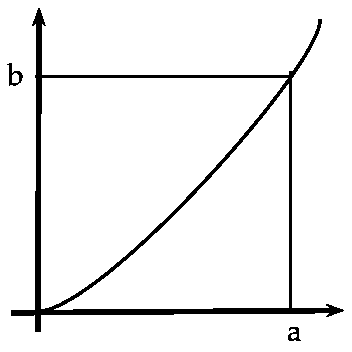
\includegraphics[width=1.0\linewidth]{8} \\ 3.}
\end{minipage}
\end{figure}

В общих случаях 1,2 $ab\le S(\triangle_1)+S(\triangle_2)$. В случае 3 $ab=S(\triangle_1)+S(\triangle_2)$

Неравенство Юнга доказано

Если $\|f\|_p=0$, то $f(x)=0$ почти всюду, $f(x)\cdot g(x)=0$ почти всюду, неравенство превращается в равенство $0=0$

Аналогично при $\|g\|_q=0$

Если $\|f\|_p>0$, $\|g\|_p>0$, то рассмотрим функции 

$\varphi(x)=\displaystyle\frac{f(x)}{\|f\|_p}$, $\psi(x)=\displaystyle\frac{g(x)}{\|g\|_q}$

По неравенству Юнга $\forall x\quad|\varphi(x)\psi(x)|=\displaystyle\frac{|f(x)g(x)|}{\|f\|_p\cdot\|g\|_q}\le\displaystyle\frac{|f(x)|^p}{p\|f\|_p^p}+\displaystyle\frac{|g(x)|^q}{q\|g\|_q^q}$

Проинтегрируем это неравенство:

$\displaystyle\frac1{\|f\|_p\cdot\|g\|_q}\displaystyle\int\limits_X|f(x)g(x)|d\mu\le\frac1{p\|f\|_p^p}\displaystyle\int\limits_X|f(x)|^pd\mu+\frac1{q\|g\|_q^q}\displaystyle\int\limits_X|g(x)|^qd\mu=\frac1p\hm+\frac1q=1$

Домножая на $\|f\|_p\cdot\|g\|_q$, получаем неравенство Гельдера $\blacksquare$
\bigskip

\noindent\textbf{Теорема 11.2:} (Неравенство Минковского) Пусть $(X,M,\mu)$ - пространство с мерой, $f,g$ - измеримые, $p\ge1$, $|f|^p\in L(X)$, $|g|^p\in L(X)$. 
Тогда $|f+g|^p\in L(X)$ и $\|f+g\|_p\le\|f\|_p+\|g\|_p$

\noindent $\square$ Если $p=1$, то утверждение следует из свойств интеграла Лебега, т. к. $|f(x)+g(x)|\le|f(x)|+|g(x)|$

Пусть $p>1$. Заметим, что $|f(x)+g(x)|\le\left(2\max(|f(x)|,|g(x)|)\right)^p\le$

$\noindent\le2^p(|f(x)|^p+|g(x)|^p)$ $\Rightarrow$ $|f+g|^p\in L(X)$

Пусть $q=\frac{p}{p-1}$, тогда $\frac1p+\frac1q=1$

Заметим, что $|f(x)+g(x)|^p=|f(x)+g(x)|^{p-1}\cdot|f(x)+g(x)|\le|f(x)|\hm\cdot|f(x)+g(x)|^{p-1}+|g(x)|\cdot|f(x)+g(x)|^{p-1}$, где $|f(x)+g(x)|^{p-1}=h(x)$

Но $|h(x)|^q=|f(x)+g(x)|^p$ $\Rightarrow$ пары $(f,h)$ и $(g,h)$ удовлетворяют условиям неравенства Гельдера

Тогда $\|f+g\|_p^p\le\displaystyle\int\limits_X|f(x)|\cdot|h(x)|d\mu+\displaystyle\int\limits_X|g(x)|\cdot|h(x)|d\mu\le$(по нер. Гельдера)$\|f\|_p\hm\cdot\|h\|_q+\|g\|_p\cdot\|h\|_q=\left(\|f\|_p+\|g\|_p\right)\cdot\|h\|_q$, где $\|h\|_q=\left(\displaystyle\int\limits_X|f(x)+g(x)|^pd\mu\right)^{1-\frac1p}\hm=\|f+g\|_p^{p-1}$

Если $\|f+g\|_p=0$, то неравенство верно

Иначе сокращаем на $\|f+g\|_p^{p-1}$ и получаем: $\|f+g\|_p\le\|f\|_p+\|g\|_p$ $\blacksquare$
\bigskip

\noindent\textbf{Определение:} Пусть $(X,M,\mu)$ - пространство с мерой, $p\ge1$

$\tilde L_p(X,M,\mu)=\{f\text{ - измеримая на }X\colon|f(x)|^p\in L(X,M,\mu)\}$, а $L_p(X,M,\mu)=\tilde L_p(X,M,\mu)/\sim$ (где $f\sim g$, если $f(x)=g(x)$ почти всюду)
\bigskip

\noindent\textbf{Теорема 11.3:} Если $(X,M,\mu)$ - пространство с мерой, $p\ge1$, то 

$\left(L_p(X,M,\mu),\|f\|_p=\biggl(\displaystyle\int\limits_X|f(x)|^pd\mu\biggr)^\frac1p\right)$ - нормированное пространство

\noindent $\square$ Если $f,g\in\tilde L_p$, то по неравенству Минковского $\|f\|_p\le\|g\|_p+\|f-g\|_p$, $\|g\|_p\le\|f\|_p+\|f-g\|_p$, т. е. $\left|\|f\|_p-\|g\|_p
\right|\le\|f-g\|_p$

$\Rightarrow$ Если $f\sim g$, то $\|f\|_p=\|g\|_p$

То, что $\tilde L_p$ - линейное пространство, следует из неравенства Минковского

Проверим аксиомы нормы:

(3) = неравенство Минковского

(2) $\|\alpha f\|_p=\left(\displaystyle\int\limits_X|\alpha f(x)|^pd\mu\right)^\frac1p=\left(|\alpha|^p\displaystyle\int\limits_X|f(x)|^pd\mu\right)^\frac1p=|\alpha|
\cdot\|f\|_p$

(1) Если $f\in\tilde L_p$, $\|f\|_p=0$, то $f=0$ почти всюду, т. е. $f\sim0$, т. е. $f=0$ в смысле $L_p$

Обратно, если $f=0$ почти всюду, то $\|f\|_p=0$ $\blacksquare$
\bigskip

\noindent\textbf{Лемма 11.1:} Пусть $\mu X<\infty$, $p>1$. Тогда $L_p(X)\in L_1(X)$ и $\exists c=c(p,X)\colon$

\noindent$\forall f\in L_p\quad\|f\|_1\le c\cdot\|f\|_p$ (в частности, если $\|f_n-f\|_p\to0$, то $\|f_n-f\|_1\to0$)

\noindent $\square$ Применим неравенство Гельдера с $g(x)\equiv1$, $q=\frac{p}{p-1}$

Тогда $\|f\|_1=\displaystyle\int\limits_X|f(x)|\cdot 1d\mu\le\|f\|_p\cdot\|1\|_q=(\mu X)^\frac{p-1}{p}\|f\|_p$ $\blacksquare$
\bigskip

\noindent\textbf{Лемма 11.2:} Пусть $\{f_n\}$ - последовательность, фундаментальная в $L_1(X,M,\mu)$. Тогда $\exists \{n_k\}$, $\exists f$ - измеримая : $f_{n_k}(x)\to f(x)$ почти всюду

\noindent $\square$ В силу фундаментальности можно по индукции выбрать такие $\{n_k\}$, $n_{k+1}>n_k\colon\forall n>n_k$ выполнено $\|f_n-f_{n_k}\|<\frac1{2^k}$

Рассмотрим ряд $|f_{n_1}(x)|+\sum\limits_{k=1}^\infty|f_{n_{k+1}}(x)-f_{n_k}(x)|$ и его частичные суммы

$S_N(x)=|f_{n_1}(x)|+\sum\limits_{k=1}^N|f_{n_{k+1}}(x)-f_{n_k}(x)|$

Тогда $S_{N+1}(x)\ge S_N(x)\quad\forall x$ и $\displaystyle\int\limits_X S_N(x)d\mu=\displaystyle\int\limits_X|f_{n_1}(x)|d\mu+\sum\limits_{k=1}^N\displaystyle\int\limits_X|f_{n_{k+1}}(x)\hm-f_{n_k}(x)|d\mu=\|f_{n_1}\|_1+\sum\limits_{k=1}^N\|f_{n_{k+1}}-f_{n_k}\|_1\le\|f_{n_1}\|_1+\sum\limits_{k=1}^N\frac1{2^k}<\|f_{n_1}\|+1$

По теореме Б. Леви $\lim\limits_{N\to\infty}S_N(x)$ конечен почти всюду, т. е. ряд $|f_{n_1}(x)|\hm+\sum\limits_{k=1}^N|f_{n_{k+1}}(x)-f_{n_k}(x)|$ сходится почти всюду

Тем более сходится ряд $f_{n_1}(x)+\sum\limits_{k=1}^\infty\left(f_{n_{k+1}}(x)-f_{n_k}(x)\right)$, но $\sigma_N(x)=f_{n_1}(x)\hm+\sum\limits_{k=1}^N\left(f_{n_{k+1}}(x)-f_{n_k}(x)\right)=f_{n_{N+1}}(x)$

Обозначим $f(x)=\lim\limits_{k\to\infty}f_{n_k}(x)$ там, где $\{\sigma_N(x)\}$ сходится, и доопределим $f\equiv0$ там, где $\{\sigma_N(x)\}$ не сходится 
$\blacksquare$
\bigskip

\noindent\textbf{Лемма 11.3:} Пусть $p>1$, $\{f_n\}$ - фундаментальна в $L_p(X,M,\mu)$. Тогда $\exists\{n_k\}$, $\exists f$ - измеримая : $f_{n_k}\to f$ почти всюду

\noindent $\square$ Если $\mu X<\infty$, то $\{f_{n_k}\}$ - фундаментальная в $L_p$, то по л. 11.1 $\{f_{n_k}\}$ - фундаментальная в $L_1$

($\|f_{n_k}-f_{n_j}\|_p\le c\cdot\|f_{n_k}-f_{n_j}\|_1\le c_\varepsilon$)

Пусть мера $\sigma$ - конечна, т. е. $\exists X_l\in M\colon\mu X_l<\infty$, $X=\bigsqcup\limits_{l=1}^\infty X_l$. По доказанному $\exists\{n_k^{(1)}\}$, $\exists f^{(1)}$  - измеримая на $X_1\colon f_{n_k}^{(1)}\to f^{(1)}$ почти всюду на $X_1$

Из $\{n_k^{(1)}\}$ выберем $\{n_k^{(2)}\}$, которые таковы, что $f_{n_k}^{(2)}$ сходятся почти всюду на $X_2$ к некоторой измеримой $f^{(2)}$

По индуции из $\{n_{k_l}^{(l)}$: $f_{n_k}^{(l)}$ сходится почти всюду на $\bigsqcup\limits_{j=1}^l X_j$, выберем $\{n_k^{(l+1)}\}$: $f_{n_k}^{(l+1)}$ сходится почти всюду на $X_{l+1}$

Рассмотрим подпоследовательность $n_k^{(k)}$. Тогда $\forall\{n_k^{(k)}\}_{k=1}^\infty$ - подпоследовательность в $\{n_j^{(l)}\}_{j=1}^\infty$ $\Rightarrow$ $\{f_{n_k}^{(k)}\}$ сходится почти всюду на $X_l$ $\Rightarrow$ $\{f_{n_k}^{(k)}\}$ сходится всюду на $X$, кроме счетного объединения множеств меры нуль, к $f(x)=\begin{cases}f^{(l)},&\text{если }x\in X_l\text{ - точка сходимости}\\0,&\text{иначе}\end{cases}$ $\blacksquare$
\bigskip

\noindent\textbf{Теорема 11.4:} Пусть $(X,M,\mu)$ - пространство с мерой, $p\ge1$. Тогда нормированное пространство $L_p(X,M,\mu)$ полно

\noindent $\square$ Пусть $\{f_1\}$ - фундаментальная. По лемме 11.3 $\exists\{n_k\}$, $\exists f$ - измеримая : $f_{n_k}\to f$ почти всюду

Но $\{f_{n_k}\}$ - фундаментальная по норме $L_p$ $\Rightarrow$ $\forall\varepsilon>0\quad\exists N\quad\forall k,l>N\quad\|f_{n_k}\hm-f_{n_l}\|_p<\varepsilon$

Функции $\varphi_l(x)=|f_{n_k}(x)-f_{n_l}(x)|^p$

Тогда $\varphi_l(x)\ge0$, $\varphi_l(x)\xrightarrow[l\to\infty]{}|f_{n_k}(x)-f(x)|^p$ почти всюду

$\displaystyle\int\limits_X|f_{n_k}(x)-f(x)|^pd\mu\le\varliminf\limits_{l\to\infty}\displaystyle\int\limits_X\varphi_l(x)d\mu\le\varepsilon^p$, т. е. $\|f_{n_k}-f\|\le\varepsilon$ $(\forall k>N)$

Итак, $f_{n_k}-f\in L_p$, тогда по неравенсвту Минковского $\|f(x)\|=\|f_{n_k}(x)\|\hm+\|\left(f(x)-f_{n_k}(x)\right)\|\in L_p$ и $\forall k>N\quad\|f_{n_k}-f\|_p\le\varepsilon$, т. е. $f_{n_k}\to f$ в норме $L_p$

По лемме 1.2 $f_n\to f$ в $L_p$ $\blacksquare$
\bigskip

\noindent\textbf{Определене:} Пусть $(X,M,\mu)$ - пространство с мерой, 

$\tilde L_\infty(X,M,\mu)=\{f$ - измеримые : $\exists g\sim f\colon g$ - ограниченная на $X\}$, $L_\infty(X,M,\mu)=\tilde L_\infty(X,M,\mu)/\sim$, $\|f\|_\infty=\inf\limits_{g\sim f}\sup\limits_{x\in X}|g(x)|\stackrel{(*)}{=}\inf\left\{c\colon\mu\{x\colon|f(x)|>c\}=0\right\}$
\bigskip

\noindent\textbf{Теорема 11.5:} $\left(L_\infty(X,M,\mu),\|f\|_\infty\right)$ есть банахово пространство

\noindent $\square$ (1) проверим равенство (*)

Если $g\sim f$, $\sup\limits_x|g(x)|=c$, то $\mu\{x\colon|f(x)|>c\}\le\mu\{x\colon f(x)\ne g(x)\}=0$

Обратно, если $\mu\{x\colon|f(x)|>c\}=0$, $g(x)=\begin{cases}f(x),&\text{если }|f(x)|\le c\\0,&\text{если }|f(x)|>c\end{cases}$, 

то $g\sim f$ и $\sup|g(x)|\le c$

(2) Проверим аксиомы нормы

1. Если $\|f\|_\infty=0$, то $f\sim0$

2. Если $g\sim f$, $\sup|g|=c$, то $\alpha g\sim\alpha f$, $\sup|\alpha g|=|\alpha|c$

3. Если $|f|\le c_1$ почти всюду, $|g|\le c_2$ почти всюду, то $|f+g|\le c_1+c_2$ почти всюду

$\Rightarrow$ $\|f+g\|_\infty\le c_1+c_2\colon\inf$ по $c_1$ и $c_2$ дает неравенство треугольника

(3) Проверим полноту

Пусть $\{f_n\}_{n=1}^\infty$ - фундаментальная в $L_\infty$

Пусть $E_n=\{x\colon|f_n(x)|>\|f_n\|_\infty\}$, $E_{n,m}=\{x\colon|f_n(x)-f_m(x)|>\|f_n\hm-f_m\|_\infty\}$

Тогда $\mu E_n=0$, $\mu E_{n,m}=0$

На множестве $X\setminus\underbrace{\left(\bigsqcup\limits_n E_n\sqcup\bigsqcup\limits_{n,m}E_{n,m}\right)}_{\text{меры нуль}}$ $\{f_n\}$ удовлетворяют критерию Коши равномерной сходимости

$\Rightarrow$ $\exists f\colon f_n\rightrightarrows f$ на $X_0$, тогда $\exists N\colon \sup\limits_{X_0}|f_N(x)-f(x)|<1$

Тогда $\sup\limits_{X_0}|f(x)|\le\sup\limits_{X_0}|f_N(x)|+1\le\|f_N\|_\infty+1$

Т. е. $f\in\tilde L_p(X,M,\mu)$ и $\|f_n-f\|_\infty\xrightarrow[n\to\infty]{}0$, т. к. сходимость равномерна на $X_0$ $\blacksquare$







\chapter{Абсолютно непрерывные функции} 

\noindent\textbf{Определение:} Функция $f(x)$ назвается абсолютно непрерывной на $[a,b]$, ($f\in AC([a,b])$), если $\forall\varepsilon>0\quad\exists\delta>0\colon\forall$ системы попарно непересекающихся интервалов $\left\{(a_k,b_k)\right\}_{k=1}^n$ из $[a,b]\subset\sum\limits_{k=1}^n(b_k-a_k)<\delta$ выполнено условие
$\sum\limits_{k=1}^n|f(b_k)-f(a_k)|<\varepsilon$
\bigskip

\noindent\textbf{Лемма 12.1:} Если $\mu$ - классическая мера на $[a,b]$, $f\in C([a,b])$, $F(x)\hm=\displaystyle\int\limits_{[a,x]}f(t)d\mu(t)$, то $F\in AC([a,b])$

\noindent $\square$ Заметим, что $F(b_k)-F(a_k)=\displaystyle\int\limits_{(a_k,b_k]}f(x)d\mu$

$\sum\limits_{k=1}^n|F(b_k)-F(a_k)|\le\sum\limits_{k=1}^n\displaystyle\int\limits_{(a_k,b_k]}|f(x)|d\mu=\displaystyle\int\limits_{\bigsqcup\limits_{k=1}^n(a_k,b_k]}|f(x)|d\mu$, где $\mu\left(\bigsqcup\limits_{k=1}^n(a_k,b_k]\right)\hm=\sum\limits_{k=1}^n(b_k-a_k)$ 

$\Rightarrow$ из т. об абсолютной непрерывности интеграла Лебега получаем утверждение леммы $\blacksquare$
\bigskip

\noindent\textbf{Теорема 12.1:} Если $\mu$ - классическая мера Лебега на $[a,b]$, $f\in AC([a,b])$, то: (1) $f'(x)$ существует почти всюду на $[a,b]$ и $f'\in L([a,b])$

(2) $\forall x\in (a,b]\quad f(x)=f(a)+\displaystyle\int\limits_{[a,x]}f'(t)d\mu(t)$
\bigskip

\noindent\textbf{Лемма 12.2:} Пусть $f,g\in AC(([a,b])$. Тогда $f(x)\cdot g(x)\in AC([a,b])$

\noindent $\square$ Пусть $a\le\alpha\le\beta\le b$. Тогда $fg(\beta)-fg(\alpha)=f(\beta)g(\beta)-f(\beta)g(\alpha)\hm+f(\beta)g(\alpha)-f(\alpha)g(\alpha)-f(\beta)\left(g(\beta)-g(\alpha)\right)+g(\alpha)\left(f(\beta)-f(\alpha)\right)$

Т. к. $f$ и $g$ непрерывны, то $\max\limits_{[a,b]}|f|<\infty$, $\max\limits_{[a,b]}|g|<\infty$

Пусть $\varepsilon>0$. $\exists\delta\colon\forall\{(a_k,b_k)\}$ - попарно непересекающихся из $[a,b]$ выполнено:
$\sum\limits_k|f(b_k)-f(a_k)|<\frac{\varepsilon}{2\max|g|}$, $\sum\limits_k|g(b_k)-g(a_k)|<\frac{\varepsilon}{2\max|f|}$

Тогда $\sum\limits_k|f(b_k)g(b_k)-f(a_k)g(a_k)|\le\max|f|\cdot\sum\limits_k|g(b_k)-g(a_k)|+\max|g|\hm\cdot\sum\limits_k|f(b_k)-f(a_k)|<\varepsilon$ $\blacksquare$
\bigskip

\noindent\textbf{Теорема 12.2:} (Интегрирование по частям) Пусть $\mu$ - классическая мера Лебега на $[a,b]$, $f,g\in AC([a,b])$. Тогда $\displaystyle\int\limits_{[a,b]}f(x)g'(x)d\mu=f(b)g(b)-f(a)g(a)\hm-\displaystyle\int\limits_{[a,b]}f'(x)g(x)d\mu$

\noindent $\square$ $f$ - непрерывная, $g\in L([a,b])$  по т. 12.1(1) $\Rightarrow$ $|f(x)g'(x)|\le\max|f|\cdot|g'(x)|$ и $fg'$ измерима как произведение двух измеримых $\Rightarrow$ $fg'\in L([a,b])$

Аналогично $f'g\in L([a,b])$

По лемме 12.2 $fg\in AC([a,b])$ $\Rightarrow$ по теореме 12.1(2) $f(b)g(b)-f(a)g(a)\hm=\displaystyle\int\limits_{[a,b]}(fg)'(x)d\mu$

\noindent Но $(fg)'(x)=f(x)g'(x)+f'(x)g(x)$ в каждой точке, где $fg'(x)$ и $f'(x)$, т. е. почти всюду

Интегрируя это равенство, получаем утверждение теоремы $\blacksquare$
\bigskip

\noindent\textbf{Лемма 12.3:} Пусть $f$ - строго возрастающая функция из $AC([a,b])$, 

\noindent $f\colon[a,b]\to[c,d]$, и задано $E\subset[c,d]$, $E$ - измеримое относительно классической меры Лебега. Тогда $\mu E=\displaystyle\int\limits_{[c,d]}\chi_E(x)d\mu=\displaystyle\int\limits_{[a,b]}\chi_E\left(f(t)\right)f'(t)d\mu(t)$ $(*)$

\noindent $\square$ (1) Если $E=(\gamma,\delta)$, $f(\alpha)=\gamma$, $f(\beta)=\delta$, то $\displaystyle\int\limits_{[a,b]}\chi_E(f(t))f'(t)d\mu(t)\hm=\displaystyle\int\limits_{[\alpha,\beta]}f'(t)d\mu(t)\stackrel{\text{т. }12.1}{=}f(\beta)-f(\alpha)=\delta-\gamma=\mu E$
\bigskip

(2) Если $E$ - конечное дизъюнктное объединение промежутков $(E\hm\in R(S))$, то $(*)$ получается по линейности

(3) Если $E=\bigsqcup\limits_{n=1}^\infty I_n$, $I_n$ - промежуток, то положим $E_k=\bigsqcup\limits_{n=1}^k I_n$

Тогда $\mu E_k=\displaystyle\int\limits_{[a,b]}\chi_{E_k}(f(t))f'(t)d\mu(t)$, $\chi_{E_k}(f(t))f'(t)\uparrow\chi_E(f(t))f'(t)$ почти всюду и $E=\bigcup\limits_{k=1}^\infty E_k$, $E_k\subset E_{k+1}$

\noindent Переходя к пределу (слева - по теореме о непрерывности меры, справа - по теореме Б. Леви) получаем (*) для множества $E$

(4) Пусть $E=\bigcap\limits_{n=1}^\infty E_n$, где для $E_n$ (*) доказано, и $E_n\supset E_{n+1}$

Тогда $\chi_{E_k}(f(t))f'(t)\le f'(t)\in L$

$f'(t)-\chi_{E_k}(f(t))f'(t)\uparrow f'(t)-\chi_E(f(t))f'(t)$ 

$\Rightarrow$ по т. Леви $\displaystyle\int\limits_{[a,b]}\chi_{E_k}(f(t))f'(t)d\mu(t)\to\displaystyle\int\limits_{[a,b]}\chi_E(f(t))f'(t)d\mu(t)$

$\mu E_k\to\mu E$ в силу конечности меры $\Leftrightarrow$ ее непрерывности сверху

Поэтому (*) верно для $E$
\bigskip

(5) Пусть $E\in\mathfrak M$. Докажем, что $\exists G_n$ - счетное объединение элементов $S$ (промежутков) таких, что $G_n\supset G_{n+1}$, $E=\bigcap\limits_{n=1}^\infty G_n\setminus P$, где $\mu P=0$

Действительно, по определению внешней меры $\exists H_n=\bigcup\limits_{k=1}^\infty I_{n,k}$, $I_{n,k}\hm\in S\colon H_n\supset E$, $\mu(H_n\setminus E)=\mu H_n-\mu_E=\frac1n$

Положим $G_n=\bigcap\limits_{l=1}^n H_l$, тогда $G_n\supset G_{n+1}$, $H_n\supset G_n\supset E$, $\mu(G_n\setminus E)\le$

\noindent$\le\mu(H_n\setminus E)<\frac1n$

По свойству непрерывности меры $\mu\left(\bigcap\limits_{n=1}^\infty(G_n\setminus E)\right)=\mu\left((\bigcap\limits_{n=1}^\infty G_n)\setminus E\right)\hm=\lim\limits_{n\to\infty}\mu(G_n\setminus E)=0$

Но если $H=\bigcup\limits_{n=1}^\infty I_n$, $\tilde H=\bigcup\limits_{k=1}^\infty \EuScript I_k$, где $I_n,\EuScript I_k\in S$, то $H\cap\tilde H=\left(\bigcup\limits_{n=1}^\infty I_n\right)\hm\cap\left(\bigcup\limits_{k=1}^\infty\EuScript I_k\right)=\bigcup\limits_{n,k}(I_n\cap\EuScript I_k)$, где $I_n\cap\EuScript I_k\in S$

По индукции получаем, что $\forall n\quad G_n=\bigcap\limits_{l=1}^n H_l$ есть счетное объединение элементов $S$ (промежутков)

(6) Если $E=\bigcup\limits_{n=1}^\infty I_n$, то $E\bigsqcup\limits_{n=1}^\infty I_n\setminus\left(\bigcup\limits_{k=1}^{n-1}(I_k\cap I_n)\right)$, где $\EuScript I_n=\bigcup\limits_{k=1}^{n-1}(I_k\cap I_n)\hm\in R(S)$ $\Rightarrow$ $\EuScript I_n=\bigsqcup\limits_i\EuScript I_{n,i}$, $\quad\EuScript I_{n,i}\in S$

\noindent $\Rightarrow$ по лемме 3.2 $I_n\setminus\EuScript I_n$ есть конечное дизъюнктное объединение \mbox{элементов $S$}

Тогда $E$ есть счетное дизъюнктное объединение элементов $S$
\smallskip

(7) Пусть $E\in\mathfrak M$, в силу п. 5 $E=\bigcap\limits_{n=1}^\infty G_n\setminus P$, $\mu P=0$, где в силу п. 6 $G_n$ удовлетворяет условиям п. 3 $\Rightarrow$ 
(*) верно для $G_n$

$\Rightarrow$ в силу п. 4 (*) верно для $\bigcap\limits_{n=1}^\infty G_n$, и осталось доказать, что (*) верно для $P$

В силу п. 5 $P=\bigcap\limits_{n=1}^\infty\tilde G_n\setminus\tilde P$, где для $P_1=\bigcap\limits_{n=1}^\infty\tilde G_n$ равенство (*) верно,и $\mu P_1=\mu P+\mu 
\tilde P=0$, т. е. (*) для $P_1$ принимает вид:

$0=\mu P_1=\displaystyle\int\limits_{[a,b]}\chi_{P_1}(f(t))f'(t)d\mu(t)$

Но $P\subset P_1$, $f'(t)\ge0$, то $0\le\chi_P(f(t))f'(t)\le\chi_{P_1}(f(t))f'(t)$

\noindent $\Rightarrow$ $0=\mu P=\displaystyle\int\limits_{[a,b]}\chi_P(f(t))f'(t)d\mu(t)=0$, т. е. (*) верно для $P$ $\Rightarrow$ и для $E$ $\blacksquare$
\bigskip

\noindent\textbf{Теорема 12.3:} Пусть $g\in AC([a,b])$, $g\colon[a,b]\to[c,d]$, $f\in L([a,b])$, $g$ - строго возрастает, $\mu$ - классическая мера Лебега

Тогда $\displaystyle\int\limits_{[c,d]}f(x)d\mu(x)=\displaystyle\int\limits_{[a,b]}f(g(t))g'(t)d\mu(t)$ (**)

\noindent $\square$ Если $f(x)=\chi_E(x)$, $E\in\mathfrak M$, то утверждение доказано в лемме 12.3

По линейности утверждение верно для простых функций. Если $f$ - интегрируемая, неотрицательная, то по л. 7.1 $\exists$ простые неотрицательные $h_n\uparrow f$ и по т. 7.2 $\displaystyle\int\limits_{[c,d]}h_n(x)d\mu(x)\to\displaystyle\int\limits_{[c,d]}f(x)d\mu(x)$

Но $h_n(g(t))g'(t)\uparrow f(g(t))g'(t)$

По теореме Б. Леви $\displaystyle\int\limits_{[a,b]}h_n(g(t))g'(t)d\mu\to\displaystyle\int\limits_{[a,b]}f(g(t))g'(t)d\mu(t)$

$\displaystyle\int\limits_{[a,b]}h_n(g(t))g'(t)d\mu=\displaystyle\int\limits_{[c,d]}h_n(x)d\mu(x)\to\displaystyle\int\limits_{[c,d]}f(x)d\mu(x)<\infty$

Причем $f(g(t))g'(t)\in L([a,b])$ по т. Леви, и (**) верно для $f$

Если $f\in L([a,b])$ - любого знака, то $f=f_+-f_-$ 

$\Bigl(f(g(t))g'(t)=f_+(g(t))g'(t)$, т. к. $g'(t)\ge0\Bigr)$

Поэтому, записывая (*) для $f_+$ и $f_-$ и вычитая, получаем (**) для $f$ $\blacksquare$






\chapter{Преобразование Фурье в $L_1(\mathbb R)$}

\noindent\textbf{Определение:} Пусть $\mu$ - классическая мера Лебега на прямой, $f\in L_1(\mathbb R,\mathfrak M,\mu)$. Ее преобразованием Фурье называется функция $\hat f(\xi)=\displaystyle\frac1{\sqrt{2\pi}}\displaystyle\int\limits_{\mathbb R}f(x)e^{-ix\xi}d\mu(x)$
\bigskip

\noindent\textbf{Замечание:} (1) Определение может отличаться множителем перед интегралом и/или знаком в показателе

(2) (Пока) мы рассматриваем $\xi\in\mathbb R$, но при дополнительных условиях можно рассматривать и $\xi\in\mathbb C$
\bigskip

\noindent\textbf{Определение:} $C_0(\mathbb R)=\{f$ - непрерывная на $\mathbb R\colon\lim\limits_{x\to\pm\infty}f(x)=0\}$, $\|f\|_{C_0(\mathbb R)}\hm=\max\limits_{x\in\mathbb R}|f(x)|$
\bigskip

Несложно видеть, что $C_0(\mathbb R)$ - нормированное пространство
\bigskip

\noindent\textbf{Теорема 13.1:} Пусть $f\in L_1(\mathbb R)$. Тогда:

(1) $\forall\xi\in\mathbb R\quad\exists\hat f(\xi)$

(2) $\hat f\in C_0(\mathbb R)$ и $\|\hat f\|_{C_0}\le\frac1{\sqrt{2\pi}}\|f\|_1$

\noindent $\square$ (1) Т. к. $|e^{-ix\xi}|=1$ при $x\in\mathbb R$, $\xi\in\mathbb R$, то $f(x)e^{-ix\xi}\in L(\mathbb R)$ и $|\displaystyle\int\limits_{\mathbb R}f(x)e^{-ix\xi}d\mu(x)|\hm\le\displaystyle\int\limits_{\mathbb R}|f(x)|d\mu(x)=\|f\|_1$

Если $f(x)=\chi_{[a,b]}(x)$, то $\hat f(\xi)=\displaystyle\frac{e^{-ib\xi}-e^{-ia\xi}}{-i\sqrt{2\pi}\xi}$, $\xi\ne0$ 

$\hat f(0)=\displaystyle\frac1{\sqrt{2\pi}}\displaystyle\int\limits_{[a,b]}d\mu(x)=\frac{b-a}{\sqrt{2\pi}}$

$\lim\limits_{\xi\to0}\hat f(\xi)=\displaystyle\frac{(1-ib\xi)-(1-ia\xi)-o(\xi)}{-i\sqrt{2\pi}\xi}=\frac{b-a}{\sqrt{2\pi}}=\hat f(0)$ $\Rightarrow$ $\hat f\in C_0(\mathbb R)$

Тогда для $f=\sum\limits_{k=1}^n C_k\chi_{[a_k,b_k]}(x)$ выполнено $\hat f\in C_0(\mathbb R)$

Поскольку (!) $\forall f\in L_1\quad\exists f_n$ - линейные комбинации индикаторов такие, что $\|f_n-f\|_1\to0$, то $\sup\limits_\xi|\hat f_n(\xi)-\hat f(\xi)|\le\frac1{\sqrt{2\pi}}\|f_n-f\|_1\to0$, т. е. $\hat f_n(\xi)\rightrightarrows\hat f(\xi)$

Но равномерный предел непрерывных функций непрерывен, а равномерный предел функций, стремящихся к нулю есть функция, стремящаяся к нулю


Поэтому $\hat f\in C_0(\mathbb R)$ $\blacksquare$
\bigskip

\noindent\textbf{Следствие:} Если $f\in L_1(\mathbb R)$, то $\displaystyle\int\limits_{\mathbb R}f(x)\sin(\lambda x)d\mu(x)\xrightarrow[\lambda\to\pm\infty]{}0$

\noindent $\square$ $\displaystyle\int\limits_{\mathbb R}f(x)\sin(\lambda x)d\mu(x)=\displaystyle\int\limits_{\mathbb R}f(x)\frac{e^{i\lambda x}-e^{-i\lambda x}}{2i}d\mu(x)=$

\noindent $=\displaystyle\frac{\sqrt{2\pi}}{2i}\left(\hat f(-\lambda)-\hat f(\lambda)\right)\xrightarrow[\lambda\to\pm\infty]{}0$ $\blacksquare$
\bigskip

\noindent Формула обращения

$f(x)=\displaystyle\frac1{\sqrt{2\pi}}\displaystyle\int\limits_{\mathbb R}\hat f(\xi)e^{ix\xi}d\xi$
\bigskip

Определим $\sigma_R(f,x)=\displaystyle\frac{1}{\sqrt{2\pi}}\displaystyle\int\limits_{-R}^R\hat f(\xi)e^{ix\xi}d\xi$

\noindent\textbf{Лемма 13.1:} Если $f\in L_1(\mathbb R)$, то $\sigma_R(f,x)=\displaystyle\frac1\pi\displaystyle\int\limits_{\mathbb R}f(x+t)\frac{\sin Rt}{t}dt$

\noindent $\square$ $\sigma_R(f,x)=\displaystyle\frac1{2\pi}\displaystyle\int\limits_{-R}^R\displaystyle\int\limits_{\mathbb R}f(t)e^{-i(x-t)\xi}dtd\xi$

Функция $g(t,\xi)=f(t)e^{i(x-t)\xi}$ интегрируемая по Лебегу на $\mathbb R\times[-R,R]$ по теореме Тонелли $\left(\exists\text{ повторный }\displaystyle\int\limits_{-R}^R\displaystyle\int\limits_{\mathbb R}|g(t,\xi)|dtd\xi\right)$

По теореме Фубини можно переставить интегралы: $\sigma_R(f,x)=\displaystyle\int\limits_{\mathbb R}f(t)\displaystyle\int\limits_{-R}^R e^{i(x-t)\xi}d\xi dt\hm=\frac1{2\pi}\displaystyle\int\limits_{\mathbb R}f(t)\frac{e^{i(x-t)R}-e^{-i(x-t)R}}{i(x-t)}dt=\frac1\pi\displaystyle\int\limits_{\mathbb R}f(t)\frac{\sin R(x-t)}{x-t}dt=(t=x+s)\hm=\frac1\pi\displaystyle\int\limits_{\mathbb R}f(x+s)\frac{\sin Rs}{s}ds$ $\blacksquare$
\bigskip

\noindent\textbf{Теорема 13.2:} (Условие Дини) Пусть $f\in L_1(\mathbb R)$, $x\in\mathbb R$ и $\exists\delta>0\colon$ 

$\left|\displaystyle\frac{f(x+t)-f(x)}{t}\right|\in L([-\delta,\delta])$ (как функция $t$). Тогда $f(x)=\lim\limits_{R\to\infty}\sigma_R(f,x)$

\noindent $\square$ Пусть задано $\varepsilon>0$. Т. к. $\displaystyle\int\limits_{\mathbb R}\frac{\sin Rs}{s}ds=\pi$ (несобственный, римановский, $R>0$) то $\exists c_0>0\colon\forall c>c_0\quad\left|\displaystyle\int\limits_{-c}^c\frac{\sin t}{t}dt-\pi\right|<\displaystyle\frac{\varepsilon}{2(1+|f(x)|)}$

Тогда $\forall R>1\quad\left|\displaystyle\int\limits_{-c}^c\displaystyle\frac{\sin Rt}{t}dt-\pi\right|=\left|\displaystyle\int\limits_{-cR}^{cR}\frac{\sin s}{s}ds-\pi\right|<\displaystyle\frac{\varepsilon}{2(1+|f(x)|)}$

Тогда $\left|f(x)-\displaystyle\frac{f(x)}{\pi}\displaystyle\int\limits_{-c}^c\frac{\sin Rt}{t}dt\right|<\displaystyle\frac\varepsilon2$

Но $\left|\sigma_R(f,x)-\displaystyle\frac{f(x)}{\pi}\displaystyle\int\limits_{-c}^c\frac{\sin Rt}{t}dt\right|=\left|\displaystyle\frac1\pi\displaystyle\int\limits_{-c}^c\frac{f(x+t)-f(x)}{t}\sin Rtdt\right|+\left|\displaystyle\frac1\pi\displaystyle\int\limits_{\{|x|>c\}}\frac{f(x+t)}{t}\sin Rtdt\right|\le$

\noindent$\le\left|\displaystyle\frac1\pi\displaystyle\int\limits_{\mathbb R}\frac{f(x+t)-f(x)}{t}\chi_{[-c,c]}(t)\sin Rtdt\right|+\left|\displaystyle\frac1\pi\displaystyle\int\limits_{\mathbb R}\frac{f(x+t)}{t}\chi_{\{|t|\ge c\}}(t)\sin Rtdt\right|$

$\displaystyle\frac{f(x+t)-f(x)}{t}\chi_{[-c,c]}(t)=g_1(t)$, $\displaystyle\frac{f(x+t)}{t}\chi_{\{|t|\ge c\}}(t)=g_2(t)$

Заметим, что $g_1\in L(\mathbb R)$, $g_2\in L(\mathbb R)$

$|g_1(t)|\le\displaystyle\frac{|f(x+t)|+|f(x)|}{\delta}$ при $|t|\ge\delta$, а при $|t|\le\delta$ $g_1$ интегрируема в силу условий Дини

$|g_2(t)|\le\displaystyle\frac{|f(x+t)|}{c}$ $\forall t$

По следствию из т. 13.1 $\displaystyle\int\limits_{\mathbb R}g_1(t)\sin Rtdt\xrightarrow[R\to\infty]{}0$, $\displaystyle\int\limits_{\mathbb R}g_2(t)\sin Rtdt\xrightarrow[R\to\infty]{}0$

При больших $R\colon\left|\sigma_R(f,x)-\displaystyle\frac{f(x)}{\pi}\displaystyle\int\limits_{-c}^c\frac{\sin Rt}{t}dt\right|<\displaystyle\frac{\varepsilon}{2}$, $\left|\sigma_R(f,x)-f(x)\right|<\varepsilon$ $\blacksquare$
\bigskip

\noindent\textbf{Лемма 13.2:} Пусть $f\in L([a,b])$ с классической мерой $\forall c\in(a,b]\quad F(c)=\displaystyle\int\limits_{[a,c]}f(x)d\mu(x)=0$. Тогда $f(x)=0$ почти всюду

\noindent $\square$ Пусть $E=[\alpha,\beta]\in S$ - полукольцо промежутков

Тогда $\displaystyle\int\limits_E f(x)d\mu=F(\beta)-F(\alpha)=0$

Тогда $\forall B\in R(S)\quad\displaystyle\int\limits_B f(x)d\mu=0$

Пусть $A\in\mathfrak M$. $\forall\varepsilon>0\quad\exists\delta>0\colon$ если $\mu E<\delta$, то $\displaystyle\int\limits_E|f(x)|d\mu<\varepsilon$, но 

\noindent $\exists B\in R(S)\colon\mu(A\triangle B)<\delta$

Тогда $\left|\displaystyle\int\limits_A fd\mu-\displaystyle\int\limits_B fd\mu\right|\le\displaystyle\int\limits_{A\triangle B}|f|d\mu<\varepsilon$

Т. к. $A$ - фиксированное, $\varepsilon$ - любое, то $\displaystyle\int\limits_A fd\mu=0$

Предположим, что $f\nsim0$. Для определенности пусть $\mu\{x\colon f(x)>0\}>0$

Т. к. $\{x\colon f(x)>0\}=\bigcup\limits_{n=1}^\infty\{x\colon f(x)>\frac1n\}$ $\exists n_0\colon\mu A_{n_0}=\mu\{x\colon f(x)>\displaystyle\frac{1}{n_0}>0$

$\displaystyle\int\limits_{A_{n_0}}f(x)d\mu\ge\frac{\mu A_{n_0}}{n_0}>0$

Противоречие, следовательно $f(x)=0$ почти всюду $\blacksquare$
\bigskip

\noindent\textbf{Теорема 13.3:} (единственности) Пусть $f\in L_1(\mathbb R)$ и $\hat f(\xi)=0\quad\forall\xi$. Тогда $f(x)=0$ почти всюду

\noindent $\square$ Положим $F_y(x)=\displaystyle\int\limits_{[0,y]}f(x+t)dt=\displaystyle\int\limits_{[x,x+y]}f(t)dt$

Фиксируем $y$: $\displaystyle\int\limits_{\mathbb R}|F_y(x)|dy=\displaystyle\int\limits_{\mathbb R}\left|\displaystyle\int\limits_{[0,y]}f(x+t)dt\right|dx\le\displaystyle\int\limits_{\mathbb R}\displaystyle\int\limits_{[0,y]}|f(x+t)|dtdx\hm=\displaystyle\int\limits_{[0,y]}\displaystyle\int\limits_{\mathbb R}|f(x+t)|dxdt=y\|f\|_{L_1(\mathbb R)}<\infty$ $\Rightarrow$ $F_y(x)\in L_1(\mathbb R)$

$\hat F_y(\xi)=\displaystyle\frac{1}{\sqrt{2\pi}}\displaystyle\int\limits_{\mathbb R}F_y(x)e^{-ix\xi}dx=\displaystyle\int\limits_{\mathbb R}\displaystyle\int\limits_{[0,y]}f(x+t)dt e^{-ix\xi}dx=\displaystyle\int\limits_{[0,y]}\displaystyle\int\limits_{\mathbb R}f(x+t)e^{-i(x+t)\xi}dx e^{it\xi}dt=$

\noindent =(перестановка по т. Тонелли и т. Фубини)$=\displaystyle\int\limits_{[0,y]}0\cdot e^{it\xi}dt=0$

Т. к. $F_y(x)=\displaystyle\int\limits_{[x,x+y]}f(t)dt$, то $F_y(x)\in AC([a,b])$ на любом $[a,b]\subset \mathbb R$, т. е. $F_y(x)$ дифференцируема почти всюду на каждом отрезке, т. е. почти всюду на $\mathbb R$

Но если $\exists F_y'(x_0)$, то $\displaystyle\int\limits_{-\delta}^\delta\left|\frac{F_y(x_0+t)-F_y(x_0)}{t}\right|dt<\infty$

$\Rightarrow$ в каждой точке дифференцируемости выполнено условие Дини 

$\Rightarrow$ $F_y(x)=0$ почти всюду, но $F_y(x)$ непрерывна $\Rightarrow$ $F_y(x)=0\quad\forall x\forall y$

Фиксируем $x=0\colon\forall y\quad\displaystyle\int\limits_{[0,y]}f(t)dt=0$

По лемме 13.2 $f(t)=0$ почти всюду на $[0,y]$, т. е. почти всюду на $\mathbb R$ $\blacksquare$
\bigskip

\noindent\textbf{Теорема 13.4:} Пусть $f\in AC[a,b]\quad\forall a,b\in\mathbb R$, $f\in L_1(\mathbb R)$, $f'\in L_1(\mathbb R)$. Тогда $\hat f'(\xi)=i\xi\hat f(\xi)$

\noindent $\square$ Т. к. $f\in L_1(\mathbb R)$ и $f$ непрерывна, то $\exists a_n\to-\infty$, $\exists b_n\to+\infty\colon f(a_n)\to0$, $f(b_n)\to0$

На $[a_n,b_n]$ запишем формулу интегрирования по частям: 

$\displaystyle\frac{1}{\sqrt{2\pi}}\displaystyle\int\limits_{a_n}^{b_n}f'(x)e^{-ix\xi}dx=f(x)e^{-ix\xi}\Bigl|_{a_n}^{b_n}-\frac{1}{\sqrt{2\pi}}\displaystyle\int\limits_{a_n}^{b_n}f(x)\cdot(-i\xi)e^{-ix\xi}dx$

В пределе при $n\to\infty$ получаем утверждение теоремы $\blacksquare$
\bigskip

\noindent\textbf{Следствие:} Пусть $n\ge1$, $f\in C^{(n-1)}([a,b])$, $f^{(n-1)}\in AC([a,b])$, 

\noindent $f,f',\ldots,f^{(n)}\in L(\mathbb R)$. 
Тогда: (1) $\widehat{f^{(n)}}(\xi)=(i\xi)^n\hat f(\xi)$

(2) $\hat f(\xi)=o\left(\frac{1}{|\xi|^n}\right)$ при $|\xi|\to\infty$

\noindent $\square$ (1) получается из теоремы по индукции $(\widehat{f^{(n)}}(\xi)=i\xi\widehat{f^{(n-1)}}(\xi)=\ldots)$

(2) В силу п. (1) и теоремы 13.1 $\widehat{f^{(n)}}(\xi)=(i\xi)^n\hat f(\xi)\xrightarrow[|\xi|\to\infty]{}0$ $\blacksquare$
\bigskip

\noindent\textbf{Теорема 13.5:} (1) Пусть $f(x,y)$ определена на $X\times[y_0-\delta,y_0+\delta]$,

 $\forall x\quad f(x,y)\in C^{(1)}([y_0-\delta,y_0+\delta])$ как функция $y$,

 $\forall y\quad f(x,y)\in L(X,\mathfrak M,\mu)$ как функция $x$,

 $\exists y(x)\in L(X,\mathfrak M,\mu)\colon\forall y\in[y_0-\delta,y_0+\delta]\quad\forall x\in X\quad |f_y'(x,y)|\le g(x)$. 

Тогда $\exists\displaystyle\frac{d}{dy}\displaystyle\int\limits_X f(x,y)d\mu(x)=\displaystyle\int\limits_X\frac{\partial}{\partial y}f(x,y)d\mu(x)$

(2) Пусть $f(x,z)$ определена на $X\times\{|z-z_0|<\delta\}$, $z\in\mathbb C$, 

$\forall x\quad f(x,z)$ голоморфна в $\{|z-z_0|<\delta\}$, $\forall z\quad f(x,z)\in L(X,\mathfrak M,\mu)$ как функция $x$, $\exists g\in L(X)\colon\forall z,|z-z_0|<\delta\quad\forall x\in X\quad\left|\displaystyle\frac{\partial}{\partial z}f(x,z)\right|\le g(x)$

Тогда существует  $\mathbb C$-производная $\displaystyle\frac{d}{dz}\displaystyle\int\limits_Xf(x,z)d\mu(x)=\displaystyle\int\limits_X\frac{\partial}{\partial z}f(x,z)d\mu(x)$

\noindent $\square$ Докажем п. 1, п. 2 доказывается аналогично

Пусть $F(y)=\displaystyle\int\limits_Xf(x,y)d\mu(x)$. Рассмотрим последовательность $y_n\to y:$

$\displaystyle\frac{F(y_n)-F(y)}{y_n-y}=\displaystyle\int\limits_X\frac{f(x,y_n)-f(x,y)}{y_n-y}d\mu(x)$, 

где $\displaystyle\frac{f(x,y_n)-f(x,y)}{y_n-y}\xrightarrow[n\to\infty]{}f_y'(x,y)\forall x$

Докажем, что можно осуществить предельный переход

Заметим, что $\left|\displaystyle\frac{f(x,y_n)-f(x,y)}{y_n-y}\right|=\left|\displaystyle\frac{1}{y_n-y}\cdot\displaystyle\int\limits_y^{y_n}f_y'(x,u)du\right|\le$

\noindent $\le\displaystyle\frac{1}{|y_n-y|}\cdot|y-y_n|g(x)\le g(x)\quad\forall n$ 

$\Rightarrow$ применима т. Лебега $\Rightarrow$ $\exists\lim\limits_{n\to\infty}\displaystyle\frac{F(y_n)-F(y)}{y_n-y}=\displaystyle\int\limits_Xf_y'(x,y)d\mu(x)$

Т. к. $\{y_n\}$ - любая, а предел справа от нее не зависит, то 

$\exists F'(y)=\displaystyle\int\limits_Xf_y'(x,y_0)d\mu(x)$ $\blacksquare$
\bigskip

\noindent\textbf{Теорема 13.6:} (1) Пусть $f(x)\in L_1(\mathbb R)$, $xf(x)\in L_1(\mathbb R)$. тогда $\exists\hat f'(\xi)=-i\widehat{xf}(\xi)$

(2) Если $f(x),xf(x),\ldots,x^n f(x)\in L_1(\mathbb R)$, то $\exists\hat f^{(n)}(\xi)=(-i)^n\widehat{x^n f}(\xi)$

(3) Если $\exists a>0\colon f(x)e^{a|x|}\in L_1(\mathbb R)$, то $\hat f(\xi)$ продолжается с $\mathbb R$ до функции, голоморфной в полосе $\{|Im\xi|<a\}$

\noindent $\square$ (1) Получается из п. (1) теоремы 13.5

$\displaystyle\frac{d}{d\xi}\frac{1}{\sqrt{2\pi}}\displaystyle\int\limits_{\mathbb R}f(x)e^{-ix\xi}dx=\frac{1}{\sqrt{2\pi}}\displaystyle\int\limits_{\mathbb R}f(x)(-ix)e^{-ix\xi}dx$, 

т. к. $|f(x)\cdot(-ix)e^{-ix\xi}|\le|xf(x)|$

(2) Получается из (1) по индукции

(3) Получается из п. (2) теоремы 13.5

Если $\xi=\alpha+i\beta$, $|\beta|<a$, то $|f(x)e^{-ix\xi}|=|f(x)e^{-ix(\alpha+i\beta}|=|f(x)e^{x\beta}|\le$

\noindent $\le|f(x)e^{a|x|}|$ $\Rightarrow$ $\displaystyle\frac{1}{\sqrt{2\pi}}\displaystyle\int\limits_{\mathbb R}f(x)e^{-ix\xi}dx$ сходится при $|\beta|<a$, 

$|xf(x)e^{-ix\xi}|\le|xf(x)e^{|x\beta|}|\le c|f(x)|e^{a|x|}$ (т. к. $|x|<e^{\delta|x|}$), где $c=c(\delta)$ 

$\Rightarrow$ применима т. 13.5(2)

$\exists\displaystyle\frac{d}{ds}\displaystyle\int\limits_{\mathbb R}f(x)e^{-ix\xi}dx=\frac{1}{\sqrt{2\pi}}\displaystyle\int\limits_{\mathbb R}xf(x)e^{-ix\xi}dx$ $\blacksquare$






\chapter{Интеграл Римана-Стилтьеса}

\noindent\textbf{Определение:} Пусть $f$ и $\varphi$ - две функции на $[a,b]$, $T=\left(\{x_k\},\{\xi_k\}\right)$ - размеченное разбиение $[a,b]$

Интегральной суммой Римана-Стилтьеса называется 

$S_T(f,d\varphi)=\sum\limits_{k=1}^n f(\xi_k)\left(\varphi(x_k)-\varphi(x_{k-1})\right)$

Если $\exists\lim\limits_{\delta_T\to0}S_T(f,d\varphi)$, то он называется интегралом Римана-Стилтьеса $(R-S)\displaystyle\int\limits_a^b fd\varphi$ $\left(\text{где }\delta_T=\max\limits_k(x_k-x_{k-1})\right)$
\bigskip

\noindent\textbf{Свойства:} (1) Если $\exists\displaystyle\int\limits_a^bf_1d\varphi$ и $\exists\displaystyle\int\limits_a^b f_2d\varphi$, то $\exists \displaystyle\int\limits_a^b(\alpha f_1+\beta f_2)d\varphi=\alpha\displaystyle\int\limits_a^b f_1d\varphi\hm+\beta\displaystyle\int\limits_a^b f_2d\varphi$

(2) Если $\exists\displaystyle\int\limits_a^b fd\varphi_1$ и $\exists\displaystyle\int\limits_a^b fd\varphi_2$, то $\exists \displaystyle\int\limits_a^b fd(\alpha\varphi_1+\beta\varphi_2)=\alpha\displaystyle\int\limits_a^b fd\phi_1+\beta\displaystyle\int\limits_a^b fd\phi_2$
\bigskip

\noindent\textbf{Определение:} Пусть $T$ - разбиение отрезка $[a,b]$, $\varphi$ - функция $[a,b]$. Вариационной суммой называется $V_T(\varphi)=\sum\limits_{k=1}^n\left|\varphi(x_k)-\varphi(x_{k-1})\right|$

Вариацией $\varphi$ на $[a,b]$ называется $V_a^b\varphi=\sup\limits_T V_T(\varphi)$

Класс функций ограниченной вариации $BV([a,b])=\{\varphi\colon V_a^b\varphi<\infty\}$
\bigskip

\noindent\textbf{Свойства:} (1) Если $\varphi$ - монотонная, то $\varphi\in BV([a,b])$

(2) Если $\varphi,\psi\in BV([a,b])$, то $\alpha\varphi+\beta\psi\in BV([a,b])$

(3) Если $\varphi\in BV([a,b])$, то $\varphi$ есть разность двух монотонных функций

(4) $AC([a,b])\subset BV([a,b])$
\bigskip

\noindent\textbf{Теорема 14.1:} Пусть $f\in C([a,b])$, $\varphi\in BV([a,b])$. Тогда $\exists (R-S)\displaystyle\int\limits_a^bfd\varphi$

\noindent $\square$ Пусть $\{T_n\}$ - последовательность размеченных разбиений с $\delta_{T_n}\to0$. $\bar T_n$ и $\bar T_m$ - соответствующие неразмеченные разбиения

Возьмем разбиения $T_n=\{x_k\},\{\xi_k\}$ и $T_m=\{y_j\},\{\eta_j\}$. Пусть $T_{n,m}\hm=\bar T_n\cap\bar T_m=\{z_i\}$

$\forall i\quad\exists j=j(i)\colon[z_{i-1},z_i]\subset[y_{j-1},y_j]$, $\exists k=k(i)\colon[z_{i-1},z_i]\subset[x_{k-1},x_k]$

Тогда $S_{T_n}(f,d\varphi)=\sum\limits_k f(\xi_k)\left(\varphi(x_k)-\varphi(x_{k-1})\right)=\sum\limits_i f(\xi_{k(i)})\left(\varphi(z_i)-\varphi(z_{i-1})\right)$

$S_{T_m}(f,d\varphi)=\sum\limits_j f(\eta_j)\left(\varphi(y_j)-\varphi(y_{j-1})\right)=\sum\limits_i f(\eta_{j(i)})\left(\varphi(z_i)-\varphi(z_{i-1})\right)$

Тогда $|S_{T_n}(f,d\varphi)-S_{T_m}(f,d\varphi)|\le\left|\sum\limits_i(f(\xi_{k(i)})-f(\eta_{j(i)})\right|\cdot|\varphi(z_i)-\varphi(z_{i-1})|\le$

\noindent$\le\sum\limits_i\left|f(\xi_{k(i)}-f(\eta_{j(i)})\right|\cdot\left|\varphi(z_i)-\varphi(z_{i-1})\right|\le\left(\sup\limits_{\substack{t_1,t_2\colon\\|t_1-t_2|<\delta_{T_n}+\delta_{T_m}}}|f(t_1)-f(t_2)|\right)\hm\cdot V_{T_{n,m}}(\varphi)\le\left(\sup\limits_{\substack{t_1,t_2\colon\\|t_1-t_2|<\delta_{T_n}+\delta_{T_m}}}|f(t_1)-f(t_2)|\right)\cdot V_a^b\varphi\xrightarrow[n,m\to\infty]{}0$ по т. Кантора о равномерной непрерывности $\blacksquare$
\bigskip

\noindent\textbf{Теорема 14.2:} Пусть $f\in C([a,b])$, $\varphi\in C^{(1)}([a,b])$

 Тогда $\exists(R-S)\displaystyle\int\limits_a^b fd\varphi=(R)\displaystyle\int\limits_a^b f(x)\varphi'(x)dx$

\noindent $\square$ Пусть $T$ - неразмеченное разбиение $\{x_k\}$

Тогда $\exists\xi_l\in[x_{k-1},x_k]\colon\varphi(x_k)-\varphi(x_{k-1})=\varphi'(\xi_k)(x_k-x_{k-1})$

Положим $T=(\{x_k\},\{\xi+k\})$. Тогда $S_T(f,d\phi)=\sum f(\xi_k)\varphi'(\xi-k)(x_k\hm-x_{k-1})=S_t(f\varphi',dx)\to\displaystyle\int\limits_a^b f\varphi'dx$ при $\delta_T\to0$

Но $\displaystyle\int\limits_a^b fd\varphi$ существуют, т. к. $\varphi\in BV([a,b])$ $\Rightarrow$ $S_T(f,d\varphi)\to\displaystyle\int\limits_a^b fd\varphi$

Действительно, $\forall\bar T$ - неразмеченного разбиения $V_{\bar T}(\varphi)=\sum|\varphi(x_k)\hm-\varphi(x_{k-1})|\le\sum\left|\displaystyle\int\limits_{x_{k-1}}^{x_k}\varphi'(t)dt\right|\le\displaystyle\int\limits_a^b|\varphi'(t)|dt<\infty$ $\blacksquare$
\bigskip

\noindent\textbf{Теорема 14.3:} Пусть $\varphi$ - неубывающая непрерывная слева функция на $[a,b]$, $m_\varphi$ - мера Стилтьеса, $\mu_\varphi$ - мера Лебега-Стилтьеса (ее продолжение по Лебегу), $f$ - ограничена и $\mu_\varphi$ почти всюду непрерывна на $[a,b]$

Тогда $\exists(R-S)\displaystyle\int\limits_a^b fd\varphi=(L)\displaystyle\int\limits_{[a,b]}fd\mu_{\varphi}$

\noindent $\square$ Пусть $\{T_n\}$ - последовательность размеченных разбиений с $\delta_{T_n}\to0$

 Тогда $S_{T_n}(f,d\varphi)=\sum\limits_k(\xi_{n,k})(\varphi(x_{n,k})-\varphi(x_{n,k-1}))=\sum\limits_k f(\xi_{n,k})\mu_\varphi[x_{n,k-1},x_{n,k})\hm=\displaystyle\int\limits_{[a,b]}f_n(x)d\mu_\varphi$, где $f_n(x)=\sum f(\xi_{n,k})\cdot\chi_{[x_{n,k-1},x_{n,k})}(x)$

Но $f(x)-f_n(x)=f(x)-f(\xi_{n,k(x)})$, где $|x-\xi_{n,k(x)}|<\delta_{T_n}$

$\Rightarrow$ $f_n(x)\to f(x)$ в каждой точке непрерывности $f$

$\exists M\colon\forall x\quad|f(x)|\le M$ $\Rightarrow$ $\forall x\forall n\quad|f_n(x)|\le M$

Т. к. $\mu_\varphi[a,b)=\varphi(b)-\varphi(a)<\infty$, то $g(x)\equiv M$ - интегрируемая мажоранта

$\Rightarrow$ по т. Лебега $S_{T_n}(f,d\varphi)=\displaystyle\int\limits_{[a,b)}f_n d\mu_\varphi\to\displaystyle\int\limits_{[a,b)}f d\mu_\varphi$ $\blacksquare$
\bigskip

\noindent\textbf{Утверждение 1:} Если $a<c<b$, то $V_a^b f=V_a^c f+V_c^b f$

\noindent $\square$ Если $T_1$ - разбиение $[a,c]$, $T_2$ - разбиение $[c,b]$, то $T_1\cup T_2$ - разбиение $[a,b]$ и $V_{T_1}(f)+V_{T_2}(f)=V_{T_1\cup T_2}(f)\le V_a^b f$

Слева переходим к $\sup\limits_{T_1}$, а затем к $\sup\limits_{T_2}$. Получаем $V_a^c f+V_c^b\le V_a^b f$

Обратно, если $T$ - разбиение $f$, то положим $T'=T\cup\{c\}$, $T_1=T'\cap[a,c]$ - разбиение $[a,c]$, $T_2=T'\cap[c,b]$ - разбиение $[c,b]$

Тогда $V_t(f)\le V_{T'}(f)=V_{T_1}(f)+V_{T_2}(f)\le V_a^c f+V_c^b f$

Слева переходим к $\sup\limits_T$, получим $V_a^b f\le V_a^c f+V_c^b f$ $\blacksquare$
\bigskip

\noindent\textbf{Утверждение 2:} Всякая функция ограниченной вариации есть разность двух неубывающих 

\noindent $\square$ $f\in BV([a,b])$, $f_1(x)=V_a^x f$, $f_2(x)=V_a^x f-f(x)$

Если $x<y$, то $f_1(y)-f_1(x)=V_a^y f-V_a^x f\stackrel{\text{утв. 1}}{=}V_x^y f\ge0$

\noindent$f_2(y)-f_2(x)=V_x^y f-(f(y)-f(x))$, но $|f(y)-f(x)|\le V_x^y f=f_2(y)-f_2(x)$ $\blacksquare$



\end{document}
